
\subsection{Huấn luyện nhiều mô mạng neural đa lớp}
\subsubsection{Bảng kết quả thực nghiệm - mạng neural cùng độ sâu 1 lớp ẩn}

\begin{table} [H]
    \begin{center}
        \caption{Kết quả thực nghiệm bài 4-bit 1 lớp ẩn}

    \begin{tabular}{|c|c|c|c|}
    \hline
    \multirow{1}{*}{\textbf{Method}} & \multicolumn{1}{c|}{\textbf{Subtask1}} & \multicolumn{1}{c|}{\textbf{Subtask 2}} & \multicolumn{1}{c|}{\textbf{Subtask 3}} \\ \hline
    CEA & $0.0316 \pm 0.0125$ & $0.0201 \pm 0.011922$ & $0.0117 \pm 0.008133$ \\
    MFEA-I & $0.025 \pm 0.012957$ & $0.0117 \pm 0.007342$ & $0.0072 \pm 0.005355$\\
    MFEA-II  & $\mathbf{0.0219 \pm 0.009181}$ & $\mathbf{0.0099 \pm 0.007053}$ & $\mathbf{0.0052 \pm 0.004126}$ \\\hline
    
    \end{tabular}
    \end{center}
    
    \label{tab:result:nbit}
\end{table}
\begin{table} [H]   
    \begin{center}
        \caption{Kết quả thực nghiệm bài 6-bit 1 lớp ẩn}

    \begin{tabular}{|c|c|c|c|}
    \hline
    \multirow{1}{*}{\textbf{Method}} & \multicolumn{1}{c|}{\textbf{Subtask1}} & \multicolumn{1}{c|}{\textbf{Subtask 2}} & \multicolumn{1}{c|}{\textbf{Subtask 3}} \\ \hline
    CEA(5,6,7)  & $0.0703 \pm 0.014543$ & $0.0619 \pm 0.018078$ & $0.0572 \pm 0.017982$ \\
    MFEA-I(5,6,7)   & $\mathbf{0.06 \pm 0.014702}$ & $\mathbf{0.0498 \pm 0.009562}$ & $0.047 \pm 0.008464$ \\
    MFEA-II(5,6,7)  & $0.06 \pm 0.011387$ & $0.052 \pm 0.009393$ & $\mathbf{0.047 \pm 0.009579}$ \\\hline
    
    CEA(6,7,8)   & $0.0669 \pm 0.016032$ & $0.0583 \pm 0.009948$ & $0.0521 \pm 0.015598$ \\
    MFEA-I(6,7,8)  & $0.0611 \pm 0.013622$ & $0.0528 \pm 0.011122$ & $0.0484 \pm 0.011074$ \\
    MFEA-II(6,7,8) & $\mathbf{0.0522 \pm 0.011066}$ & $\mathbf{0.0476 \pm 0.01033}$ & $\mathbf{0.0418 \pm 0.011741}$ \\\hline
    
    \end{tabular}
    \end{center}
    \label{tab:result:nbit}
\end{table}    
\begin{table} [H]
    \begin{center}
        \caption{Kết quả thực nghiệm bài 8-bit 1 lớp ẩn}

    \begin{tabular}{|c|c|c|c|}
    \hline
    \multirow{1}{*}{\textbf{Method}} & \multicolumn{1}{c|}{\textbf{Subtask1}} & \multicolumn{1}{c|}{\textbf{Subtask 2}} & \multicolumn{1}{c|}{\textbf{Subtask 3}} \\ \hline
    CEA(5,6,7) & $0.0956 \pm 0.013764$ & $0.0906 \pm 0.015274$ & $0.0874 \pm 0.010884$ \\
    MFEA-I(5,6,7) & $0.0859 \pm 0.011722$ & $0.0801 \pm 0.009489$ & $0.0778 \pm 0.010507$  \\
    MFEA-II(5,6,7) & $\mathbf{0.0827 \pm 0.010678}$ & $\mathbf{0.076 \pm 0.012979}$ & $\mathbf{0.0735 \pm 0.012598}$ \\\hline
    
    CEA(6,7,8)& $0.0895 \pm 0.012499$ & $0.0902 \pm 0.013171$ & $0.081 \pm 0.013371$ \\
    MFEA-I(6,7,8)  & $0.0826 \pm 0.011089$ & $0.0768 \pm 0.010228$ & $0.0734 \pm 0.008805$ \\
    MFEA-II(6,7,8) & $\mathbf{0.0808 \pm 0.010726}$ & $\mathbf{0.0739 \pm 0.01117}$ & $\mathbf{0.072 \pm 0.009657}$ \\\hline
    \end{tabular}
    \end{center}
    \label{tab:result:nbit}
\end{table}

\subsubsection{Biểu đồ hội tụ - mạng neural cùng độ sâu 1 lớp ẩn}
\begin{figure}[H]
    \centering

    \scalebox{.7}{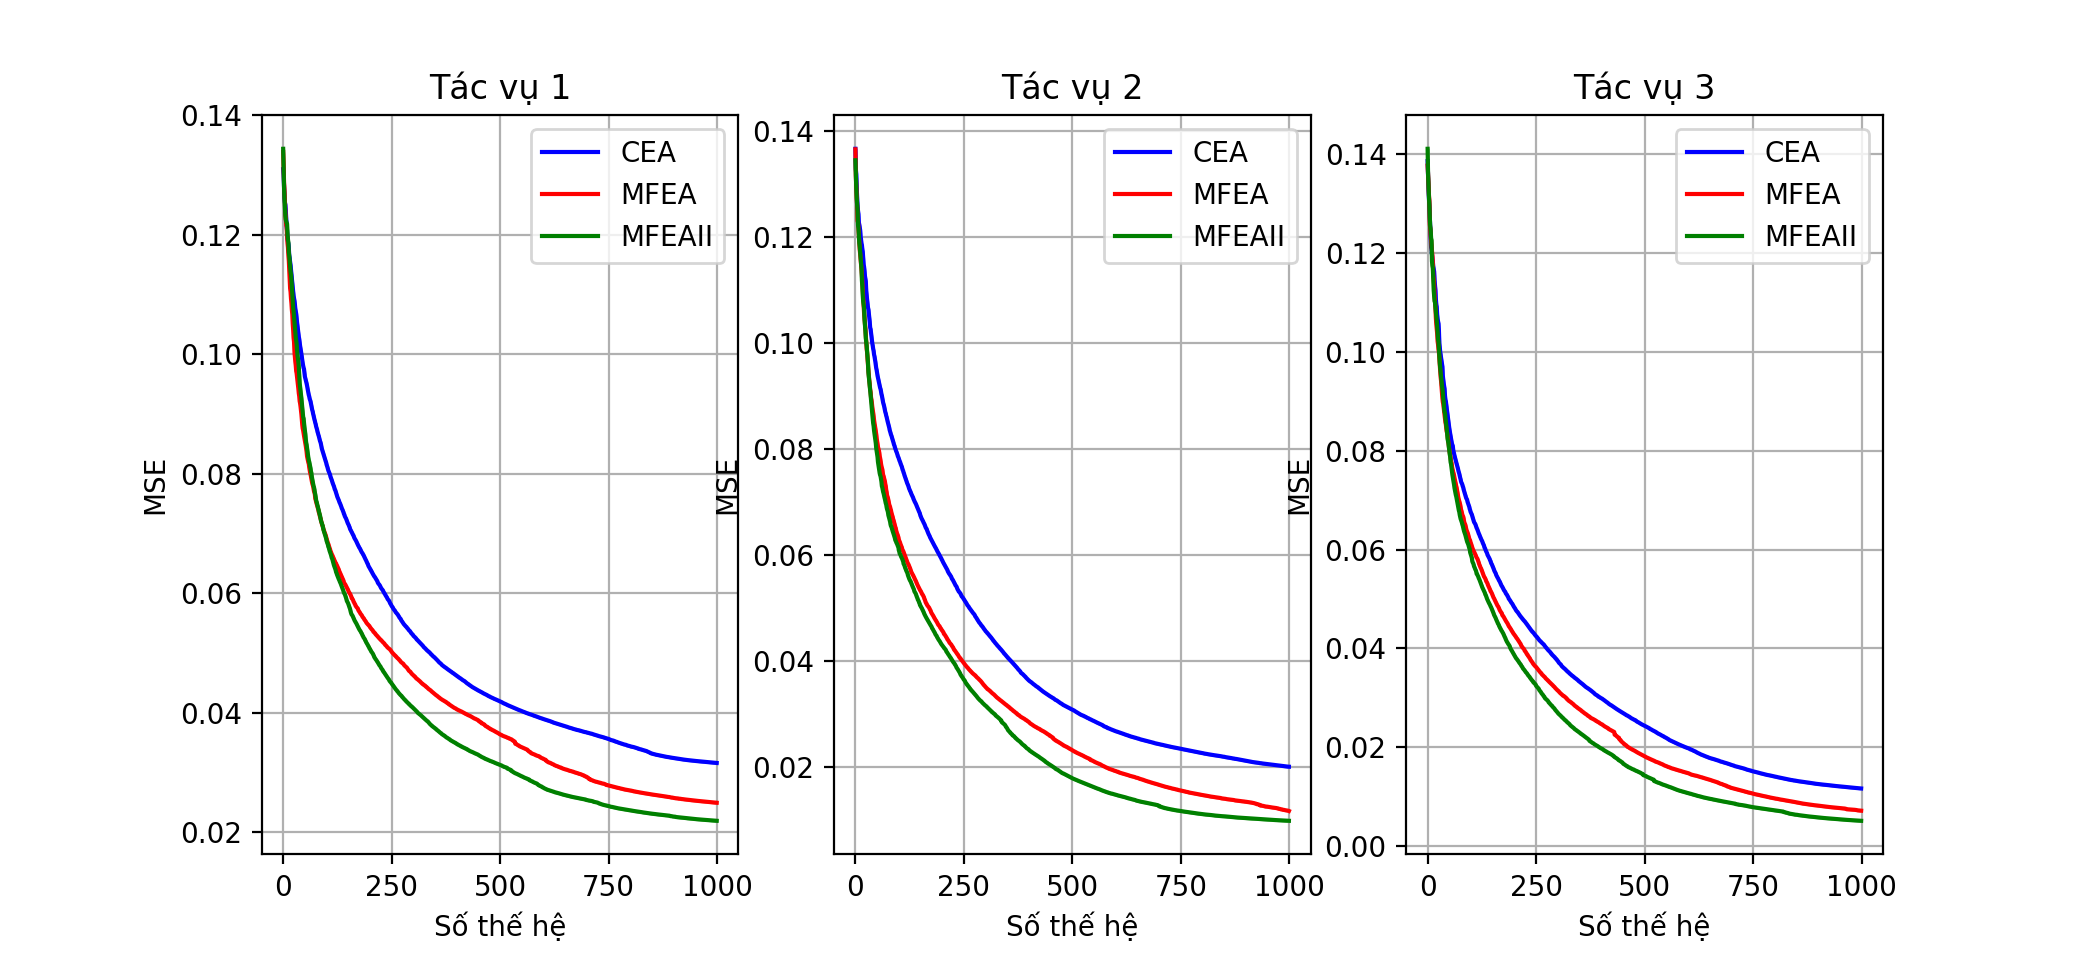
\includegraphics[width=\textwidth,height=\textheight,keepaspectratio]{thesis/images/results/nbit_1layer/4bit_task.png}}
    \scalebox{.7}{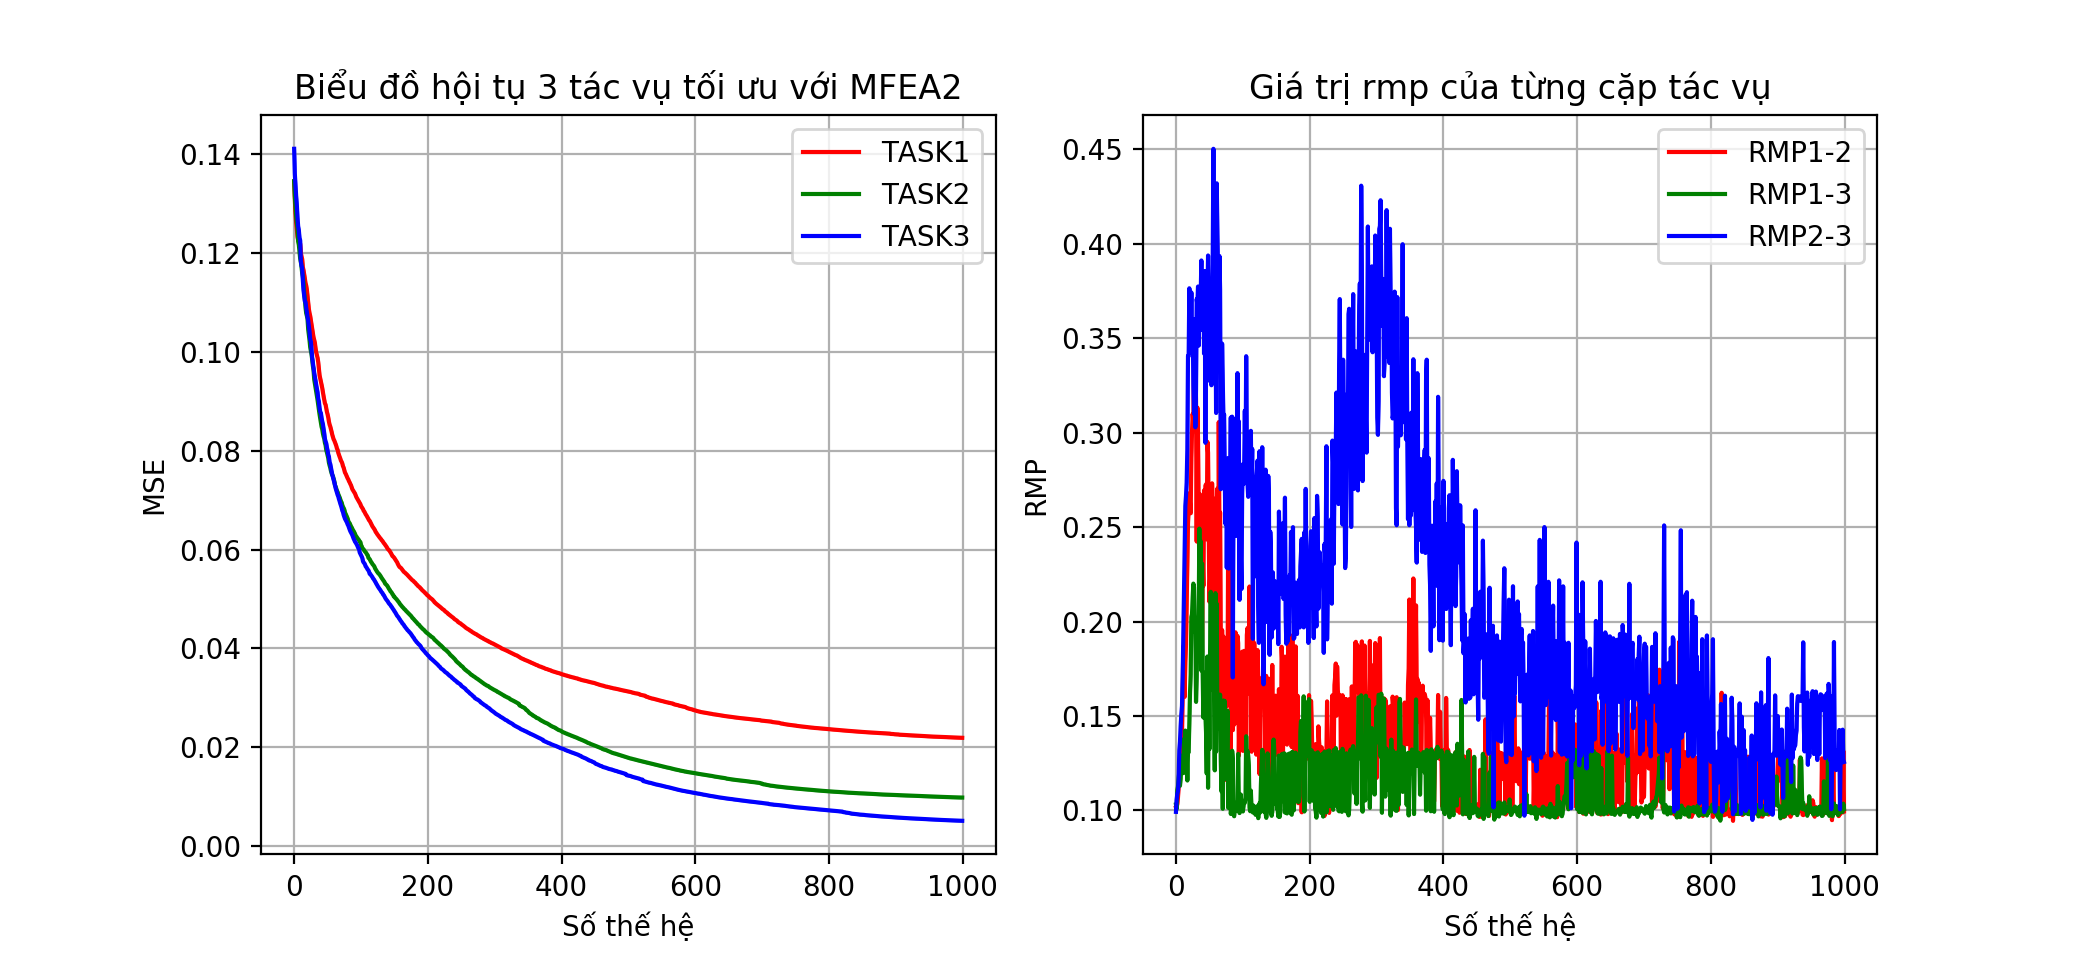
\includegraphics[width=\textwidth,height=\textheight,keepaspectratio]{thesis/images/results/nbit_1layer/4bit_rmp.png}}
    \label{fig:4bit_1layer}
    \caption{Bài 4bit: Biểu đồ hội tụ của từng tác vụ trên các thuật toán và biểu đồ phân tích MFEA-II theo giá trị rmp}

\end{figure}
\begin{figure}[H]
    \centering
    \scalebox{.7}{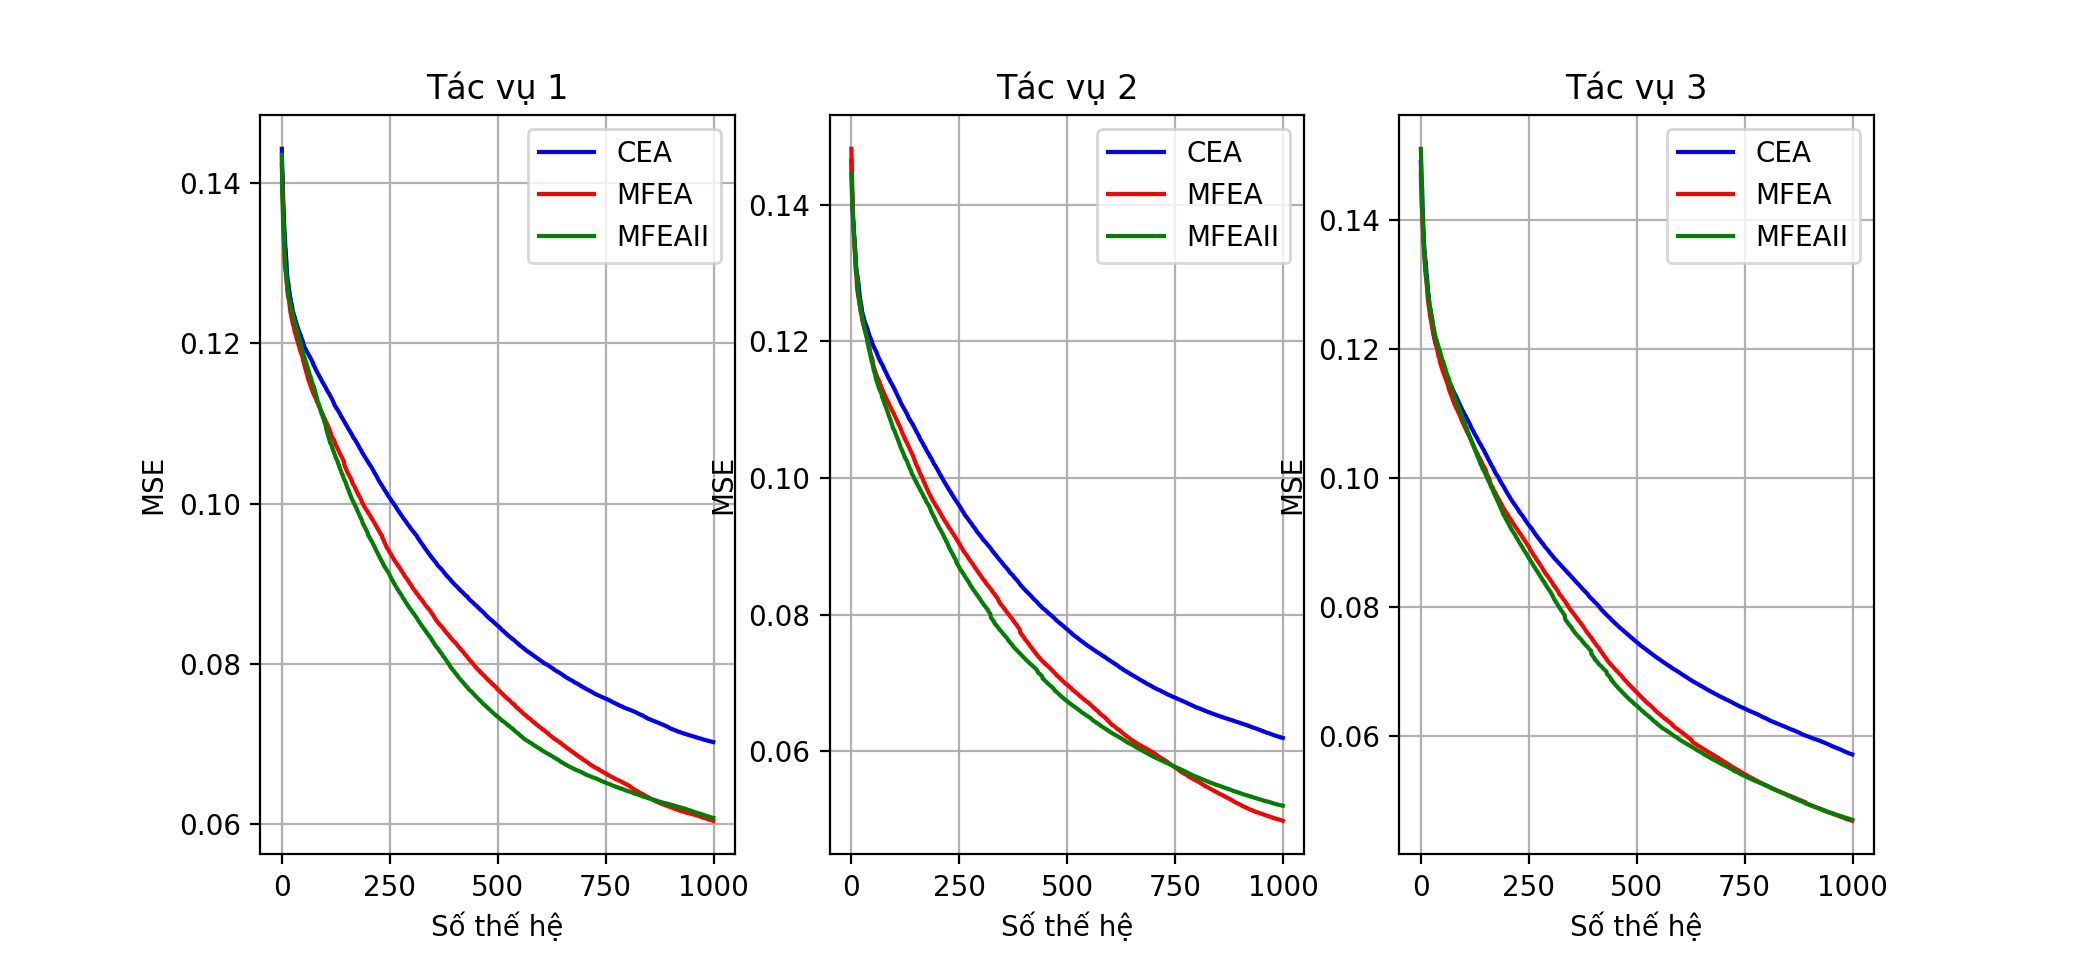
\includegraphics[width=\textwidth,height=\textheight,keepaspectratio]{thesis/images/results/nbit_1layer/6bit1_task.png}}
    \scalebox{.7}{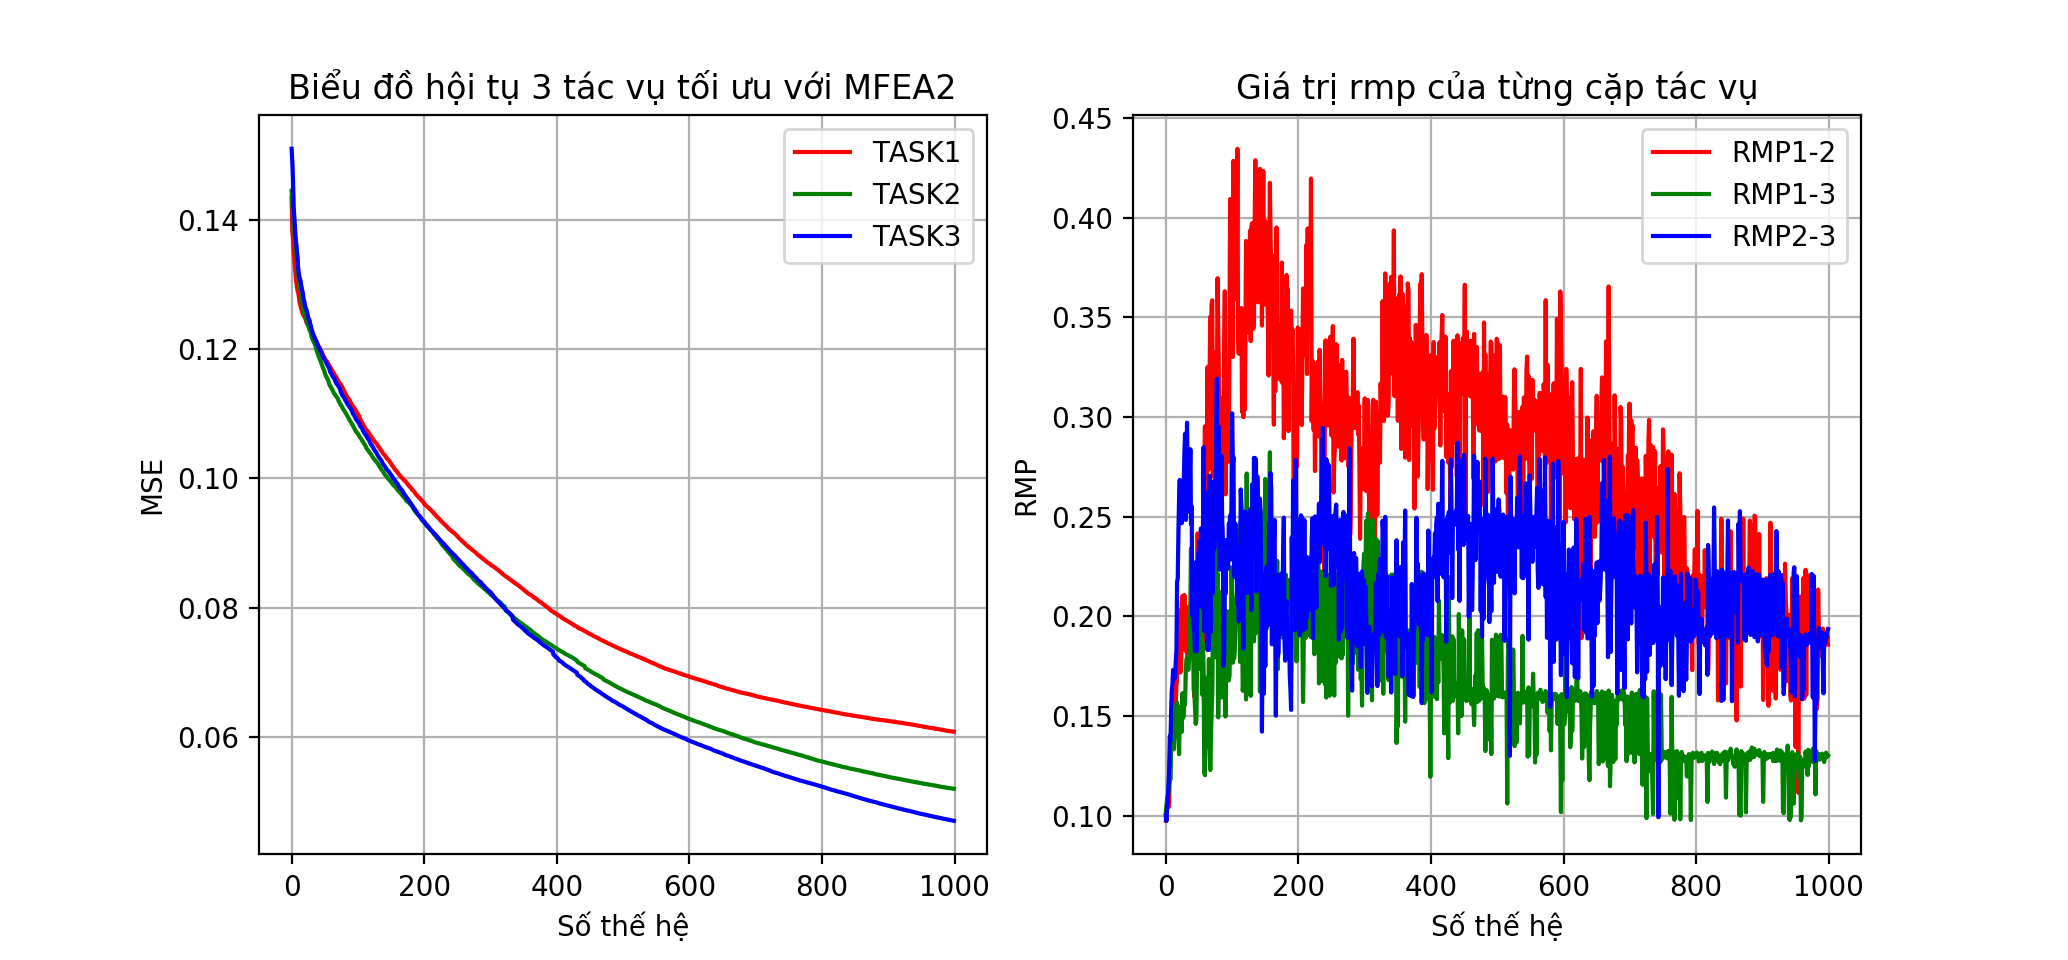
\includegraphics[width=\textwidth,height=\textheight,keepaspectratio]{thesis/images/results/nbit_1layer/6bit1_rmp.png}}
    \label{fig:6bit_1}
    \caption{Bài 6bit(5,6,7): Biểu đồ hội tụ của từng tác vụ trên các thuật toán và biểu đồ phân tích MFEA-II theo giá trị rmp}

\end{figure}
\begin{figure}[H]

    \centering
    \scalebox{.7}{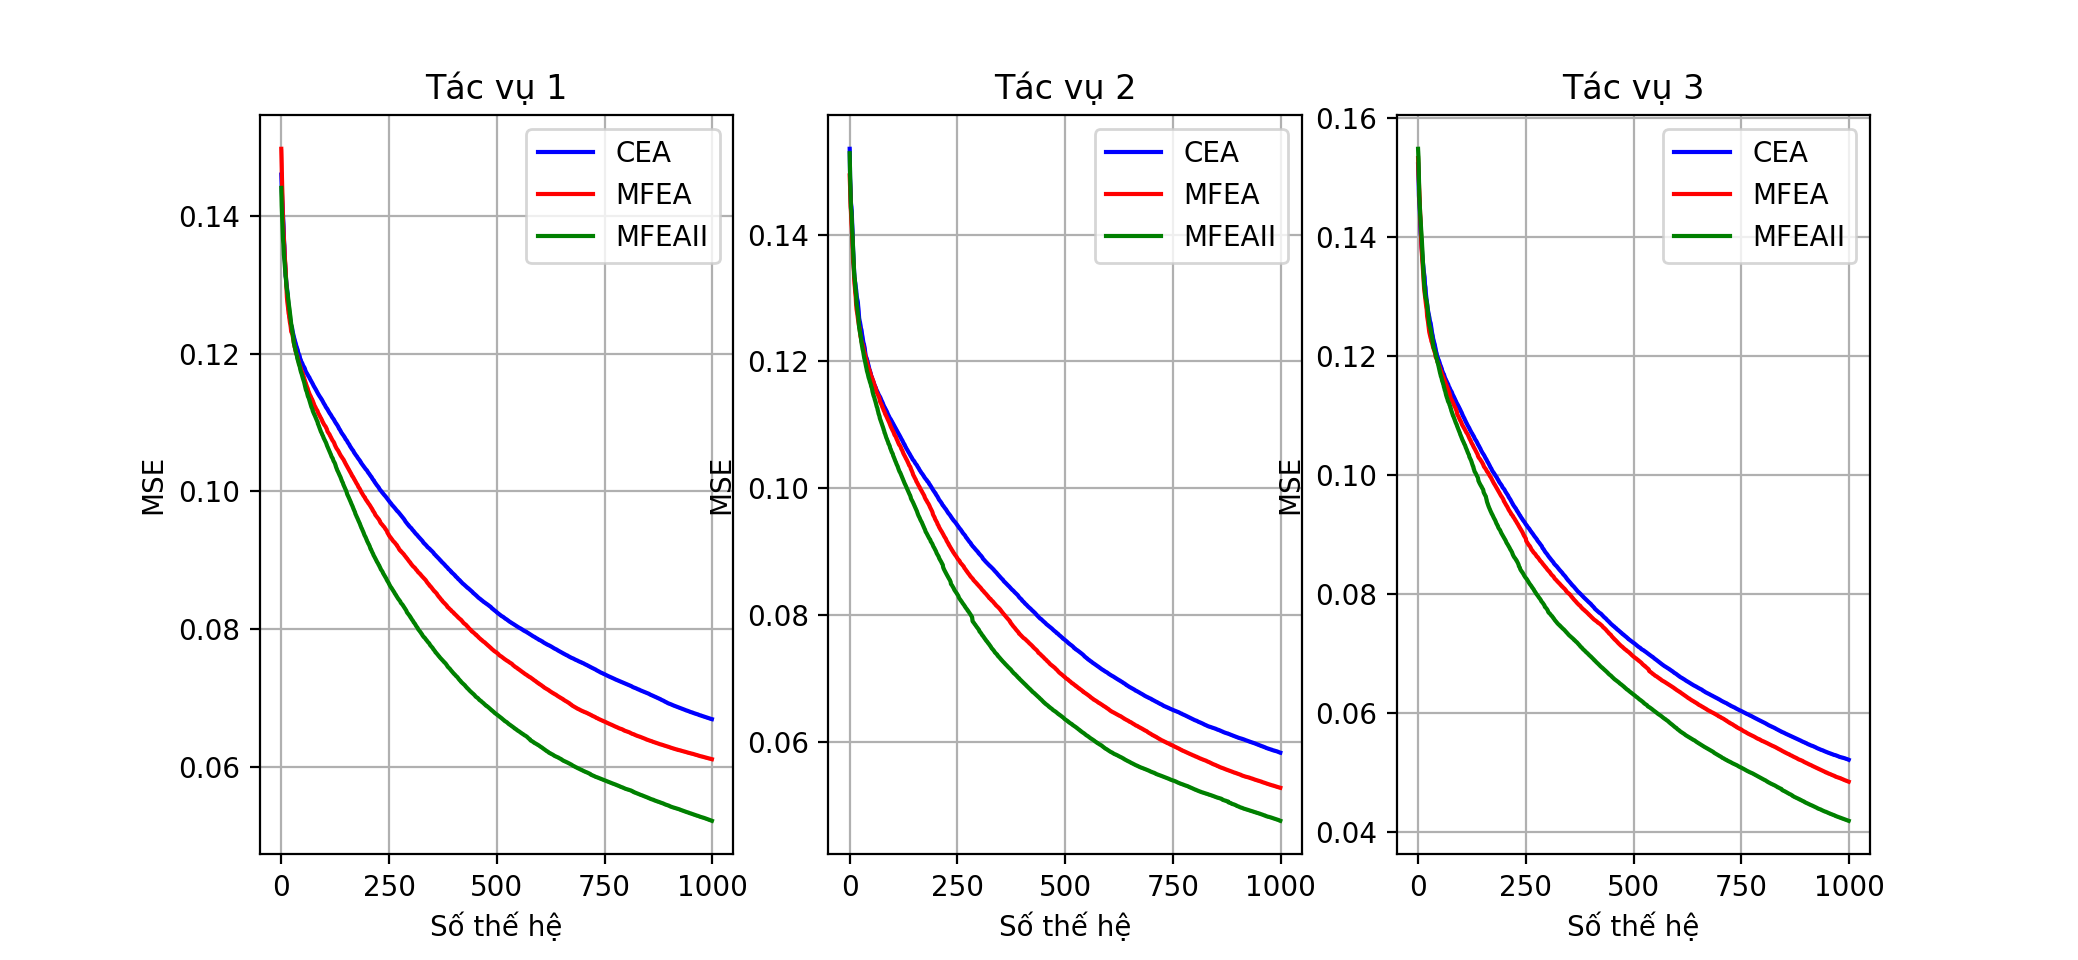
\includegraphics[width=\textwidth,height=\textheight,keepaspectratio]{thesis/images/results/nbit_1layer/6bit2_task.png}}
    \scalebox{.7}{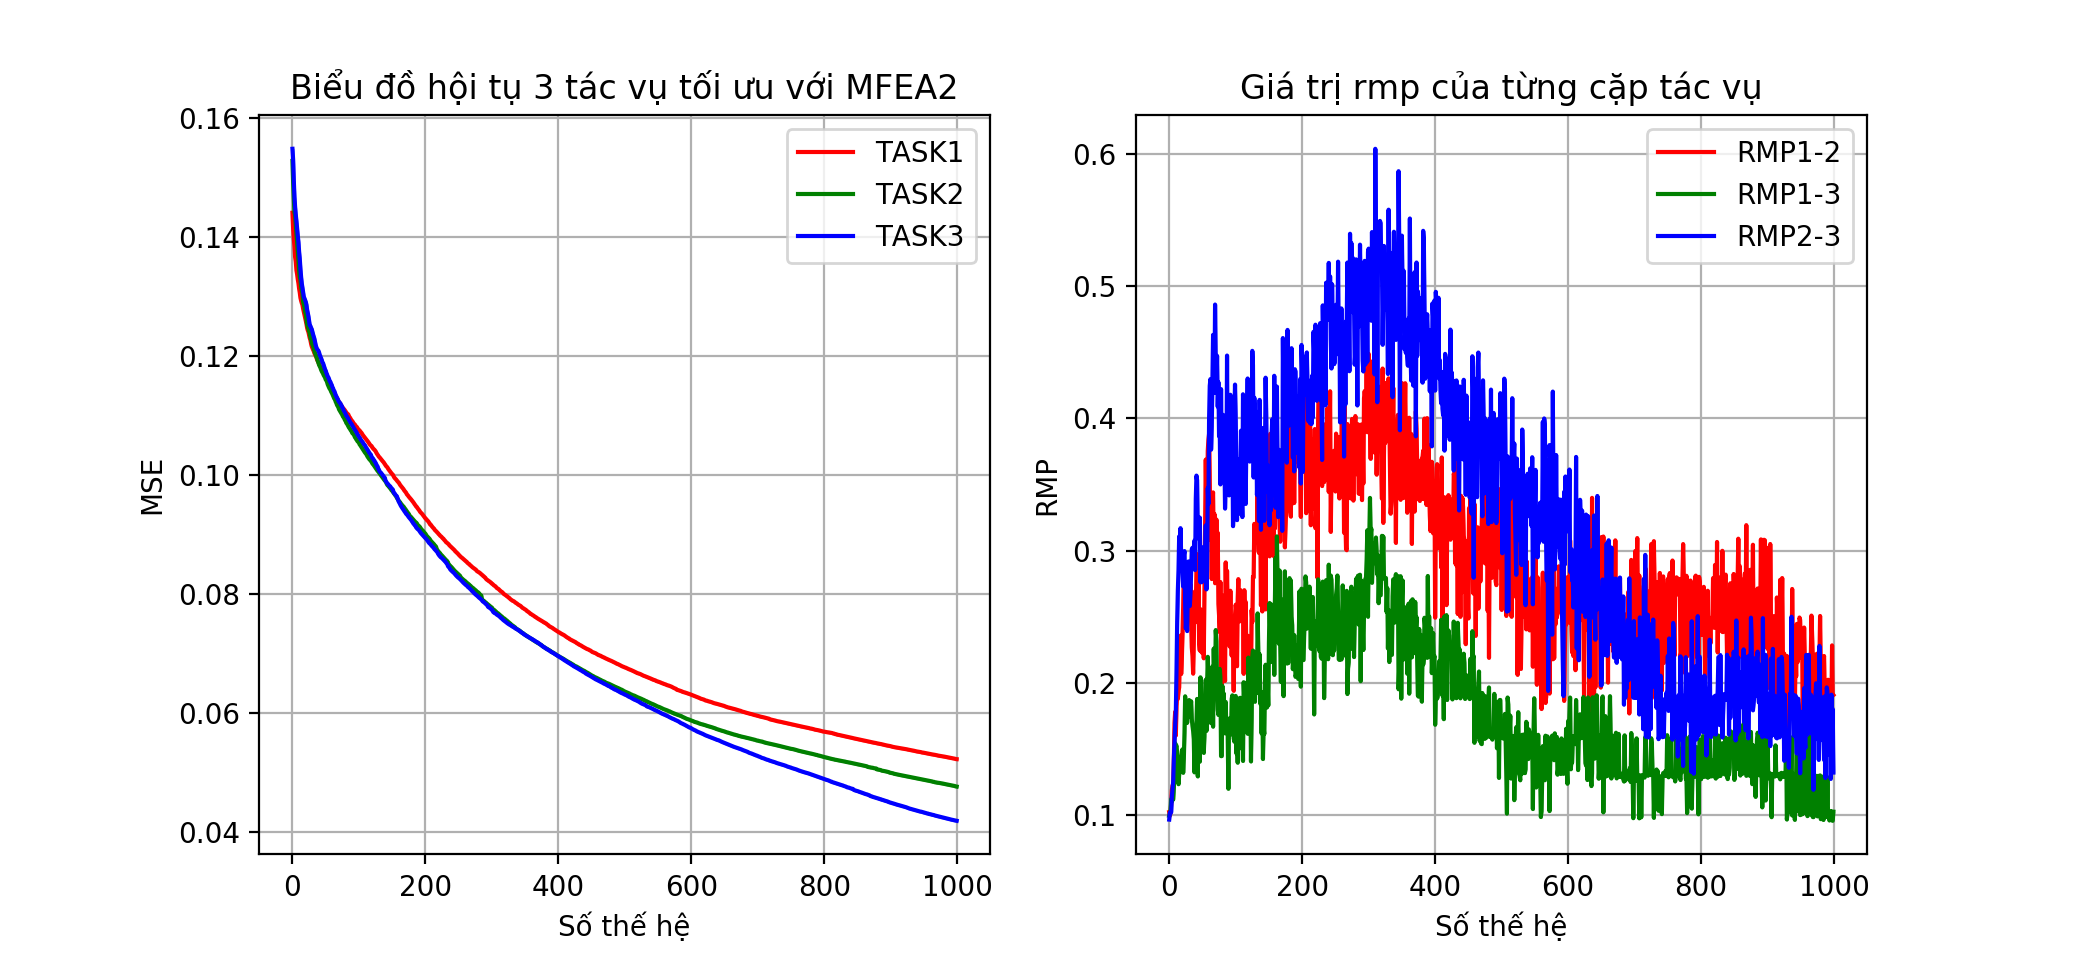
\includegraphics[width=\textwidth,height=\textheight,keepaspectratio]{thesis/images/results/nbit_1layer/6bit2_rmp.png}}
    \label{fig:6bit2_1layer}
        \caption{Bài 6bit(6,7,8): Biểu đồ hội tụ của từng tác vụ trên các thuật toán và biểu đồ phân tích MFEA-II theo giá trị rmp}

\end{figure}
\begin{figure}[H]
    \centering

    \scalebox{.7}{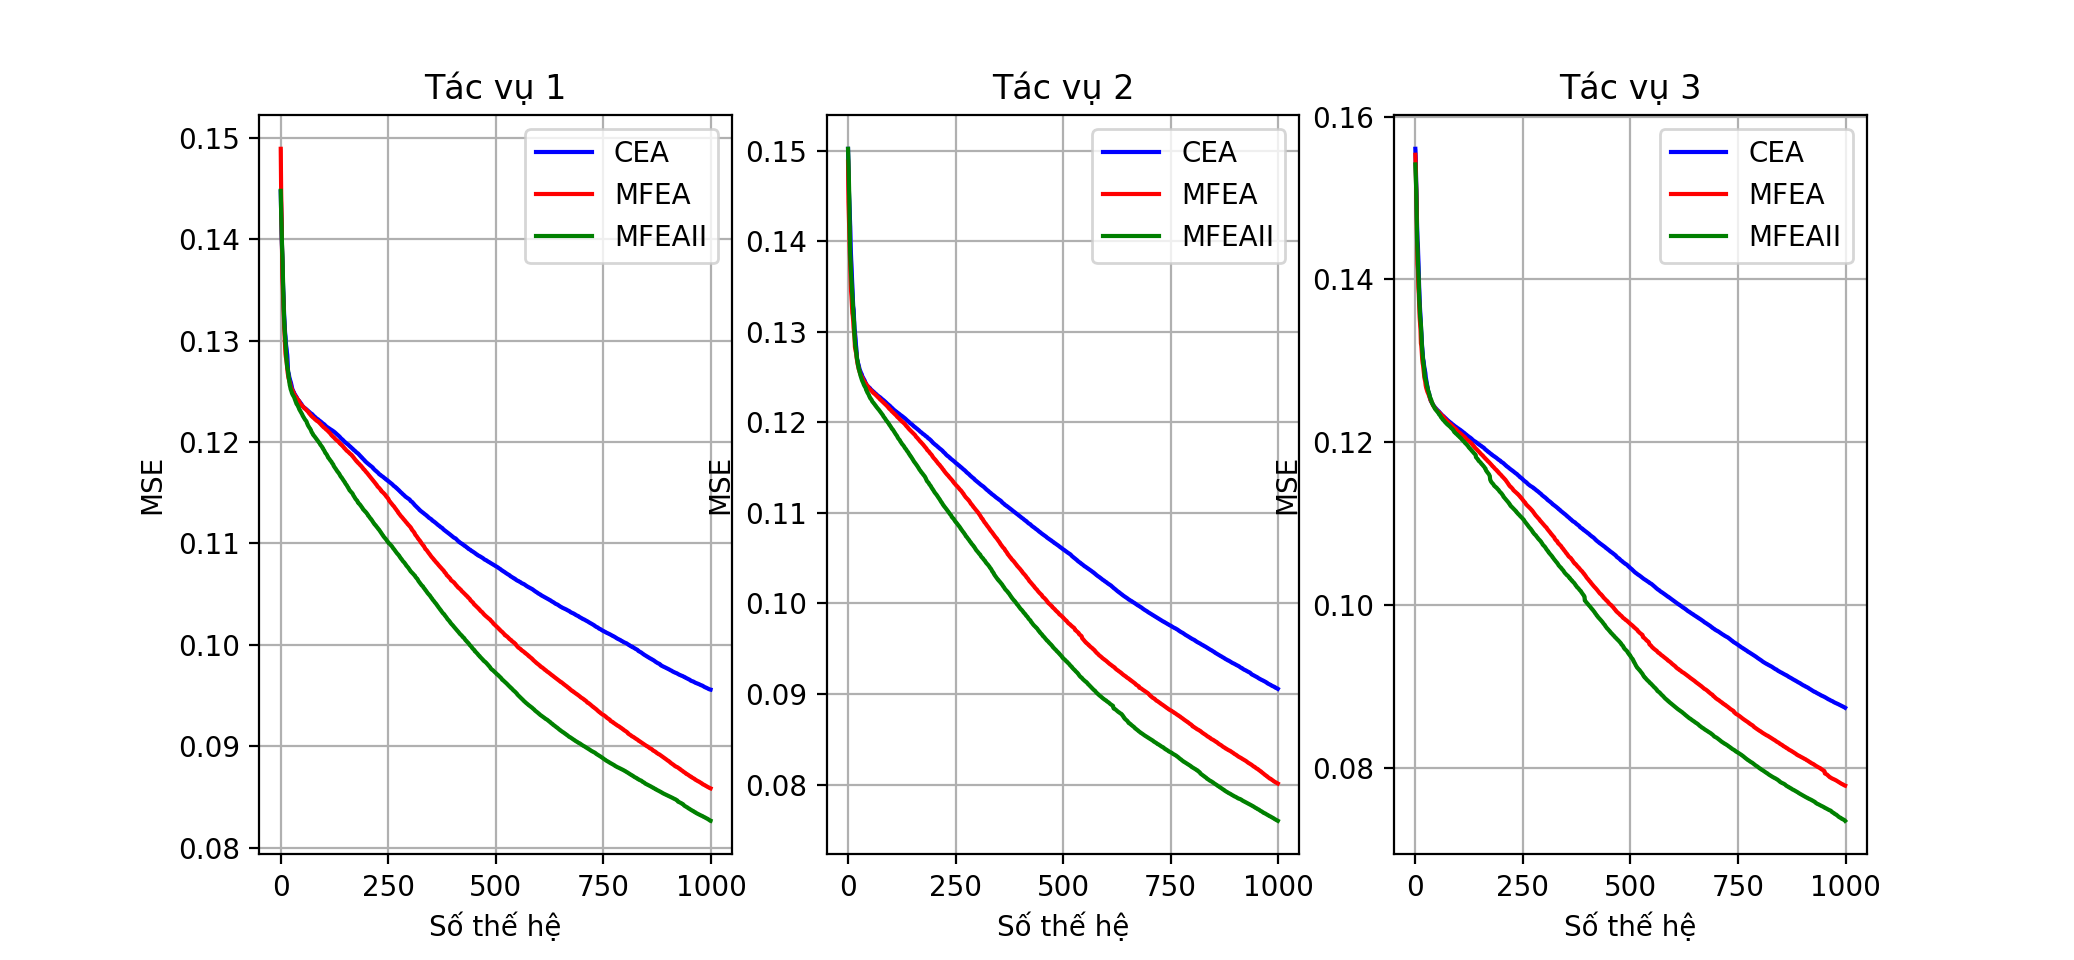
\includegraphics[width=\textwidth,height=\textheight,keepaspectratio]{thesis/images/results/nbit_1layer/8bit1_task.png}}
    \scalebox{.7}{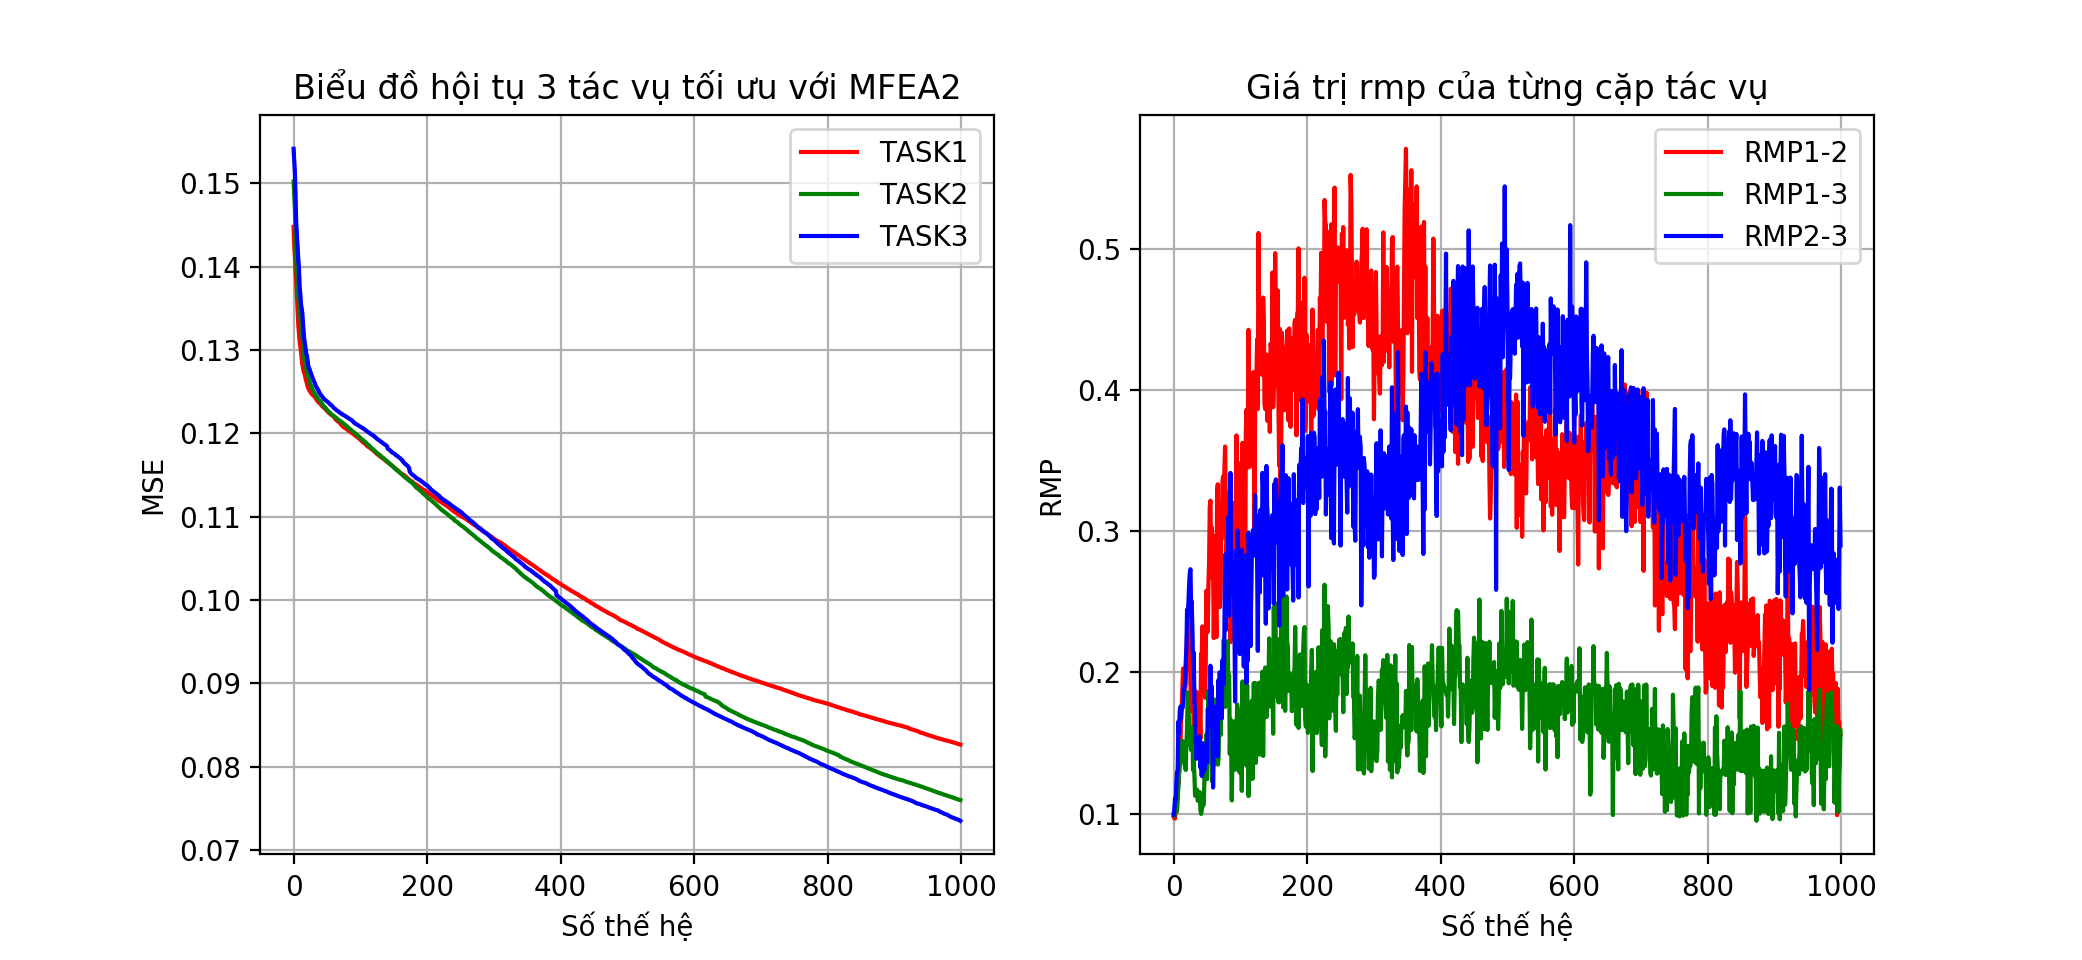
\includegraphics[width=\textwidth,height=\textheight,keepaspectratio]{thesis/images/results/nbit_1layer/8bit1_rmp.png}}
    \label{fig:8bit1_1layer}
    \caption{Bài 8bit(5,6,7):Biểu đồ hội tụ của từng tác vụ trên các thuật toán và biểu đồ phân tích MFEA-II theo giá trị rmp}

\end{figure}
\begin{figure}[H]
    \centering

    \scalebox{.7}{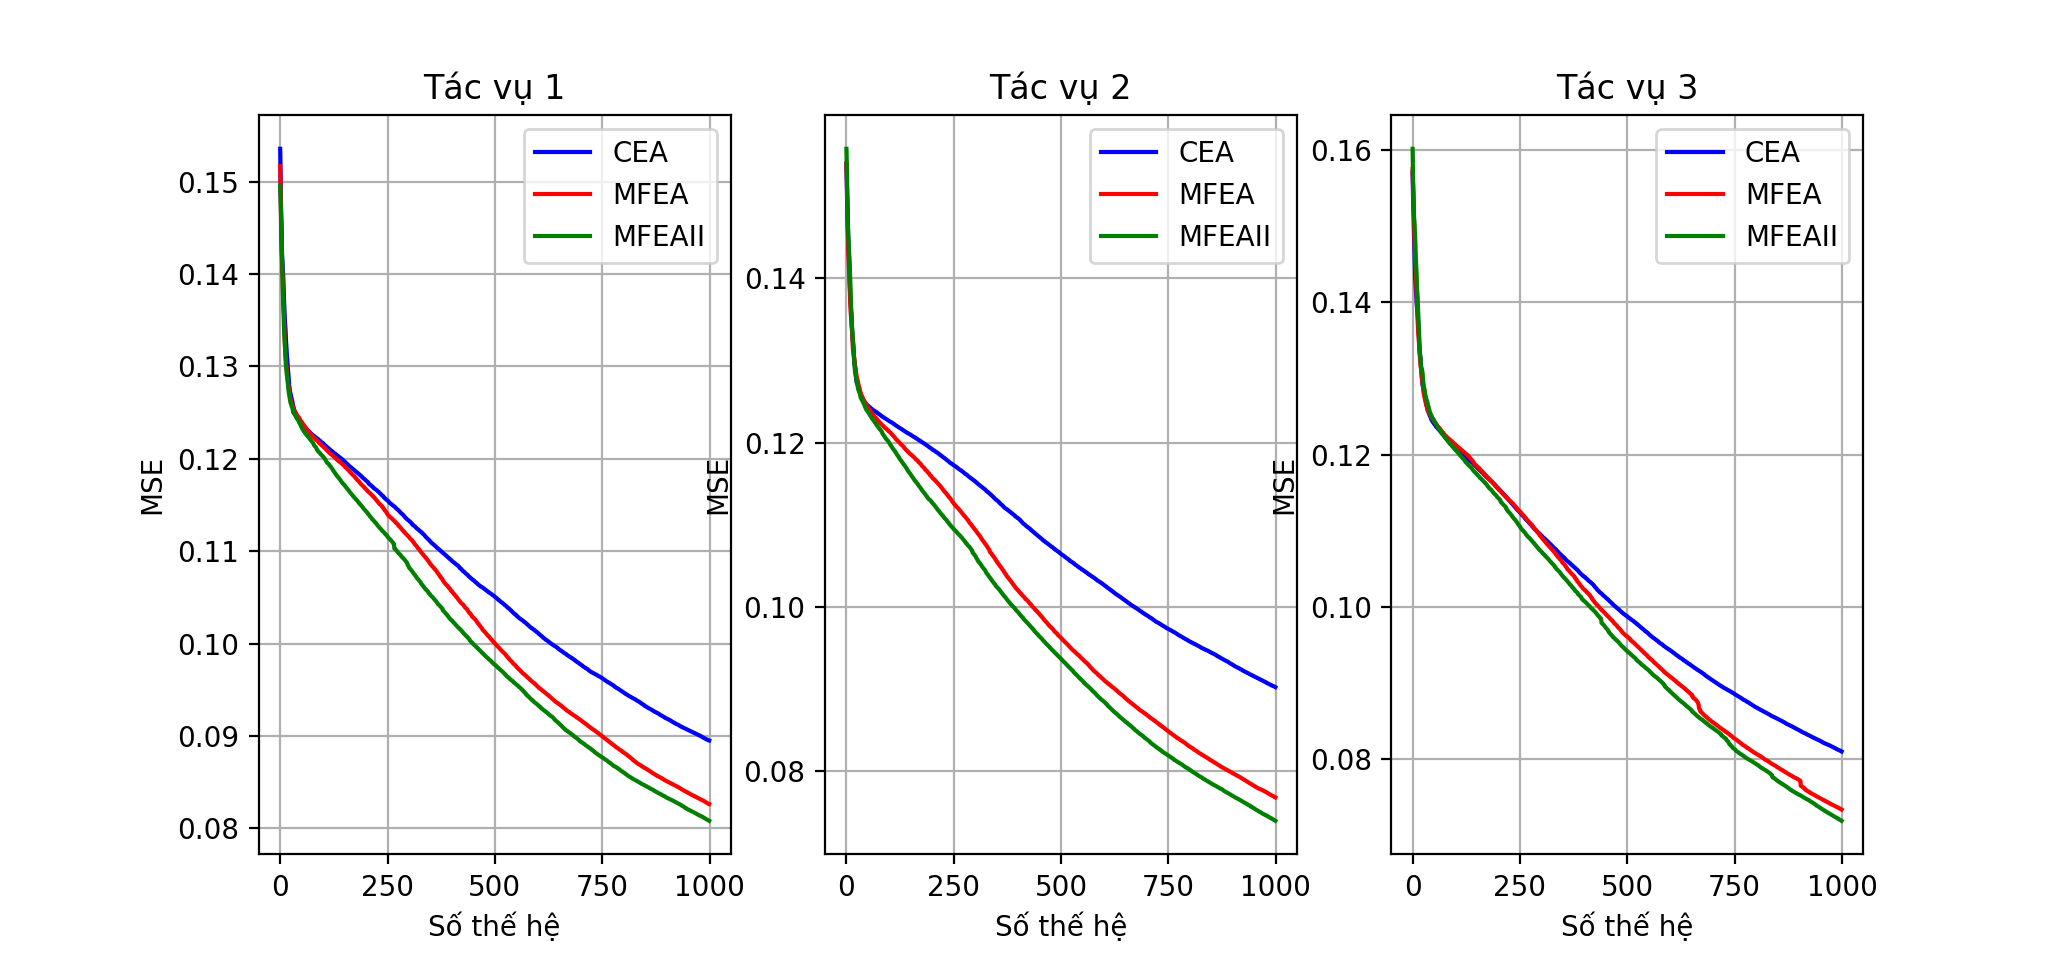
\includegraphics[width=\textwidth,height=\textheight,keepaspectratio]{thesis/images/results/nbit_1layer/8bit2_task.png}}
    \scalebox{.7}{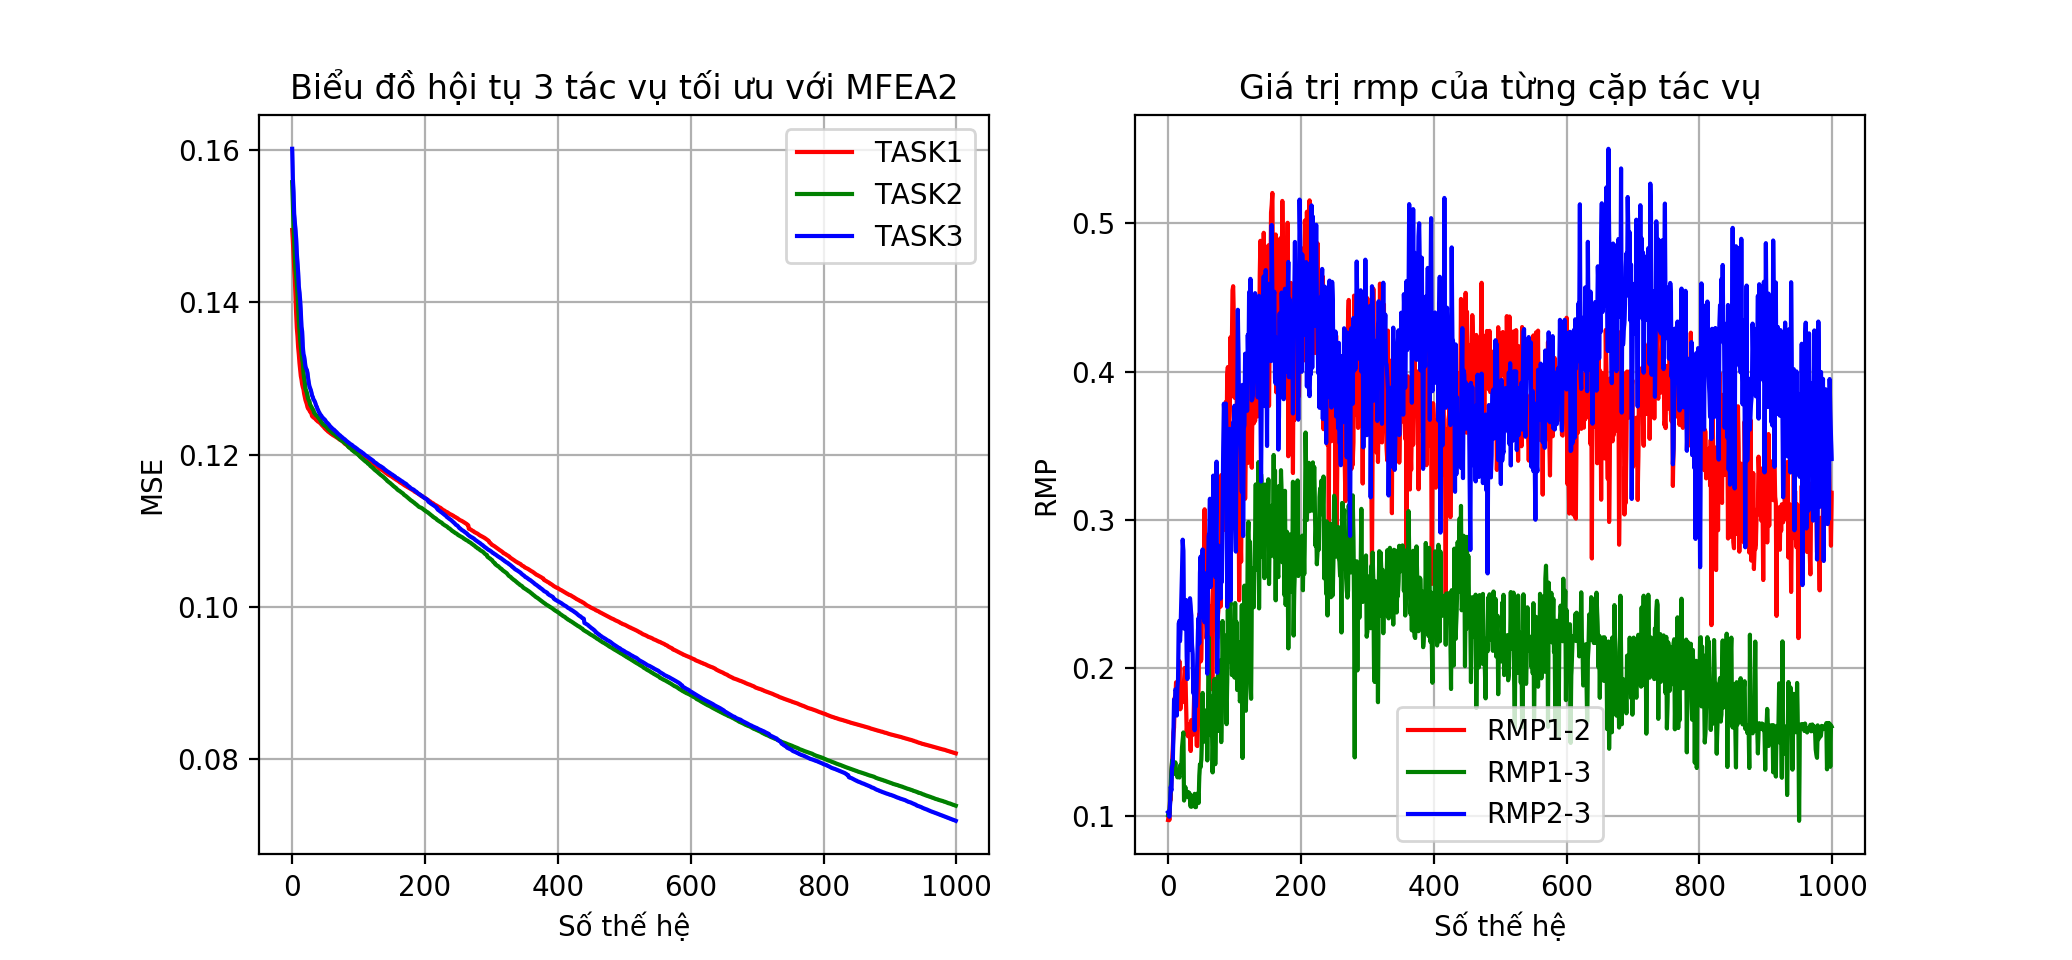
\includegraphics[width=\textwidth,height=\textheight,keepaspectratio]{thesis/images/results/nbit_1layer/8bit2_rmp.png}}
    \label{fig:8bit2_1layer}
    \caption{Bài 8bit(6,7,8): Biểu đồ hội tụ của từng tác vụ trên các thuật toán và biểu đồ phân tích MFEA-II theo giá trị rmp}

\end{figure}

\subsubsection{Bảng kết quả thực nghiệm - mạng neural cùng độ sâu 2 lớp ẩn}
\begin{table} [H]
    \begin{center}
    \caption{Kết quả thực nghiệm huấn luyện ANN 2 lớp ẩn}
    \begin{tabular}{|c|c|c|c|c|}
    \hline
    \multirow{1}{*}{\textbf{Bài toán}} &
    \multirow{1}{*}{\textbf{Method}} & \multicolumn{1}{c|}{\textbf{Tác vụ 1}} & \multicolumn{1}{c|}{\textbf{Tác vụ 2}} & \multicolumn{1}{c|}{\textbf{Tác vụ 3}} \\ \hline
    \multirow{3}{*} 
    {8-bit} &
    CEA & $0.075 \pm 0.012865$ & $0.0713 \pm 0.013116$ & $0.0718 \pm 0.012432$  \\
    & MFEA-I & $0.0738 \pm 0.012508$ & $0.0684 \pm 0.013252$ & $0.0669 \pm 0.015076$   \\
    & MFEA-II & $\mathbf{0.0705 \pm 0.012856}$ & $\mathbf{0.0624 \pm 0.011079}$ & $\mathbf{0.0595 \pm 0.011252}$\\\hline
    \multirow{3}{*} 
    {9-bit} &
    CEA & $0.0826 \pm 0.010588$ & $0.0751 \pm 0.014406$ & $0.0785 \pm 0.010766$  \\
    & MFEA-I & $0.0827 \pm 0.010438$ & $0.0762 \pm 0.009495$ & $0.0737 \pm 0.009766$ \\
    & MFEA-II & $\mathbf{0.0795 \pm 0.012865}$ & $\mathbf{0.0705 \pm 0.009581}$ & $\mathbf{0.0685 \pm 0.011156}$ \\\hline
    \multirow{3}{*} 
    {10-bit} &
    CEA & $0.0853 \pm 0.01105$ & $0.0862 \pm 0.008326$ & $0.0856 \pm 0.008919$  \\
    & MFEA-I  & $0.0855 \pm 0.012229$ & $\mathbf{0.0782 \pm 0.009659}$ & $\mathbf{0.0752 \pm 0.009681}$ \\
    & MFEA-II & $\mathbf{0.0833 \pm 0.010222}$ & $0.0791 \pm 0.009846$ & $0.0762 \pm 0.010419$ \\\hline
    \end{tabular}
    \end{center}

    \label{tab:result:nbit}
\end{table}

\subsubsection{Biểu đồ hội tụ - Mạng neural cùng độ sâu 2 lớp ẩn}
\begin{figure}[h!]
    \centering
    \scalebox{.7}{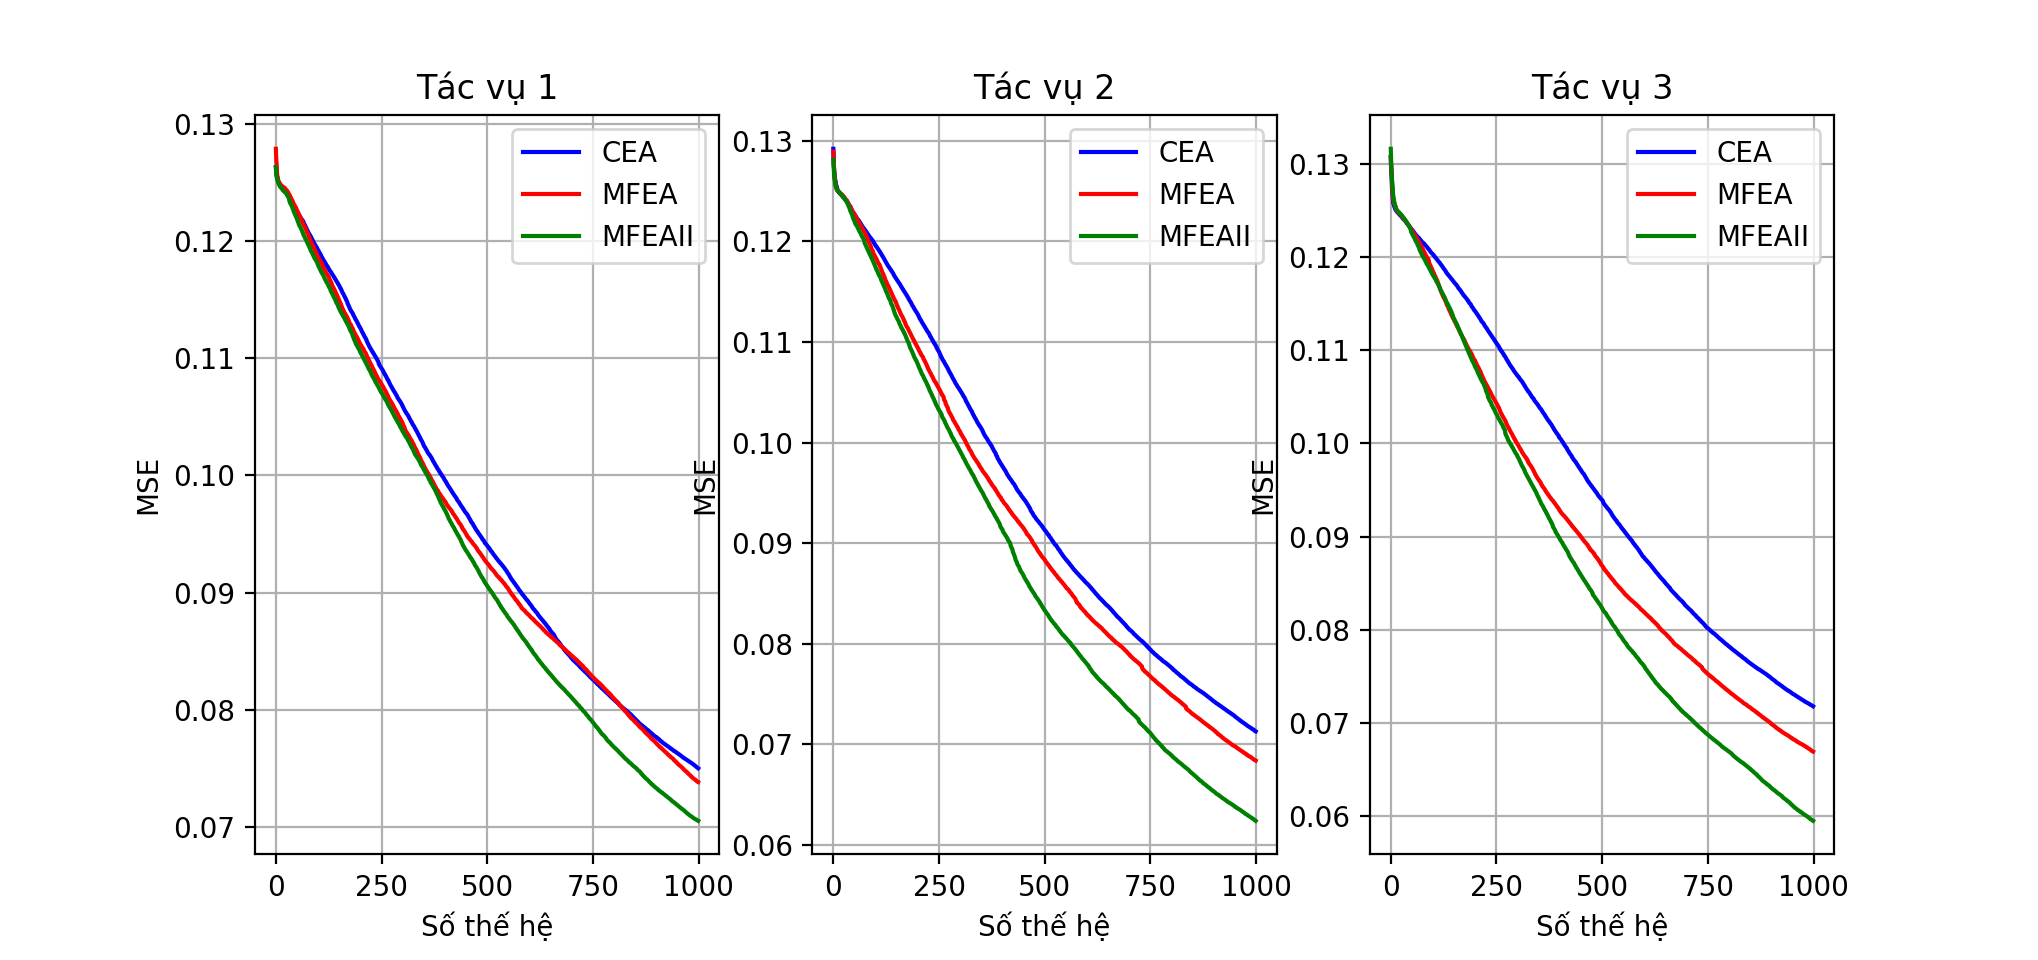
\includegraphics[width=\textwidth,height=\textheight,keepaspectratio]{thesis/images/results/nbit_2layer/8bit1_task.png}}
    \scalebox{.7}{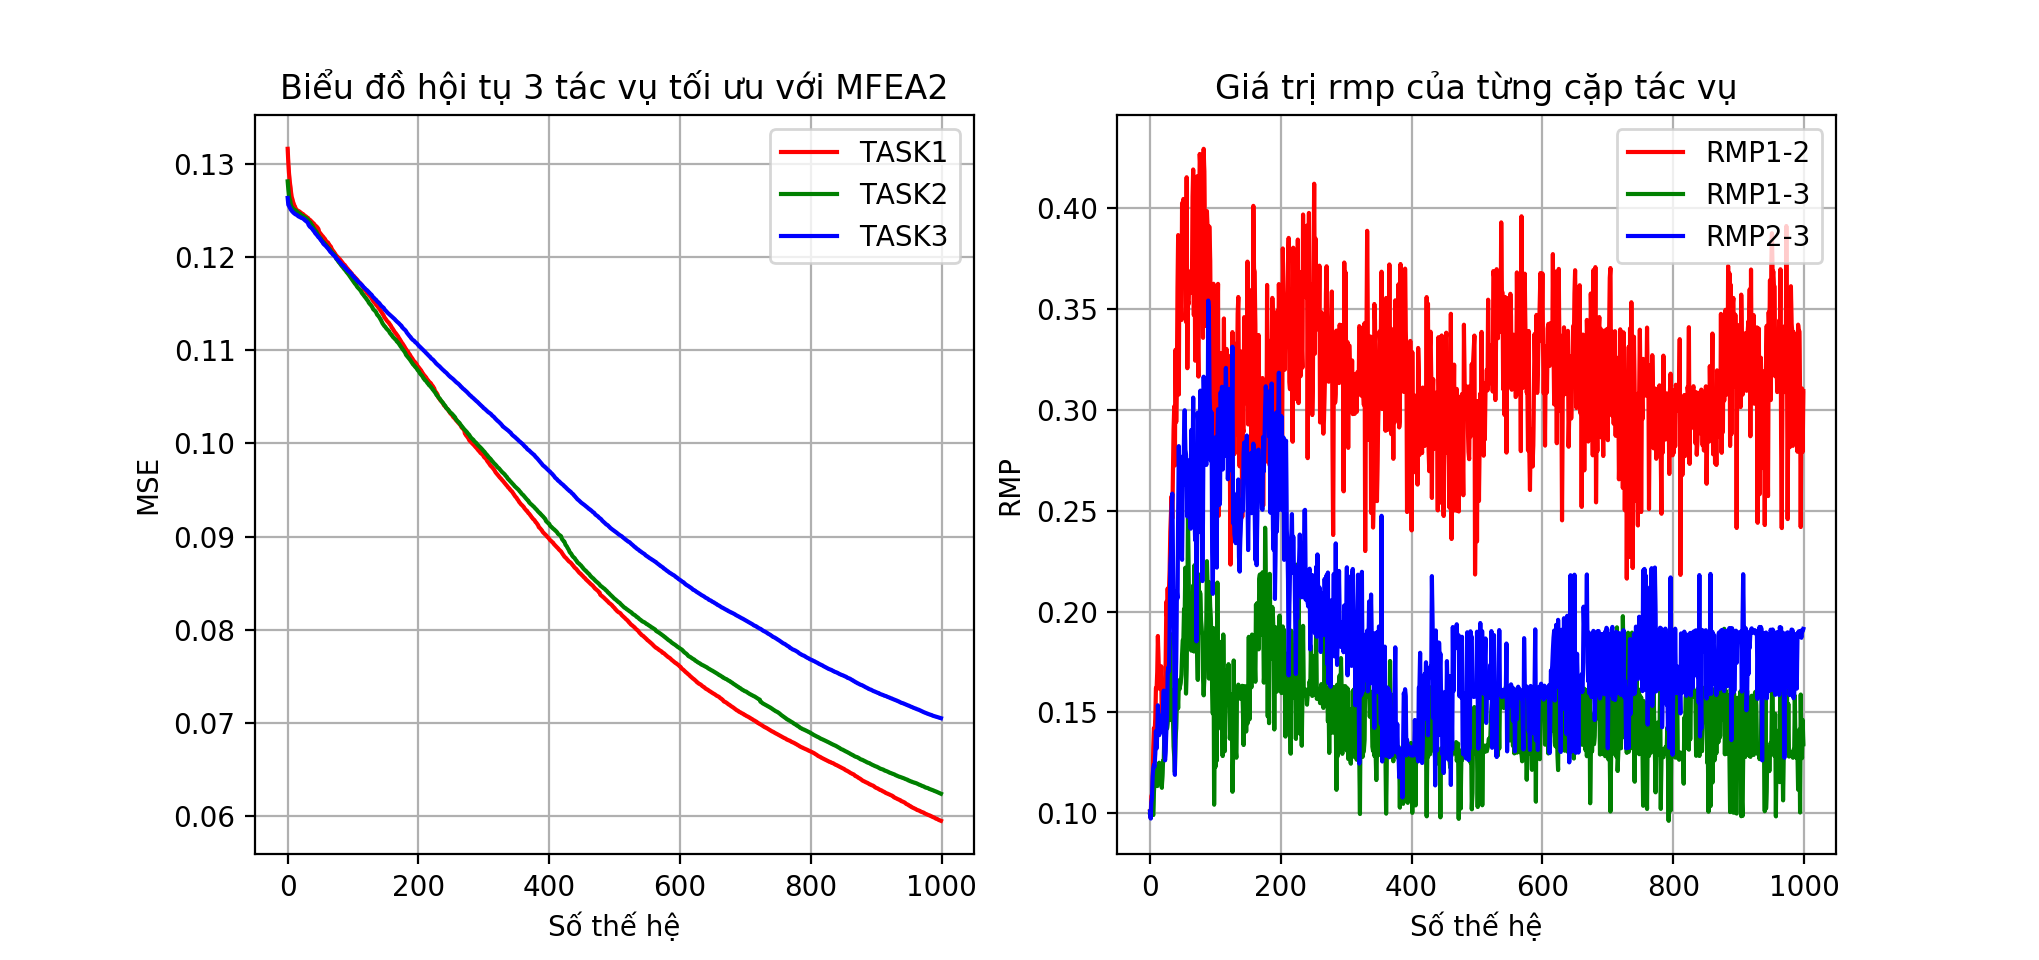
\includegraphics[width=\textwidth,height=\textheight,keepaspectratio]{thesis/images/results/nbit_2layer/8bit1_rmp.png}}
    \caption{Bài 8bit: Biểu đồ hội tụ của từng tác vụ trên các thuật toán và biểu đồ phân tích MFEA-II theo giá trị rmp}
    \label{fig:8bit_2layer}
\end{figure}
\begin{figure}[h!]
    \centering
    \scalebox{.7}{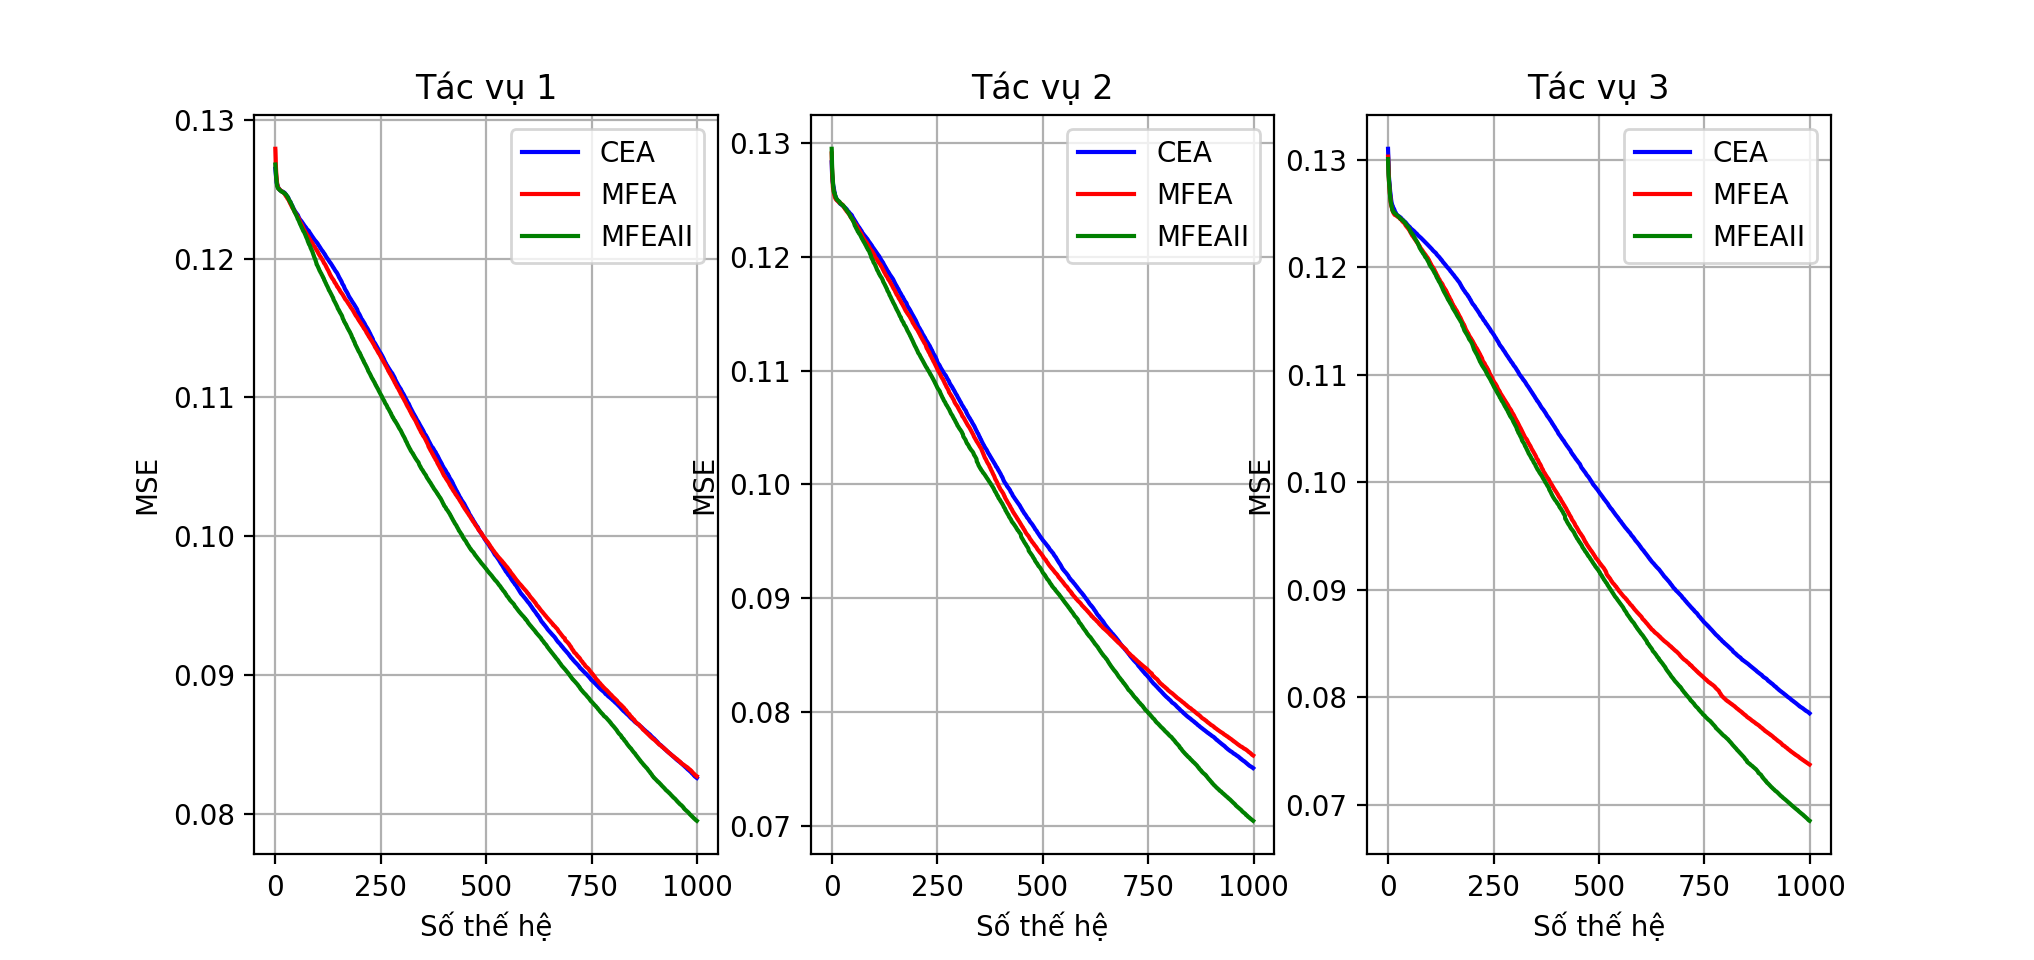
\includegraphics[width=\textwidth,height=\textheight,keepaspectratio]{thesis/images/results/nbit_2layer/9bit1_task.png}}
    \scalebox{.7}{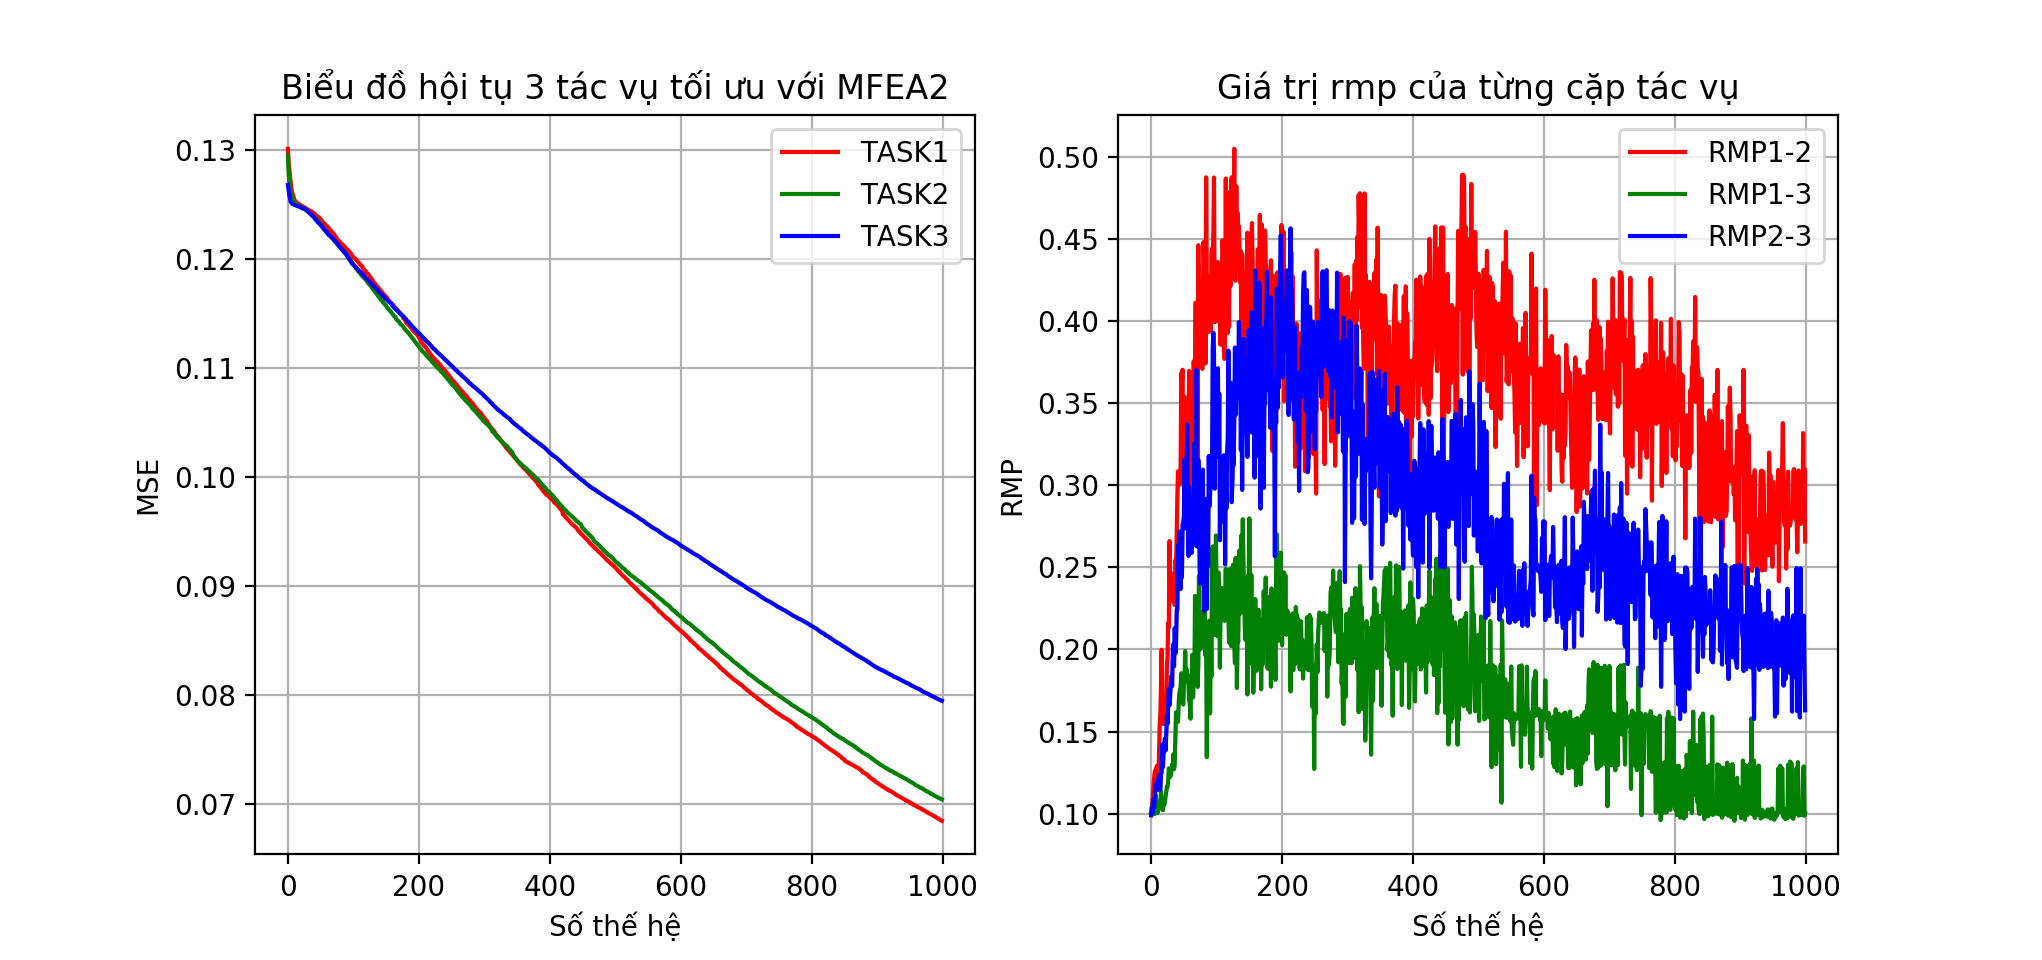
\includegraphics[width=\textwidth,height=\textheight,keepaspectratio]{thesis/images/results/nbit_2layer/9bit1_rmp.png}}
    \caption{Bài 9bit: Biểu đồ hội tụ của từng tác vụ trên các thuật toán và biểu đồ phân tích MFEA-II theo giá trị rmp}
    \label{fig:9bit_2layer}
\end{figure}
\begin{figure}[h!]
    \centering
    \scalebox{.7}{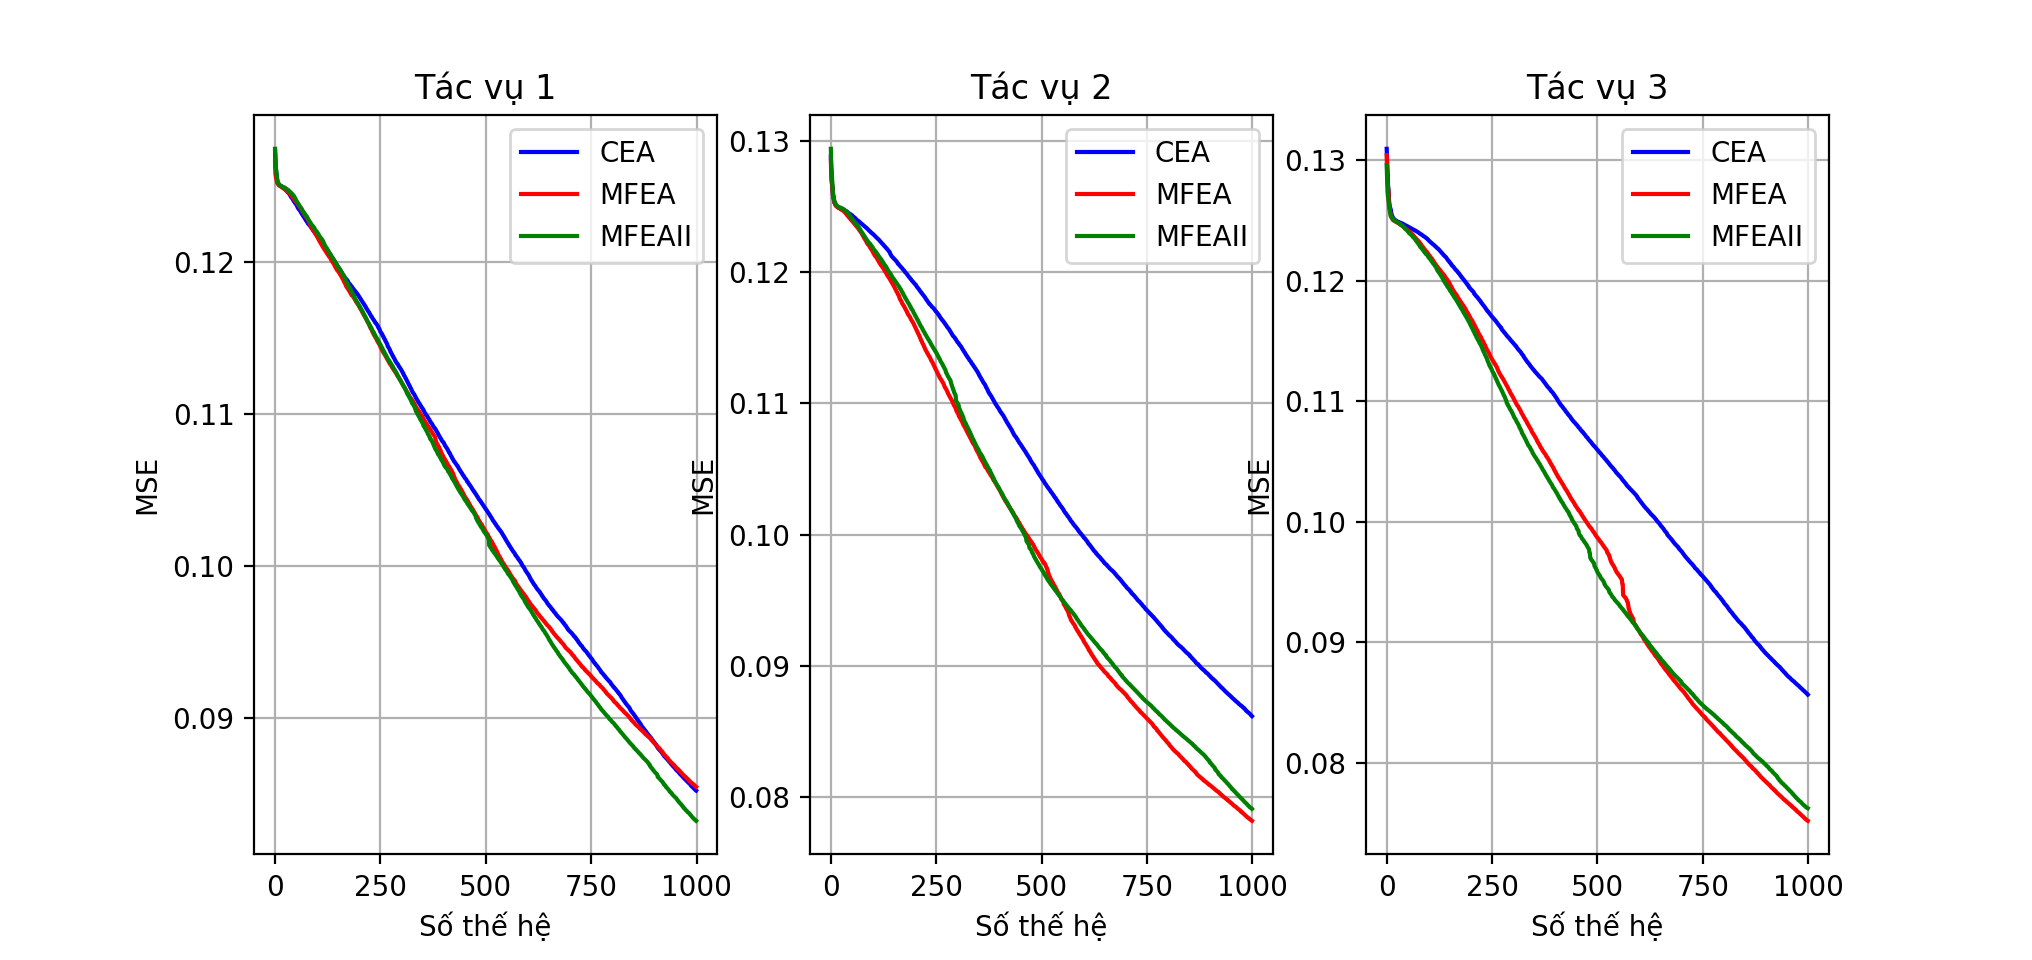
\includegraphics[width=\textwidth,height=\textheight,keepaspectratio]{thesis/images/results/nbit_2layer/10bit1_task.png}}
    \scalebox{.7}{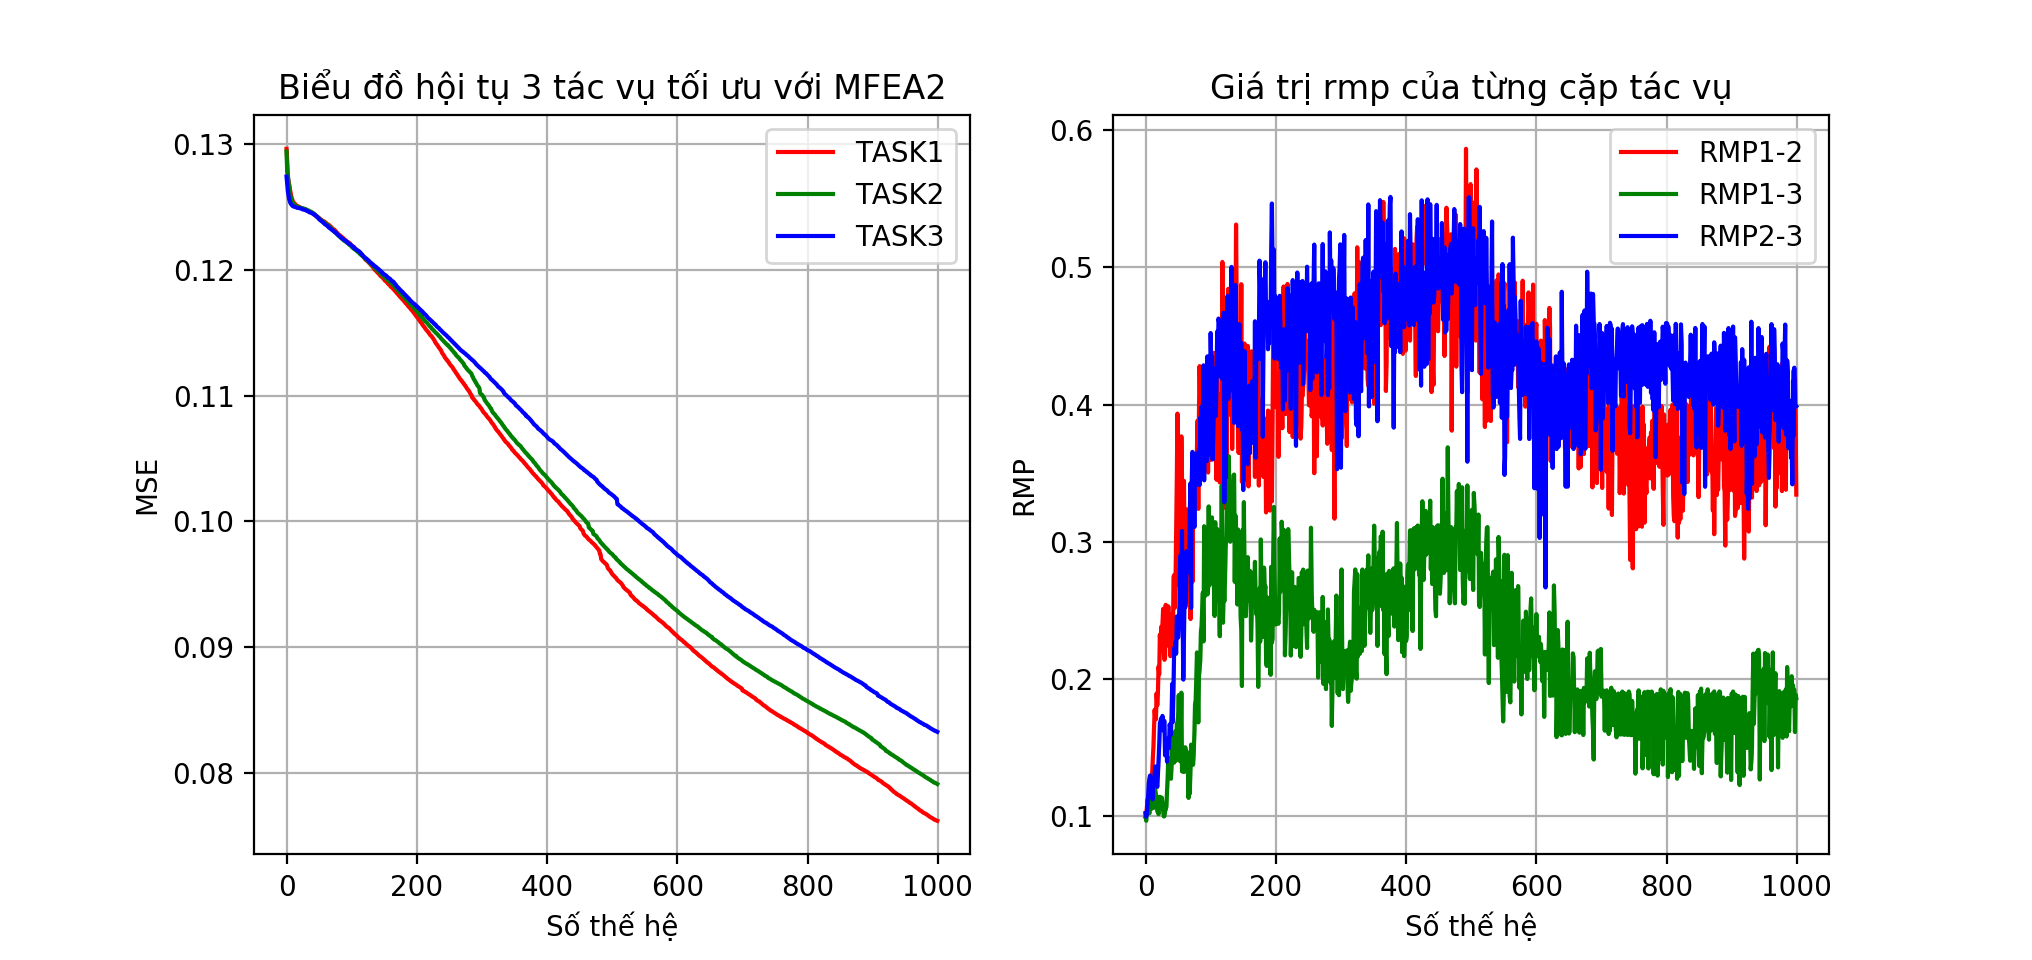
\includegraphics[width=\textwidth,height=\textheight,keepaspectratio]{thesis/images/results/nbit_2layer/10bit1_rmp.png}}
    \caption{Bài 10bit: Biểu đồ hội tụ của từng tác vụ trên các thuật toán và biểu đồ phân tích MFEA-II theo giá trị rmp}
    \label{fig:10bit_2layer}
\end{figure}
\newpage

\subsubsection{Bảng kết quả thực nghiệm - mạng neural khác độ sâu}
\begin{table} [H]
    \begin{center}
    \caption{Kết quả huấn luyện ANN khác độ sâu}
    \begin{tabular}{|c|c|c|c|c|}
    \hline
    \multirow{1}{*}{\textbf{Bài toán}} &
    \multirow{1}{*}{\textbf{Method}} & \multicolumn{1}{c|}{\textbf{Tác vụ 1}} & \multicolumn{1}{c|}{\textbf{Tác vụ 2}} & \multicolumn{1}{c|}{\textbf{Tác vụ 3}} \\ \hline
    \multirow{3}{*} 
    {8-bit} &
    CEA & $0.0789 \pm 0.0172$ & $0.0815 \pm 0.0136$ & $\mathbf{0.0794 \pm 0.0156}$ \\
    & MFEA-I & $0.0778 \pm 0.0153$ & $0.0805 \pm 0.0142$ & $0.0814 \pm 0.0119$  \\
    & MFEA-II & $\mathbf{0.0721} \pm 0.0148$ & $\mathbf{0.0759 \pm 0.015}$ & $0.0822 \pm 0.0143$\\\hline
    \multirow{3}{*} 
    {9-bit} &
    CEA & $0.0843 \pm 0.0154$ & $0.0869 \pm 0.0141$ & $0.086 \pm 0.0128$  \\
    & MFEA-I & $0.0844 \pm 0.0124$ & $\mathbf{0.0795 \pm 0.0144}$ & $\mathbf{0.081 \pm 0.0134}$ \\
    & MFEA-II & $\mathbf{0.0828 \pm 0.0129}$ & $0.0818 \pm 0.0131$ & $0.0864 \pm 0.0147$ \\\hline
    \multirow{3}{*} 
    {10-bit} &
    CEA & $0.089 \pm 0.0131$ & $0.0922 \pm 0.0164$ & $0.0928 \pm 0.0124$  \\
    & MFEA-I  & $0.0879 \pm 0.0091$ & $0.0888 \pm 0.0124$ & $\mathbf{0.0873 \pm 0.0111}$ \\
    & MFEA-II & $\mathbf{0.0867 \pm 0.0079}$ & $\mathbf{0.0862 \pm 0.0103}$ & $0.0905 \pm 0.0104$ \\\hline
    \end{tabular}
    \end{center}
    \label{tab:result:nbit}

\end{table}

\subsubsection{Biểu đồ hội tụ - mạng neural khác độ sâu}

\begin{figure}[h!]
    \centering
    \scalebox{.57}{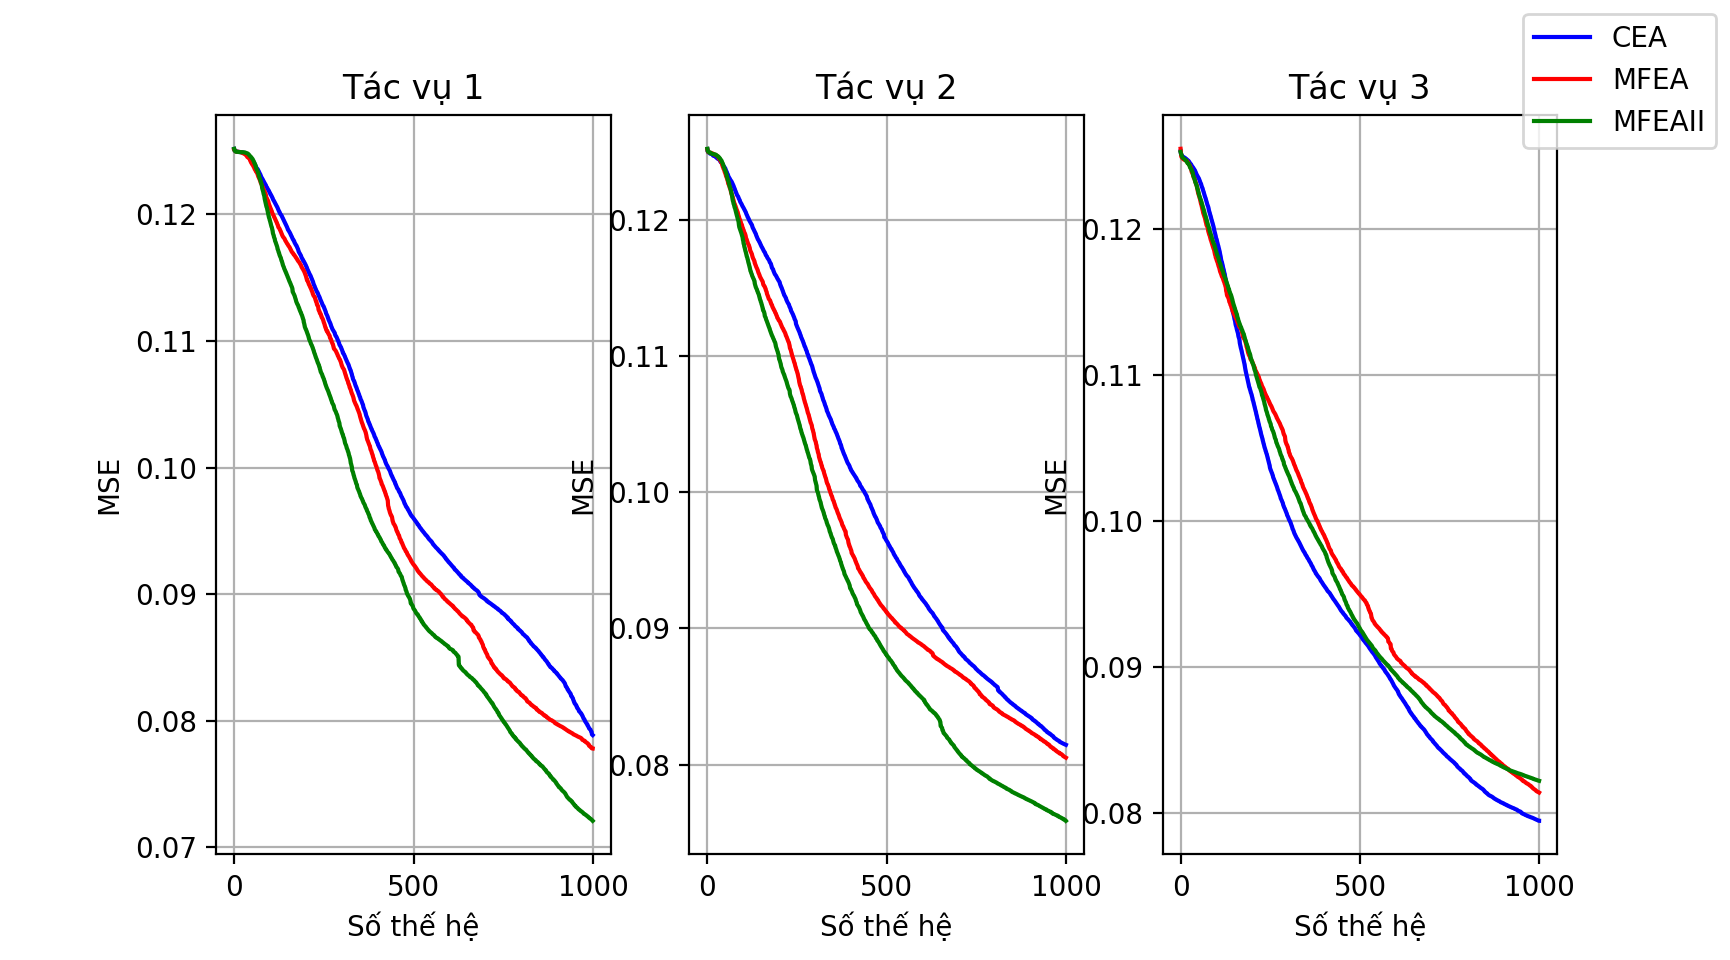
\includegraphics[width=\textwidth,height=\textheight,keepaspectratio]{thesis/images/results/multilayers/8bit2_task.png}}
    \scalebox{.57}{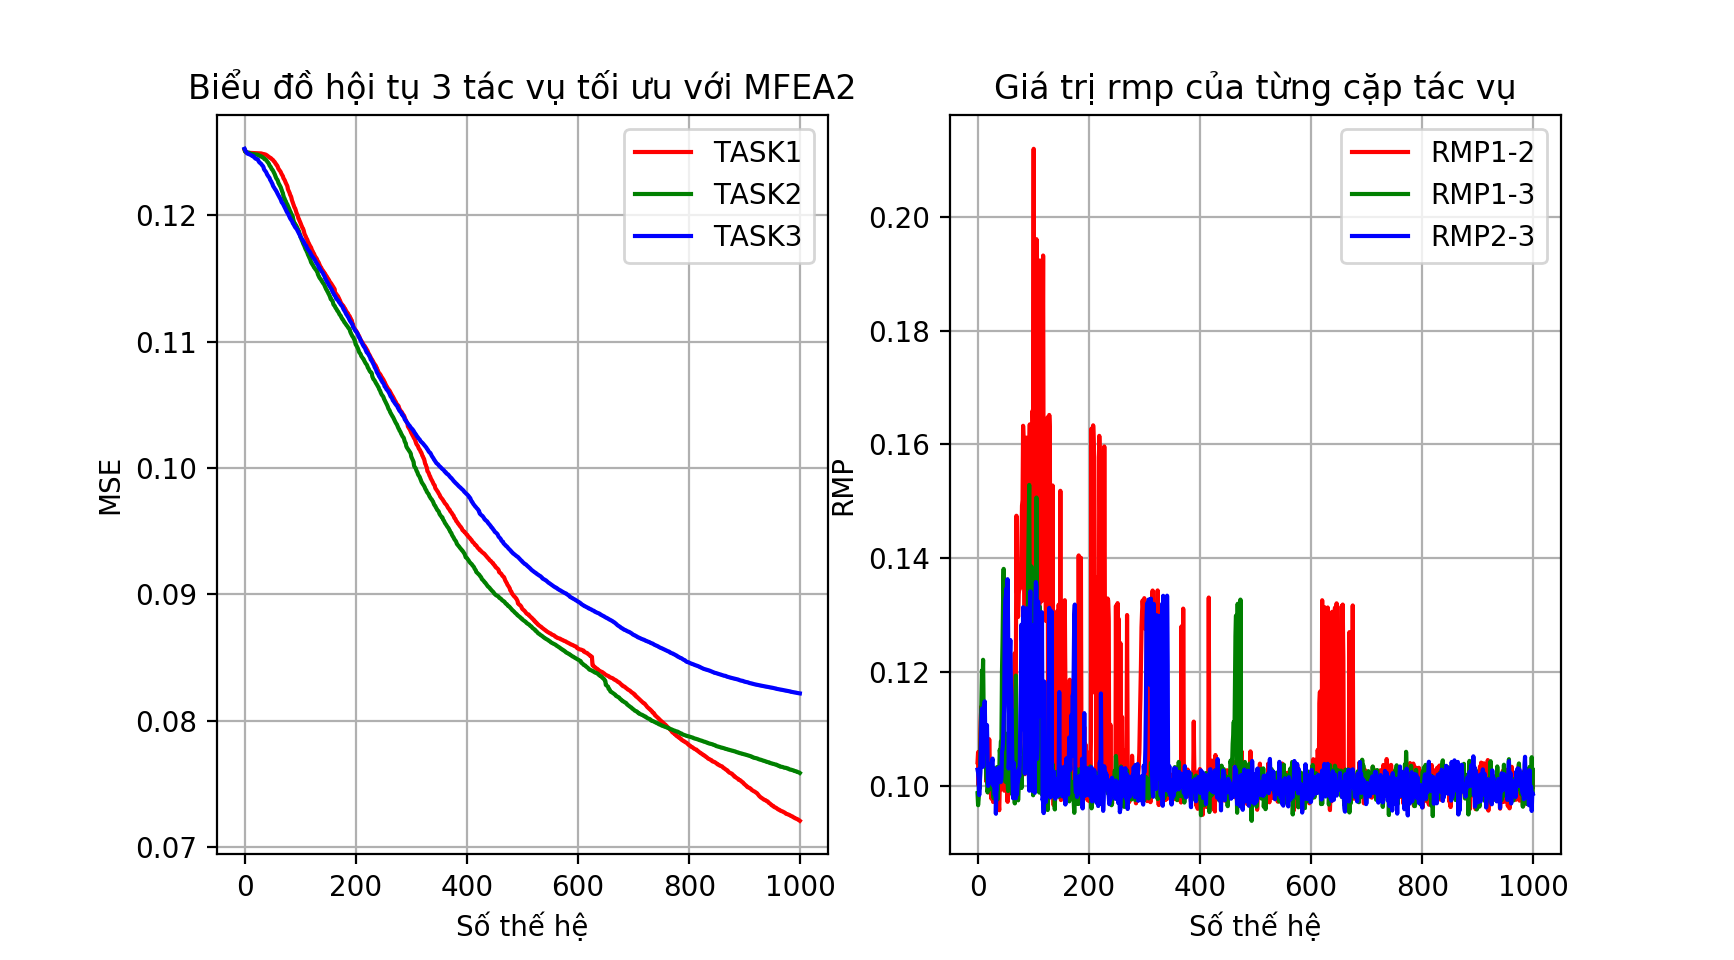
\includegraphics[width=\textwidth,height=\textheight,keepaspectratio]{thesis/images/results/multilayers/8bit2_rmp.png}}
    \caption{Bài 8bit: Biểu đồ hội tụ của từng tác vụ trên các thuật toán và biểu đồ phân tích MFEA-II theo giá trị rmp}
    \label{fig:8bit_multilayer}
\end{figure}
\begin{figure}[h!]
    \centering
    \scalebox{.6}{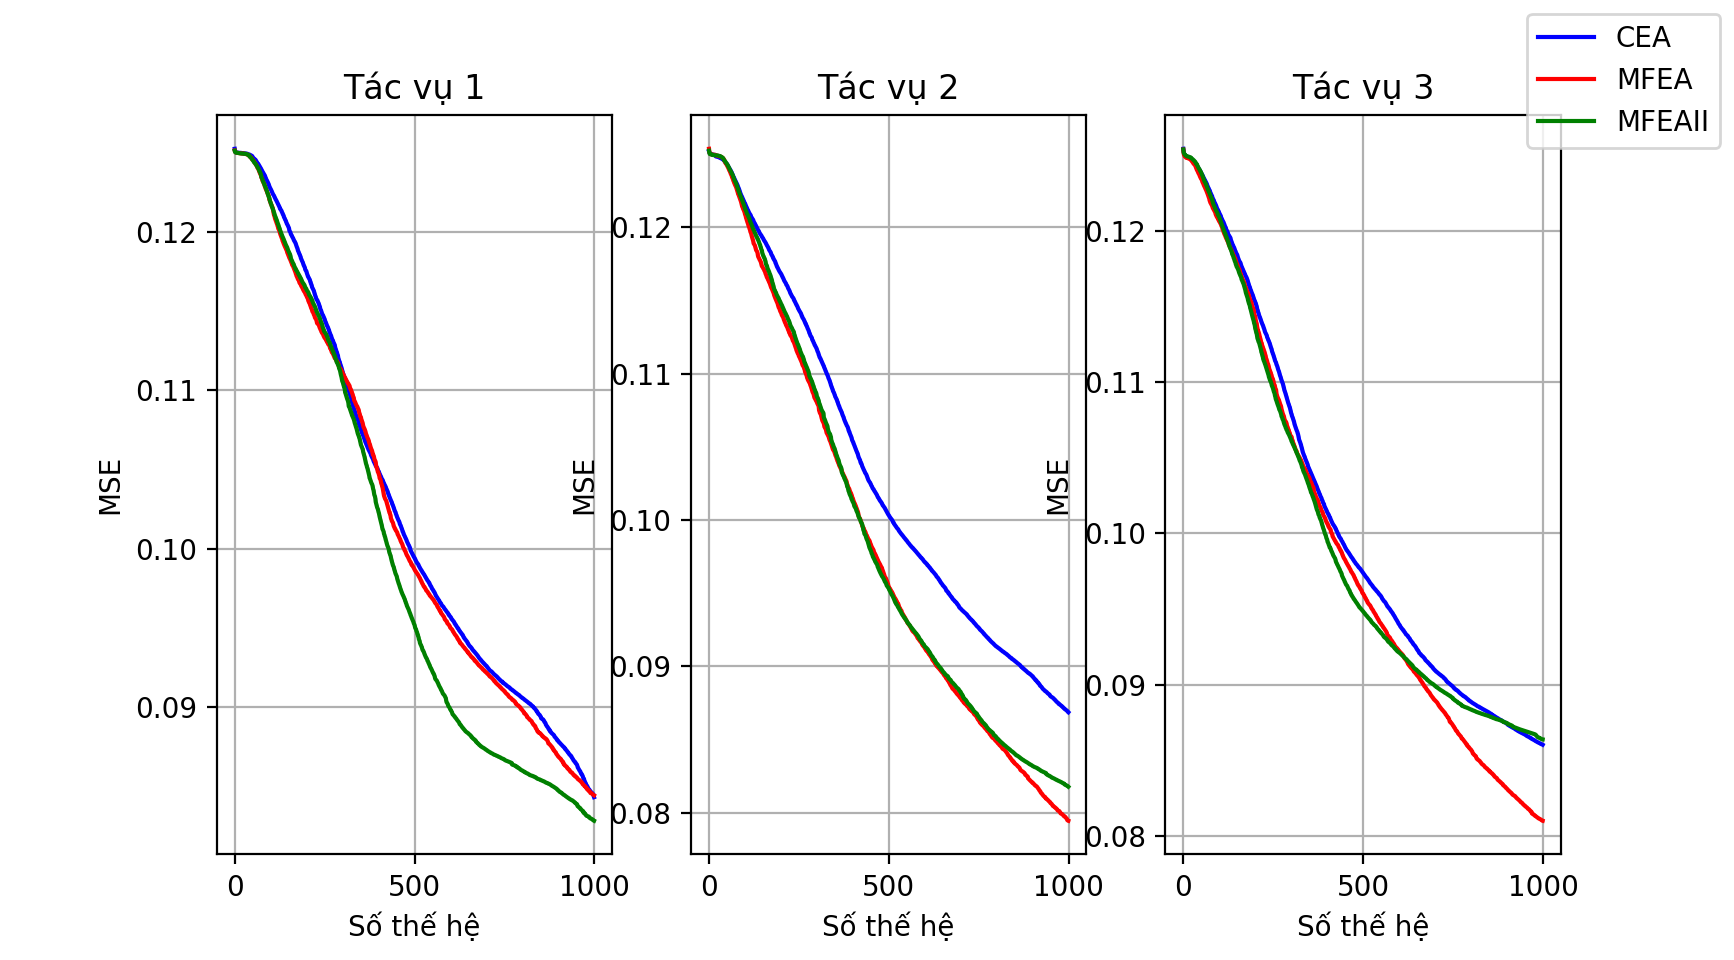
\includegraphics[width=\textwidth,height=\textheight,keepaspectratio]{thesis/images/results/multilayers/9bit2_task.png}}
    \scalebox{.6}{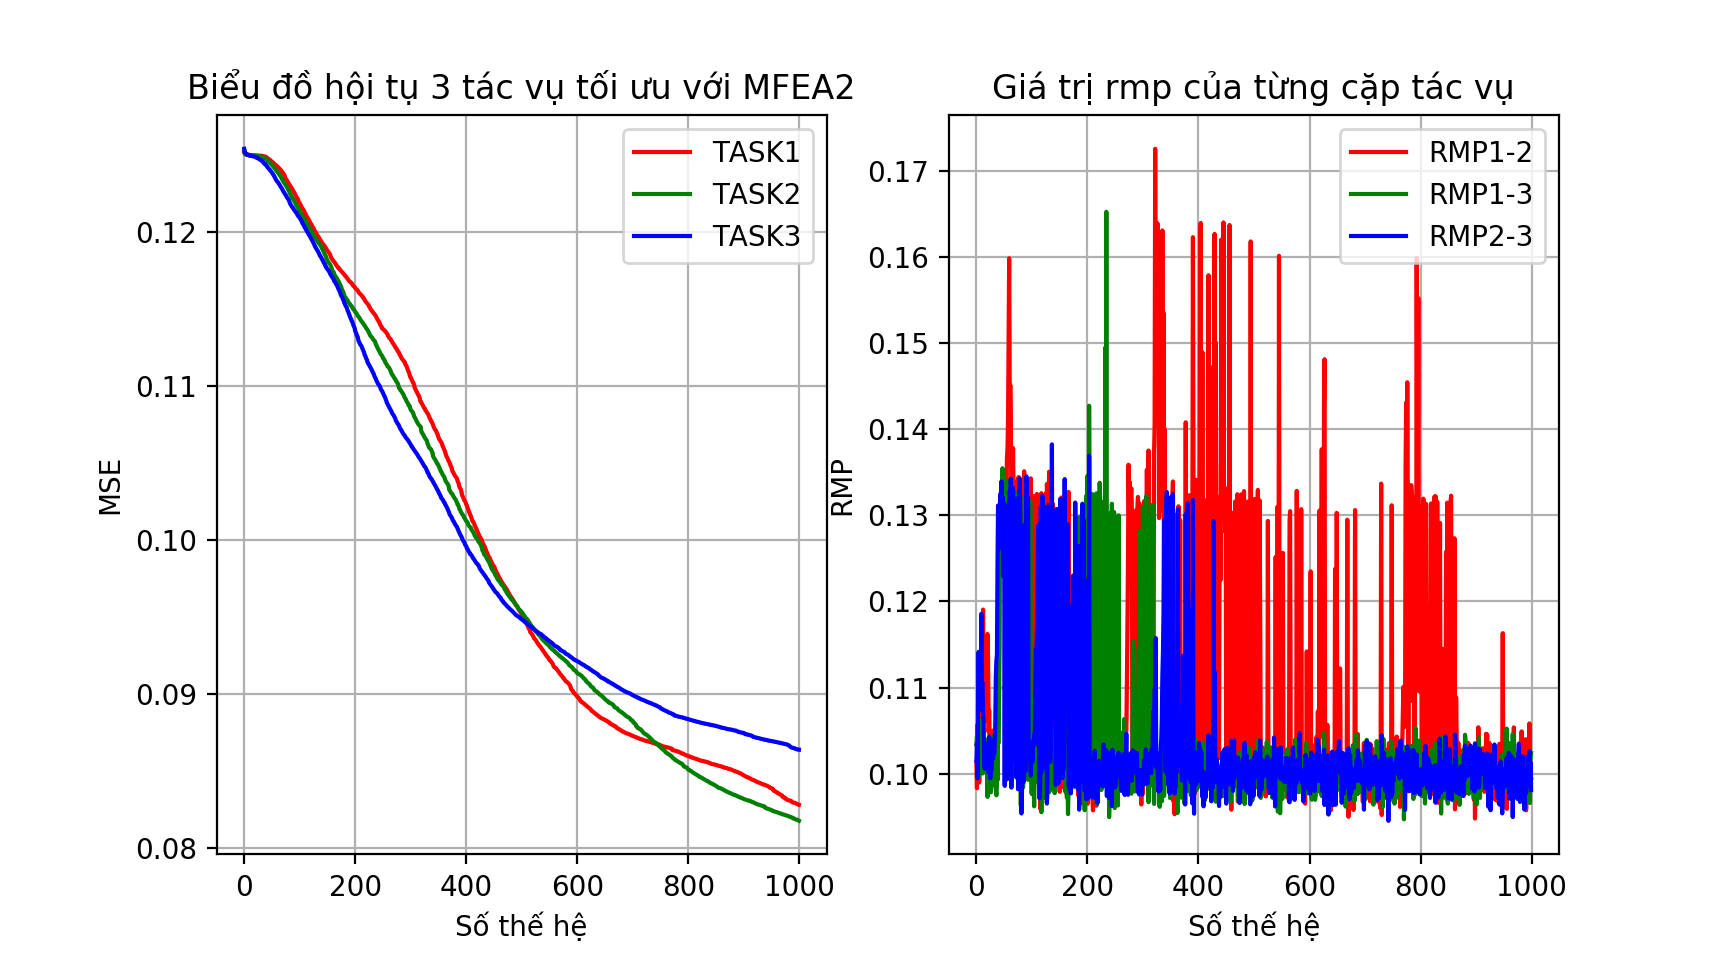
\includegraphics[width=\textwidth,height=\textheight,keepaspectratio]{thesis/images/results/multilayers/9bit2_rmp.png}}
    \caption{Bài 9bit: Biểu đồ hội tụ của từng tác vụ trên các thuật toán và biểu đồ phân tích MFEA-II theo giá trị rmp}
    \label{fig:8bit_multilayer}
\end{figure}
\begin{figure}[h!]
    \centering
    \scalebox{.5}{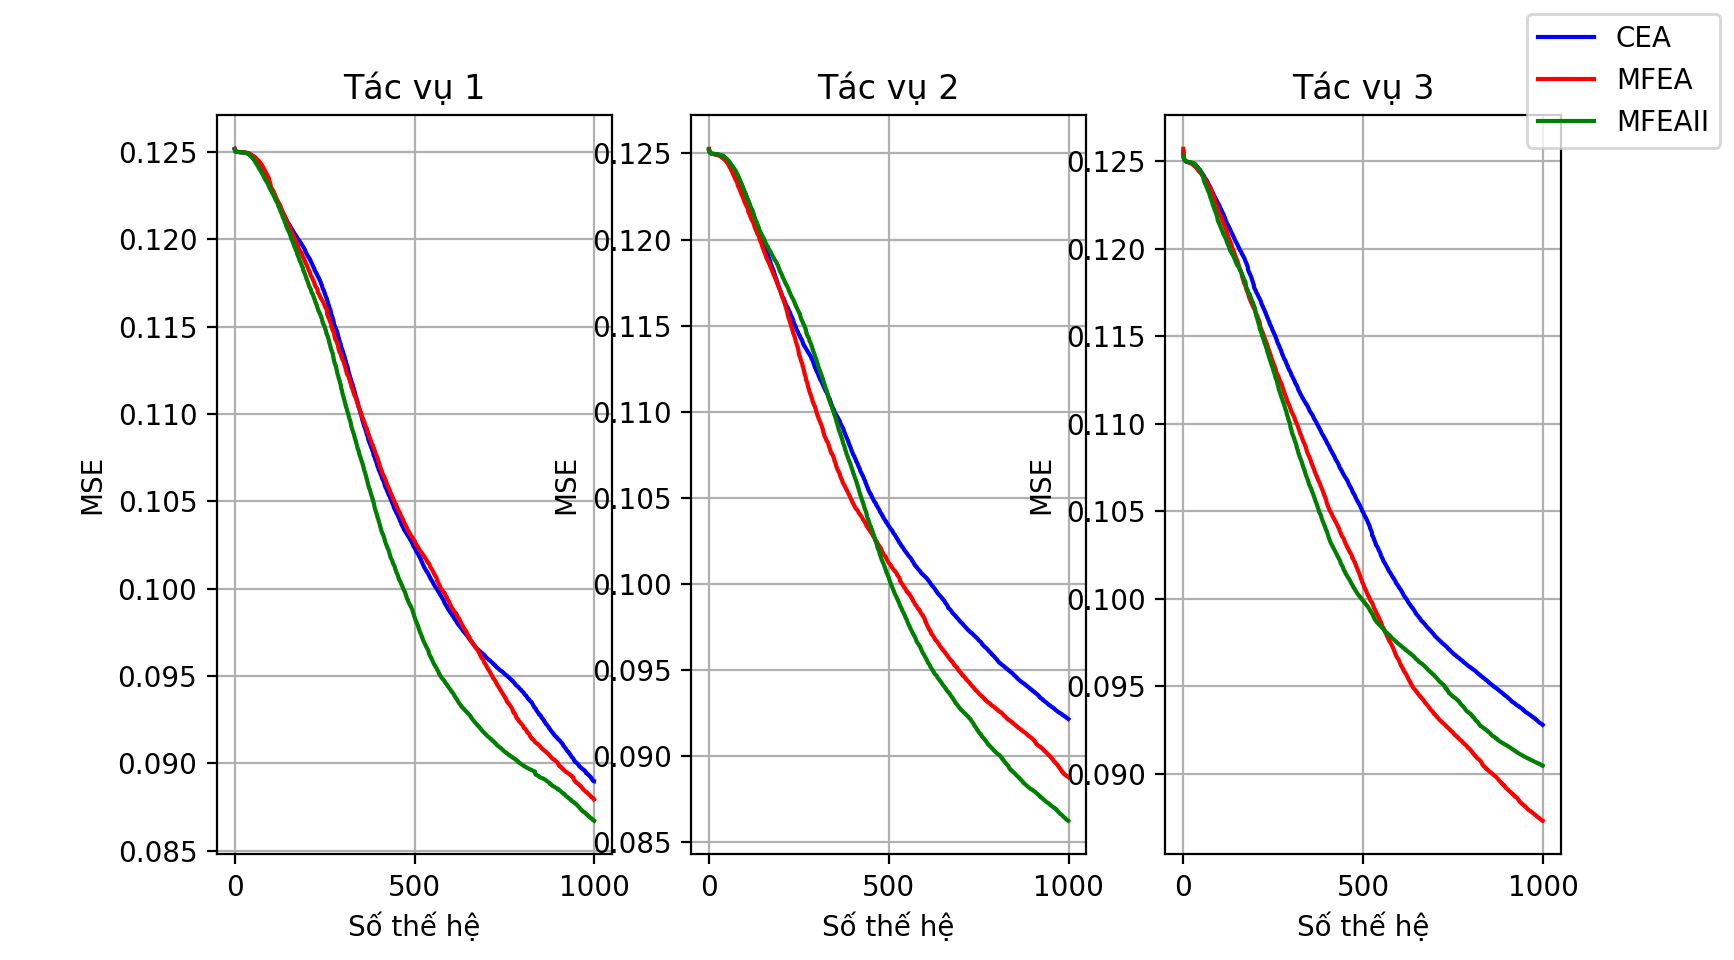
\includegraphics[width=\textwidth,height=\textheight,keepaspectratio]{thesis/images/results/multilayers/10bit2_task.png}}
    \scalebox{.5}{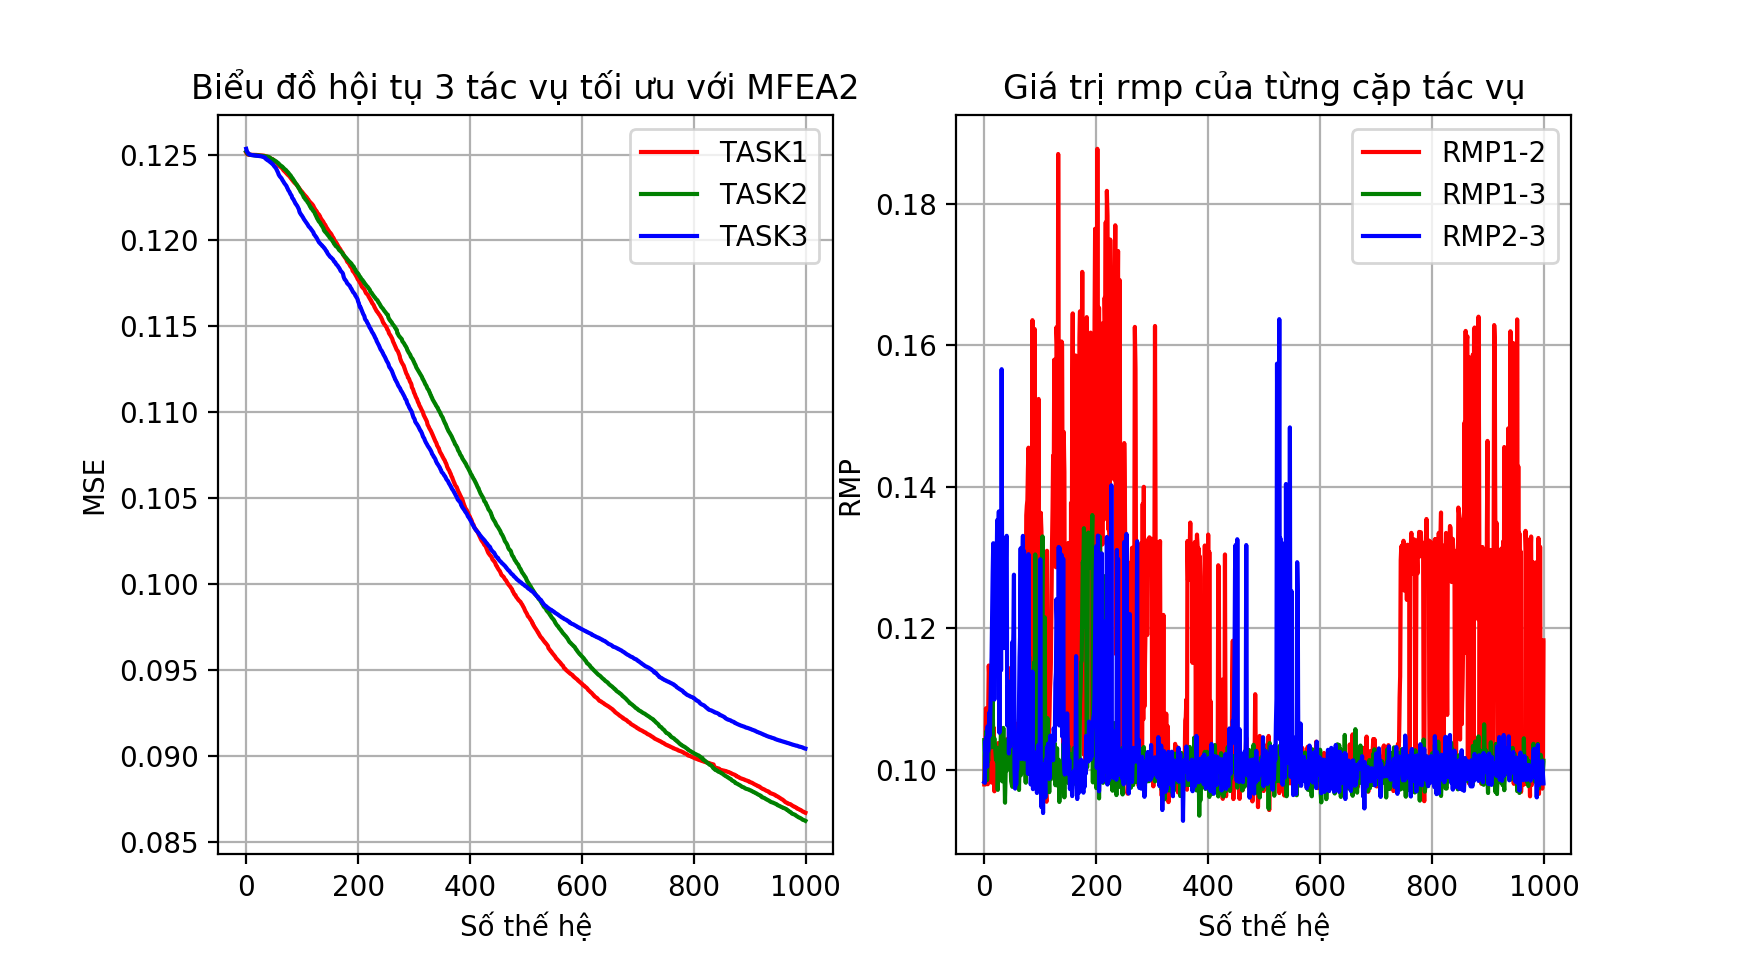
\includegraphics[width=\textwidth,height=\textheight,keepaspectratio]{thesis/images/results/multilayers/10bit2_rmp.png}}
    \caption{Bài 10bit: Biểu đồ hội tụ của từng tác vụ trên các thuật toán và biểu đồ phân tích MFEA-II theo giá trị rmp}
    \label{fig:8bit_multilayer}
\end{figure}

\subsubsection{Bảng kết quả thực nghiệm - bộ dữ liệu UCI với mạng neural cùng độ sâu}
\begin{table}[h!]
    \caption{Kết quả huấn luyện nhiều ANN trên bộ dữ liệu UCI cùng độ sâu}

    \begin{tabular}{|c|c|c|c|c|}
    \hline
    \multirow{1}{*}{\textbf{Instance}} & \multicolumn{1}{c|} {\textbf{Method}} & \multicolumn{1}{c|}{\textbf{Subtask1}} & \multicolumn{1}{c|}{\textbf{Subtask 2}} & \multicolumn{1}{c|}{\textbf{Subtask 3}} \\ \hline
    \multirow{3}{*} 
    {breastCancer} & CEA & $0.0097 \pm 0.0012$ & $0.0092 \pm 0.0007$ & $0.0093 \pm 0.0009$ \\
     & MFEA-I & $0.0097 \pm 0.0006$ & $0.0093 \pm 0.0005$ & $0.0091 \pm 0.0005$ \\ 
    & MFEA II & $\mathbf{0.0094 \pm 0.0008}$ & $\mathbf{0.0089 \pm 0.0006}$ & $\mathbf{0.0087 \pm 0.0004}$ \\ \hline
    \multirow{3}{*} {creditScreening} & CEA & $0.0509 \pm 0.0033$ & $0.0514 \pm 0.0033$ & $0.0508 \pm 0.004$ \\
   & MFEA-I & $0.0504 \pm 0.0024$ & $0.0503 \pm 0.0025$ & $0.0513 \pm 0.0022$ \\ 
   & MFEA-II & $\mathbf{0.0492 \pm 0.0023}$ & $\mathbf{0.0489 \pm 0.002}$ & $\mathbf{0.0491 \pm 0.002}$ \\ \hline
    \multirow{3}{*} {ionosphere} & CEA & $0.0384 \pm 0.0072$ & $0.0389 \pm 0.0129$ & $0.035 \pm 0.0047$ \\
    &MFEA-I & $0.0367 \pm 0.0068$ & $0.0347 \pm 0.0075$ & $0.0351 \pm 0.0088$ \\
    &MFEA-II & $\mathbf{0.0343 \pm 0.0079}$ & $\mathbf{0.0322 \pm 0.0071}$ & $\mathbf{0.032 \pm 0.007}$ \\\hline
    \multirow{3}{*} {ticTacToe} & CEA & $0.089 \pm 0.0047$ & $0.0838 \pm 0.0054$ & $0.0869 \pm 0.0049$ \\
    &MFEA-I & $0.0845 \pm 0.0049$ & $0.0818 \pm 0.0047$ & $0.0824 \pm 0.0047$ \\
    &MFEA-II & $\mathbf{0.082 \pm 0.0048}$ & $\mathbf{0.0815 \pm 0.0046}$ & $\mathbf{0.0812 \pm 0.0043}$  \\\hline
    
    \end{tabular}

    \label{tab:result:nbit}
\end{table}
\subsubsection{Biểu đồ hội tụ - bộ dữ liệu UCI với mạng neural cùng độ sâu}

\begin{figure}[h!]
    \centering
    \scalebox{.7}{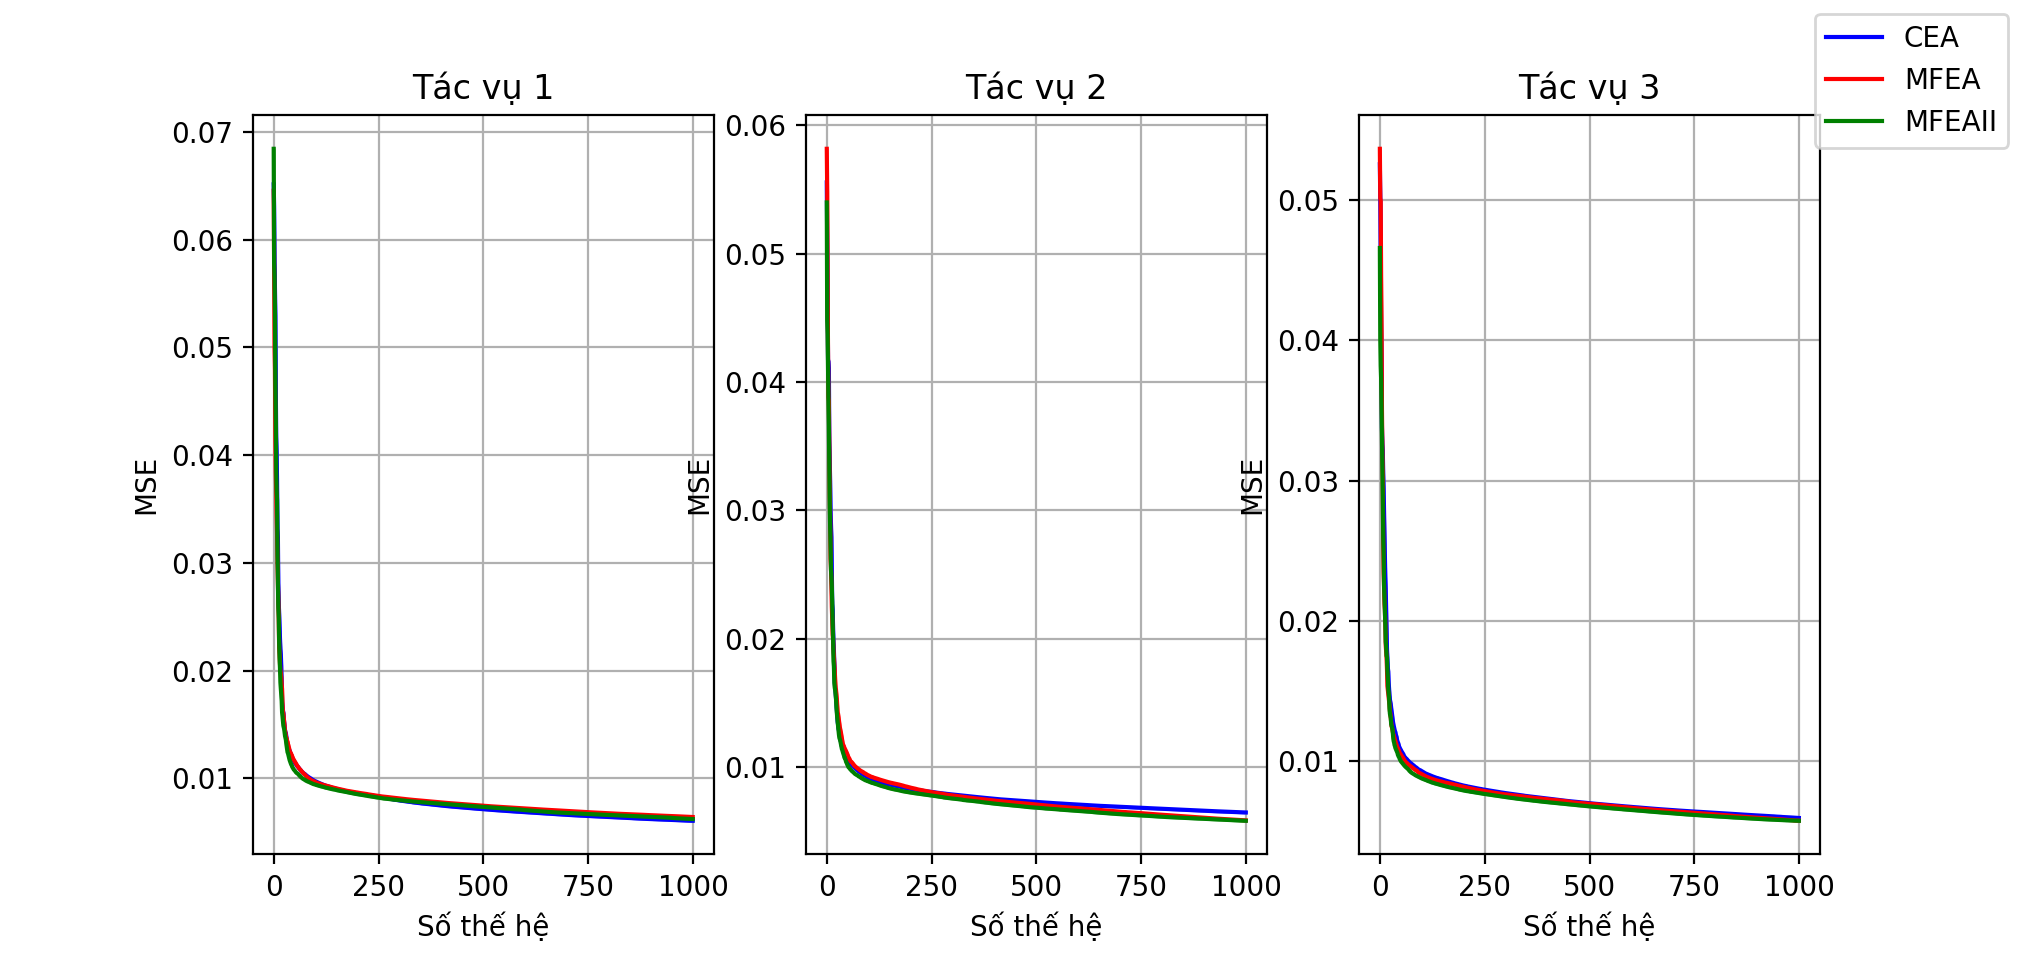
\includegraphics[width=\textwidth,height=\textheight,keepaspectratio]{thesis/images/results/uci/br1_task.png}}
    \scalebox{.7}{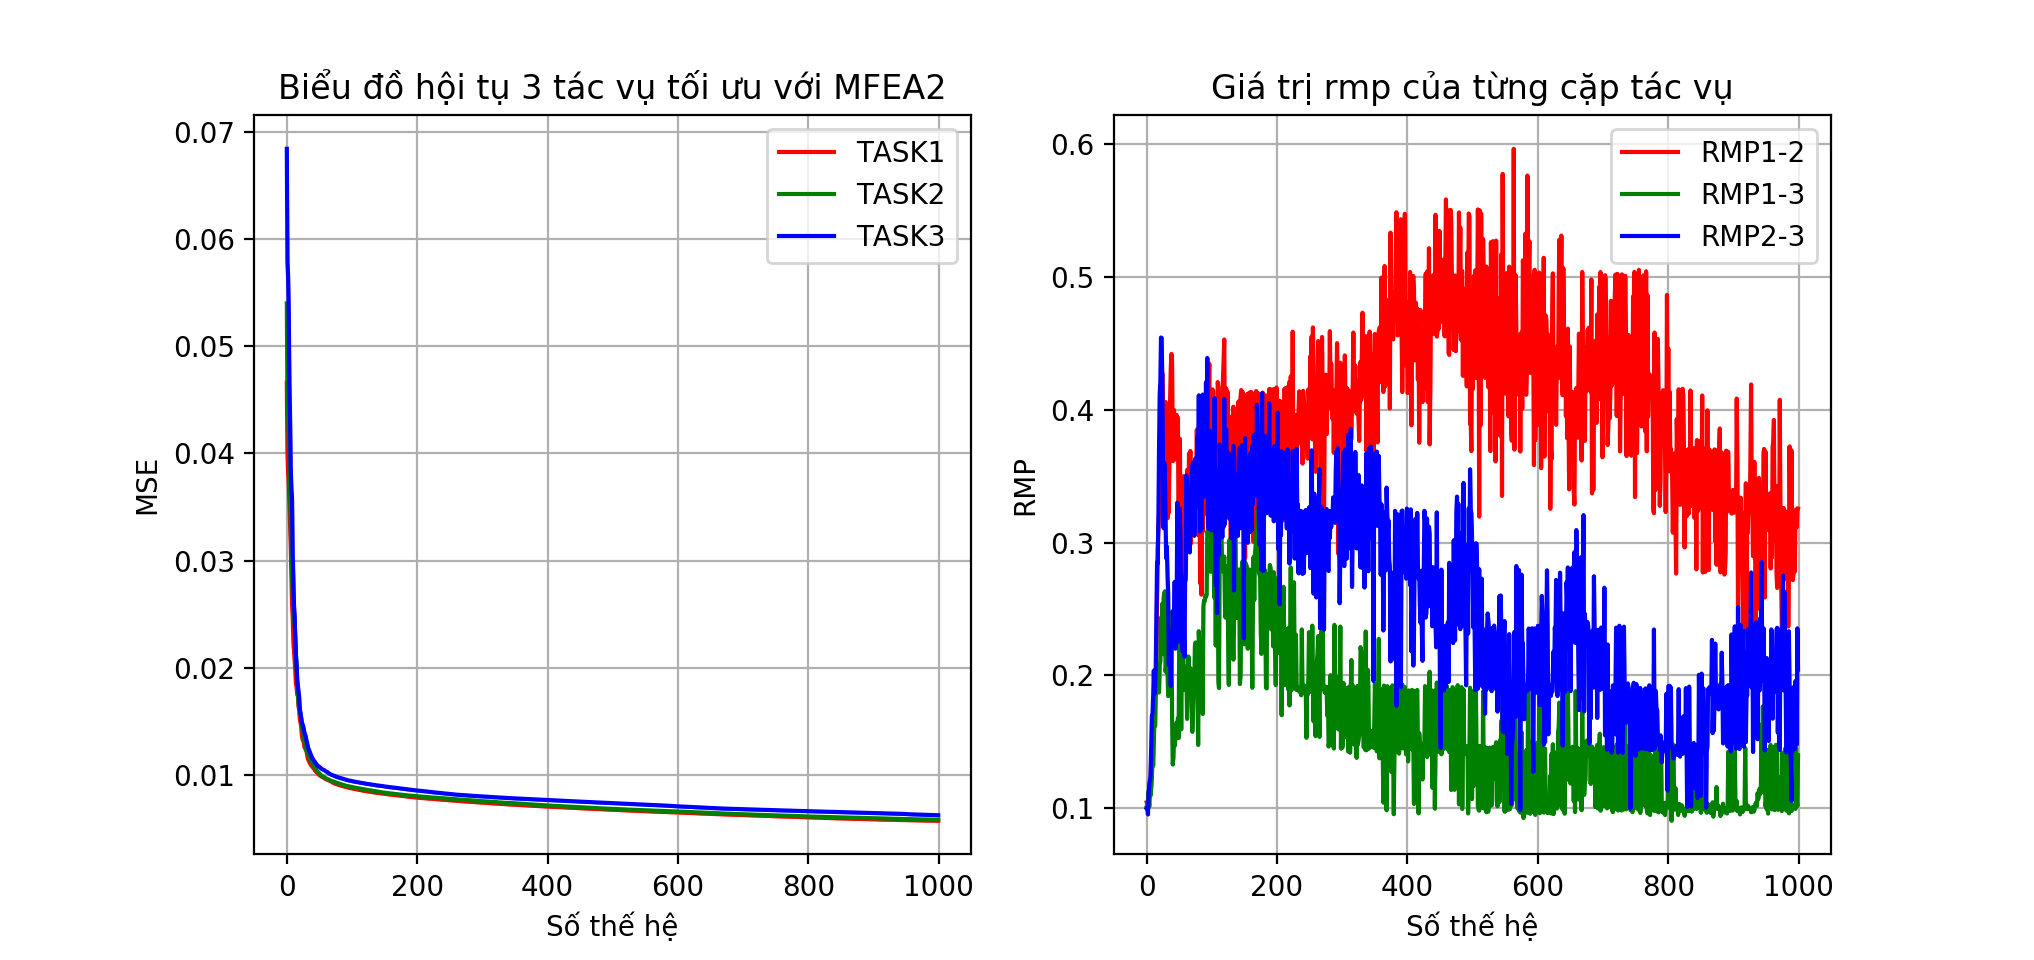
\includegraphics[width=\textwidth,height=\textheight,keepaspectratio]{thesis/images/results/uci/br1_rmp.png}}
    \caption{Biểu đồ hội tụ của các tác vụ bài BreastCancer cùng độ sâu}
    \label{fig:br_mtl}
\end{figure}

\begin{figure}[h!]
    \centering
    \scalebox{.7}{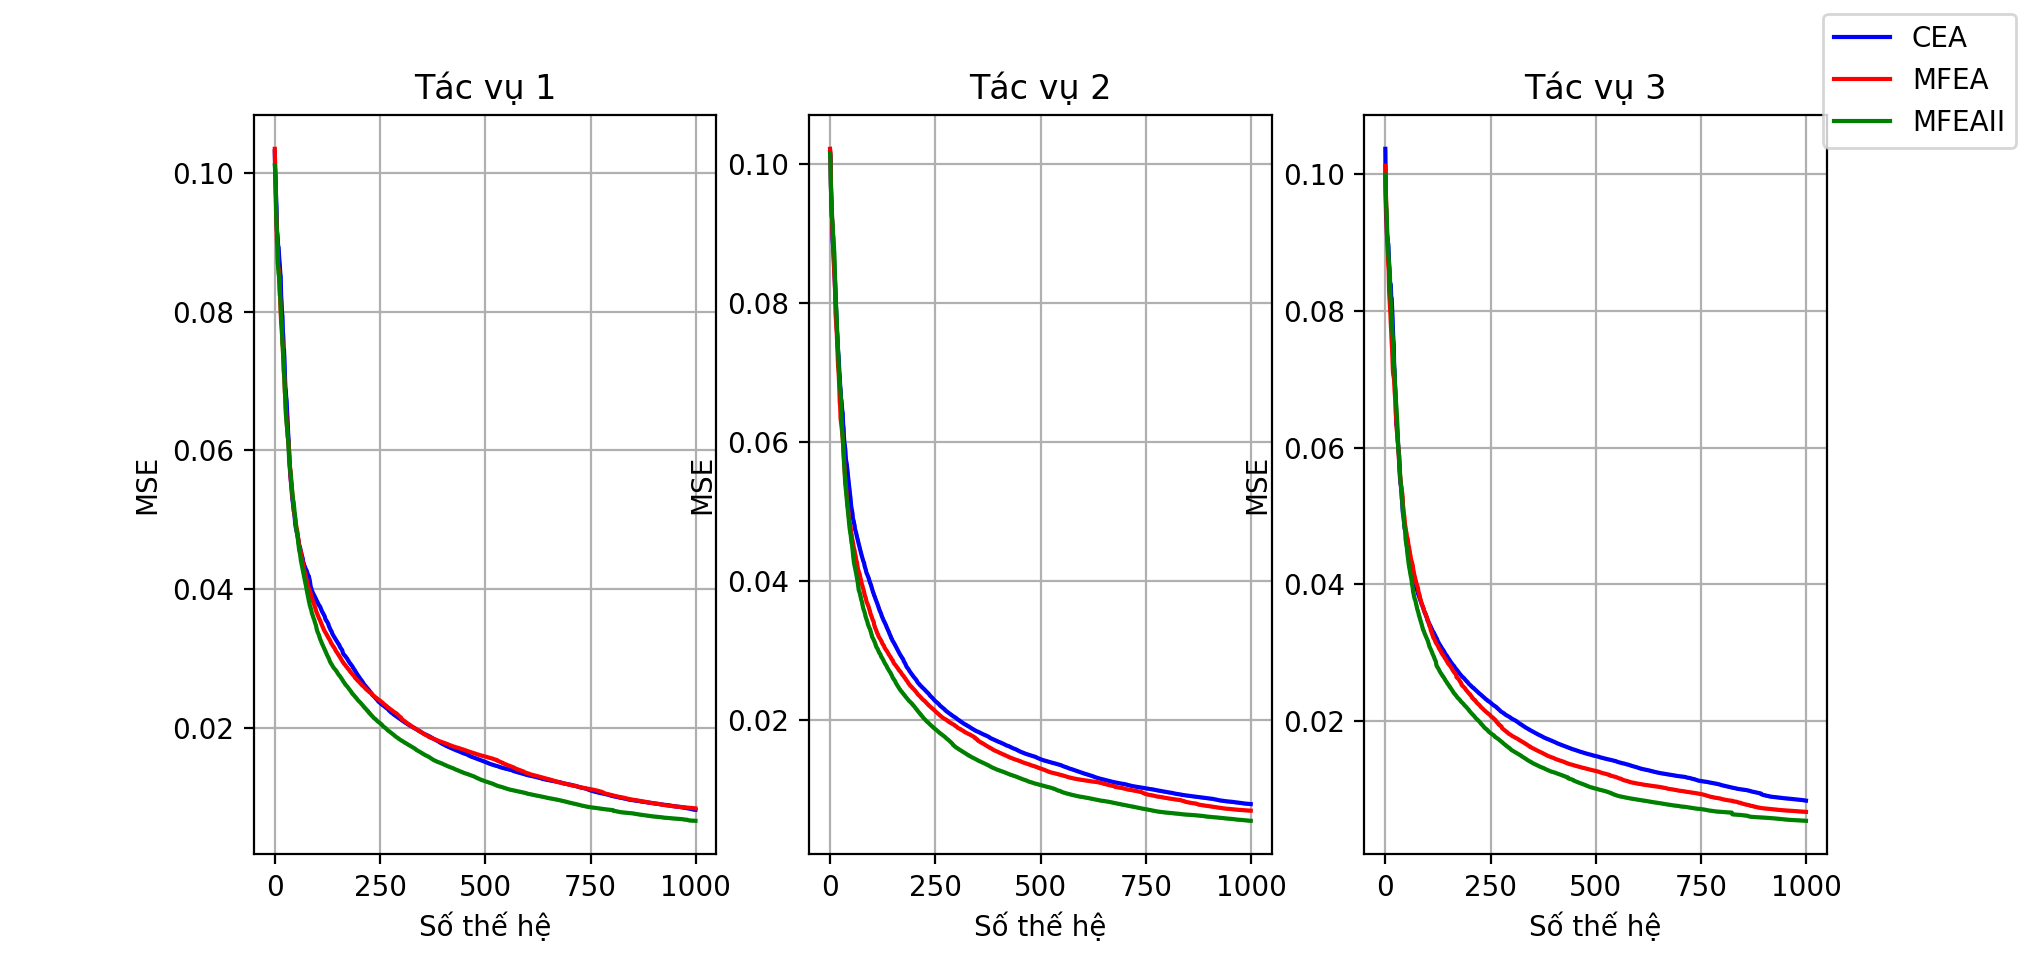
\includegraphics[width=\textwidth,height=\textheight,keepaspectratio]{thesis/images/results/uci/is1_task.png}}
    \scalebox{.7}{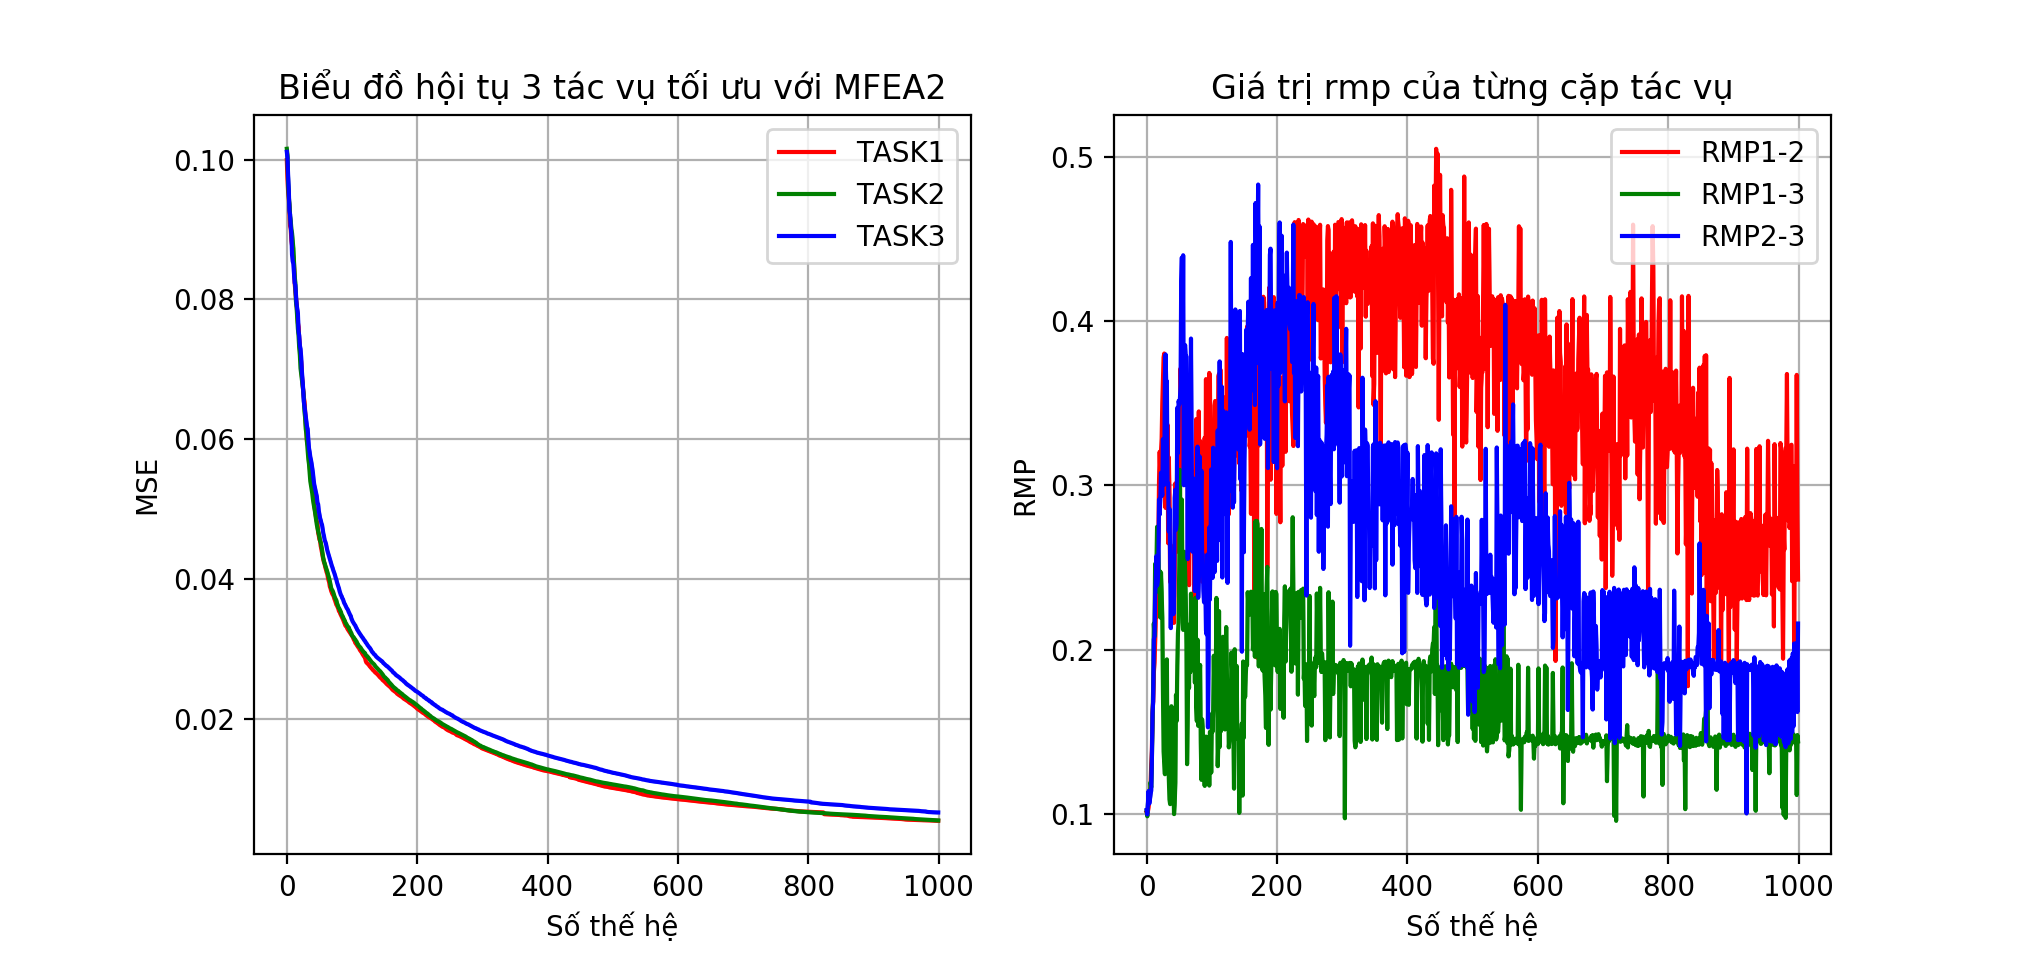
\includegraphics[width=\textwidth,height=\textheight,keepaspectratio]{thesis/images/results/uci/is1_rmp.png}}
    \caption{Biểu đồ hội tụ của các tác vụ bài Ionosphere cùng độ sâu}
    \label{fig:br_mtl}
\end{figure}
\newpage
\subsubsection{Bảng kết quả thực nghiệm - bộ dữ liệu UCI với mạng neural khác độ sâu}
% \begin{table}[h!]
%     \caption{Huấn luyện nhiều ANN trên bộ dữ liệu UCI khác độ sâu}
%     \begin{tabular}{|c|c|c|c|c|}
%     \hline
%     \multirow{1}{*}{\textbf{Instance}} & \multicolumn{1}{c|} {\textbf{Method}} & \multicolumn{1}{c|}{\textbf{Subtask1}} & \multicolumn{1}{c|}{\textbf{Subtask 2}} & \multicolumn{1}{c|}{\textbf{Subtask 3}} \\ \hline
%     \multirow{3}{*} 
%     {breastCancer} & CEA & $0.0119 \pm 0.0029$ & $0.0107 \pm 0.002$ & $\mathbf{0.0093 \pm 0.0005}$ \\
%      & MFEA-I & $\mathbf{0.011 \pm 0.0015}$ & $0.0102 \pm 0.0012$ & $0.0094 \pm 0.0005$  \\ 
%     & MFEA II & $\mathbf{0.011 \pm 0.0015}$ & $\mathbf{0.01 \pm 0.0011}$ & $0.0096 \pm 0.0011$ \\ \hline
    
%     \multirow{3}{*} {creditScreening} & CEA & $0.054 \pm 0.0071$ & $0.0503 \pm 0.0027$ & $0.0485 \pm 0.0017$ \\
%   & MFEA-I & $\mathbf{0.0508 \pm 0.0023}$ & $0.0497 \pm 0.0019$ & $0.0496 \pm 0.0021$ \\ 
%   & MFEA-II & $0.0515 \pm 0.0033$ & $\mathbf{0.0494 \pm 0.0023}$ & $\mathbf{0.0485 \pm 0.0018}$ \\ \hline
   
%     \multirow{3}{*} {ionosphere} & CEA & $0.0516 \pm 0.0124$ & $0.0449 \pm 0.0114$ & $0.0366 \pm 0.0094$ \\
%     &MFEA-I & $0.049 \pm 0.0131$ & $0.0413 \pm 0.0112$ & $\mathbf{0.0365 \pm 0.007}$ \\
%     &MFEA-II & $\mathbf{0.0473 \pm 0.0083}$ & $\mathbf{0.0387 \pm 0.0109}$ & $0.0367 \pm 0.008$  \\\hline
    
%     \multirow{3}{*} {ticTacToe} & CEA & $0.0899 \pm 0.0067$ & $0.0879 \pm 0.0079$ & $0.0852 \pm 0.0045$  \\
%     &MFEA-I & $\mathbf{0.088 \pm 0.008}$ & $0.0886 \pm 0.0064$ & $0.0843 \pm 0.0092$  \\
%     &MFEA-II & $\mathbf{0.088 \pm 0.0073}$ & $\mathbf{0.0832 \pm 0.0067}$ & $0\mathbf{.0817 \pm 0.0046}$  \\\hline
    
%     \end{tabular}

%     \label{tab:result:nbit}
% \end{table}
\begin{table}[h!]
    \caption{Kết quả huấn luyện nhiều ANN trên bộ dữ liệu UCI khác độ sâu}
    \begin{tabular}{|c|c|c|c|c|}
    \hline
    \multirow{1}{*}{\textbf{Instance}} & \multicolumn{1}{c|} {\textbf{Method}} & \multicolumn{1}{c|}{\textbf{Subtask1}} & \multicolumn{1}{c|}{\textbf{Subtask 2}} & \multicolumn{1}{c|}{\textbf{Subtask 3}} \\ \hline
    \multirow{3}{*} 
    {breastCancer} & CEA & $0.0082 \pm 0.0006$ & $0.0083 \pm 0.0006$ & $0.008 \pm 0.0004$ \\
     & MFEA-I & $0.0084 \pm 0.0007$ & $0.0081 \pm 0.0006$ & $0.008 \pm 0.0004$  \\ 
    & MFEA II & $\mathbf{0.0082 \pm 0.0006}$ & $\mathbf{0.008 \pm 0.0004}$ & $\mathbf{0.008 \pm 0.0004}$ \\ \hline
    
    \multirow{3}{*} {creditScreening} & CEA & $0.0442 \pm 0.0016$ & $0.0436 \pm 0.0011$ & $0.0435 \pm 0.0011$ \\
   & MFEA-I & $0.0446 \pm 0.0017$ & $\mathbf{0.0435 \pm 0.0012}$ & $0.0438 \pm 0.0013$ \\ 
   & MFEA-II & $\mathbf{0.0442 \pm 0.0016}$ & $0.0437 \pm 0.0014$ & $\mathbf{0.0433 \pm 0.0012}$ \\ \hline
   
    \multirow{3}{*} {ionosphere} & CEA & $\mathbf{0.0223 \pm 0.0064}$ & $\mathbf{0.0189 \pm 0.005}$ & $\mathbf{0.018 \pm 0.0063}$ \\
    &MFEA-I & $0.0257 \pm 0.01$ & $0.0213 \pm 0.0082$ & $0.0201 \pm 0.0076$ \\
    &MFEA-II & $0.0243 \pm 0.0055$ & $0.0199 \pm 0.0055$ & $0.0203 \pm 0.0062$  \\\hline
    
    \multirow{3}{*} {ticTacToe} & CEA & $0.0747 \pm 0.0077$ & $0.0728 \pm 0.0093$ & $0.0731 \pm 0.0061$   \\
    &MFEA-I & $0.0736 \pm 0.0103$ & $0.0724 \pm 0.008$ & $0.0704 \pm 0.0067$   \\
    &MFEA-II & $\mathbf{0.0709 \pm 0.0096}$ & $\mathbf{0.0667 \pm 0.0066}$ & $\mathbf{0.0684 \pm 0.0067}$  \\\hline
    
    \end{tabular}

    \label{tab:result:nbit}
\end{table}

\newpage
\subsubsection{Biểu đồ hội tụ - bộ dữ liệu UCI với mạng neural cùng độ sâu}

\begin{figure}[h!]
    \centering
    \scalebox{.7}{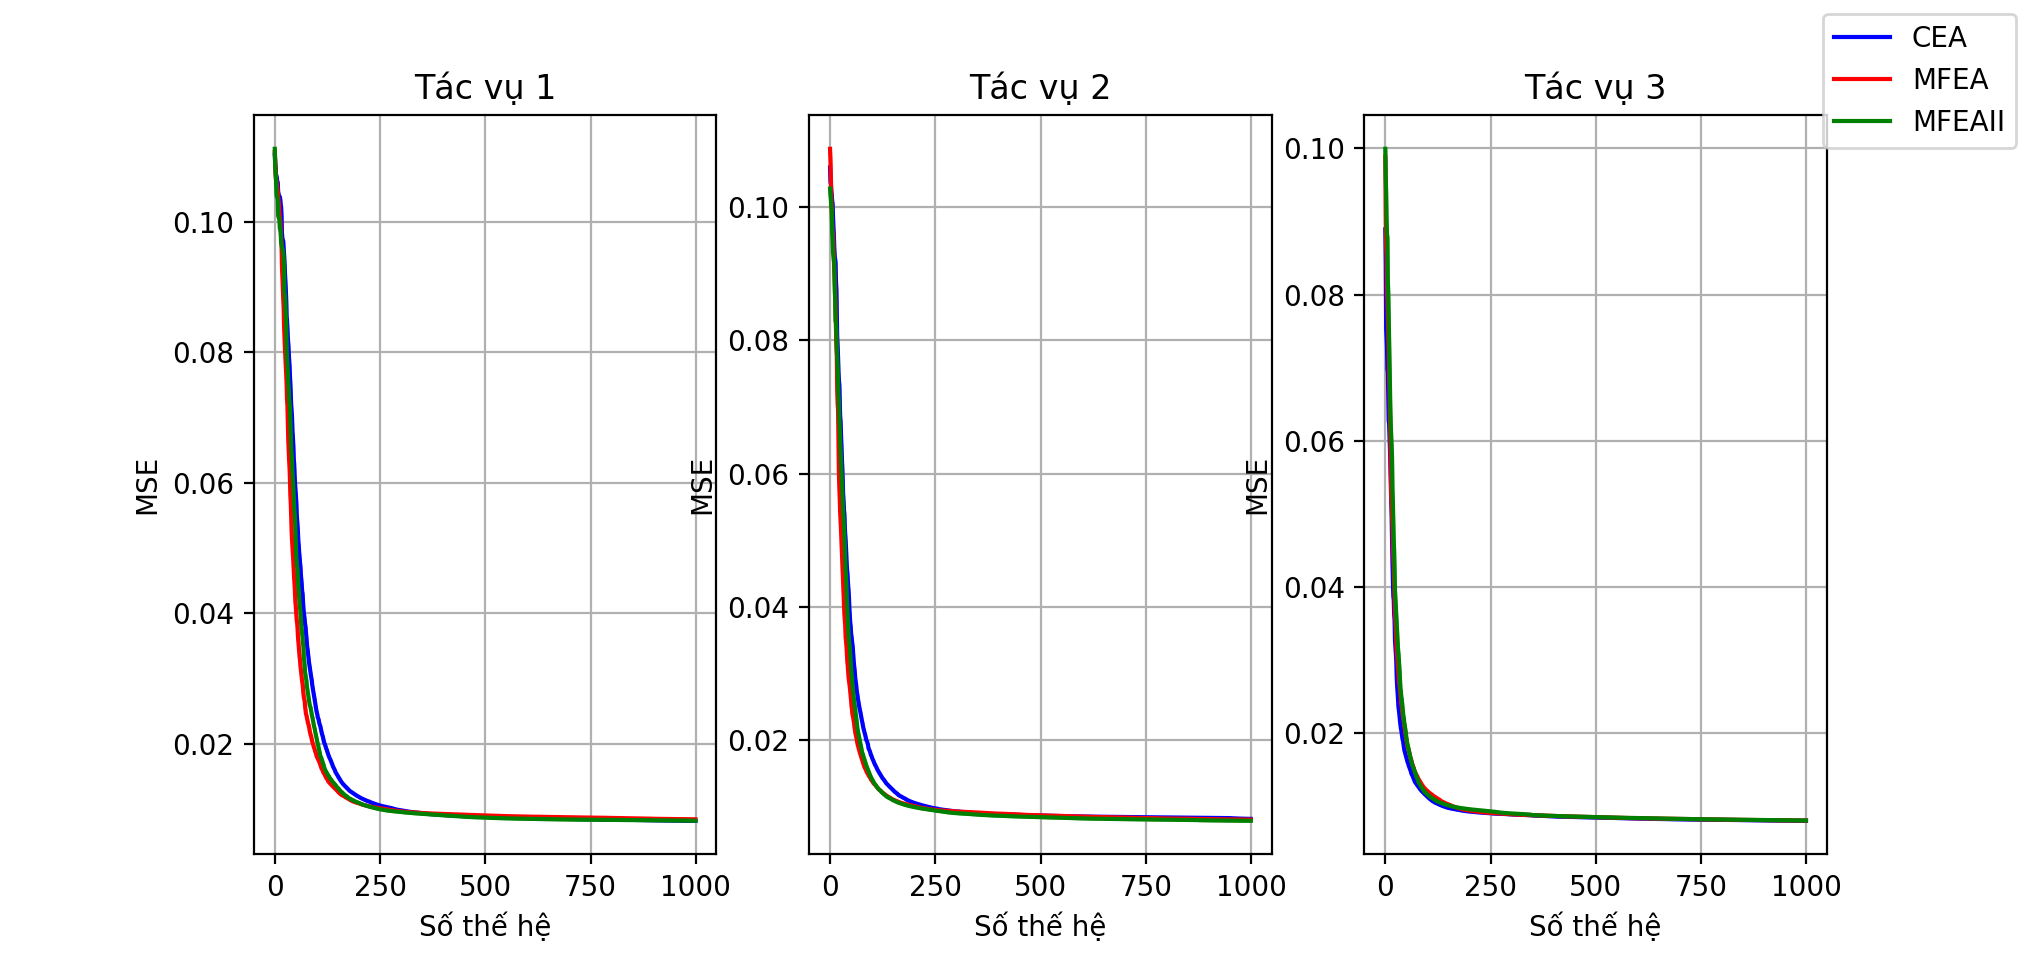
\includegraphics[width=\textwidth,height=\textheight,keepaspectratio]{thesis/images/results/uci/br_task.png}}
    \scalebox{.7}{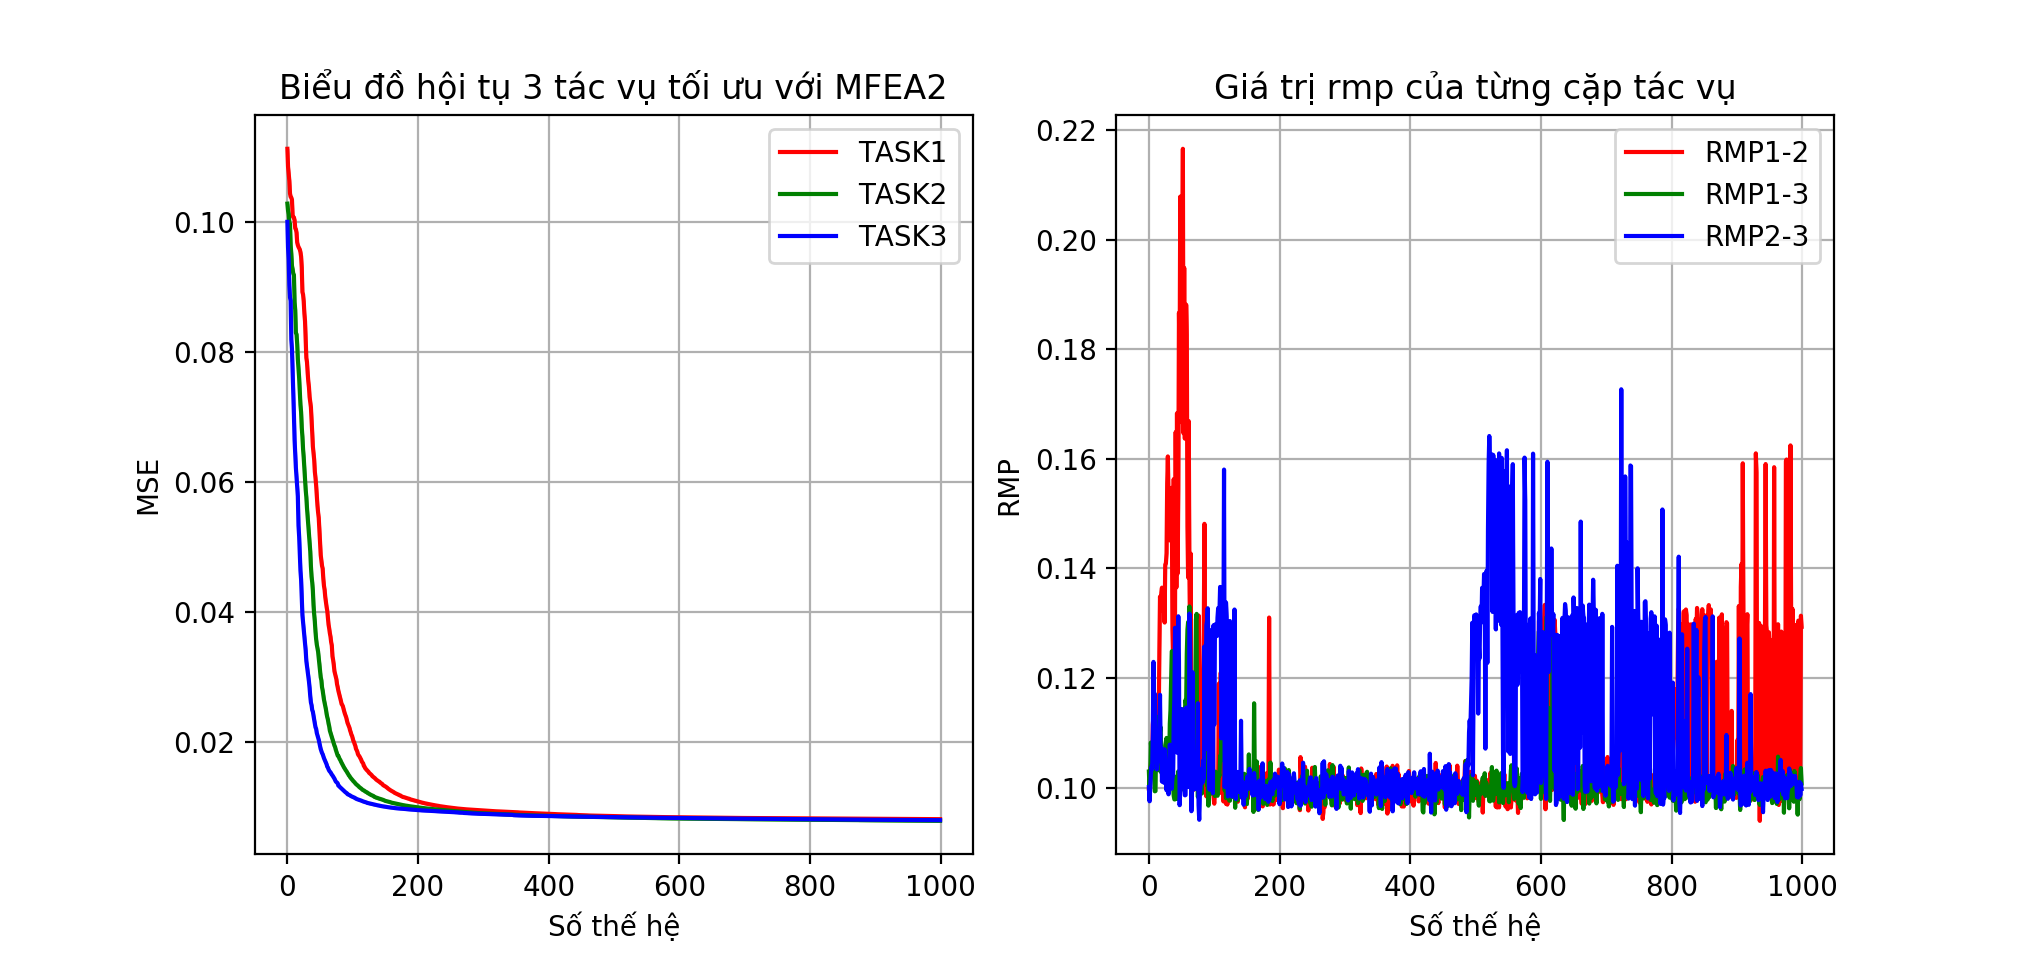
\includegraphics[width=\textwidth,height=\textheight,keepaspectratio]{thesis/images/results/uci/br_rmp.png}}
    \caption{Biểu đồ hội tụ bài BreastCancer khác độ sâu}
    \label{fig:br_mtl}
\end{figure}

\begin{figure}[h!]
    \centering
    \scalebox{.7}{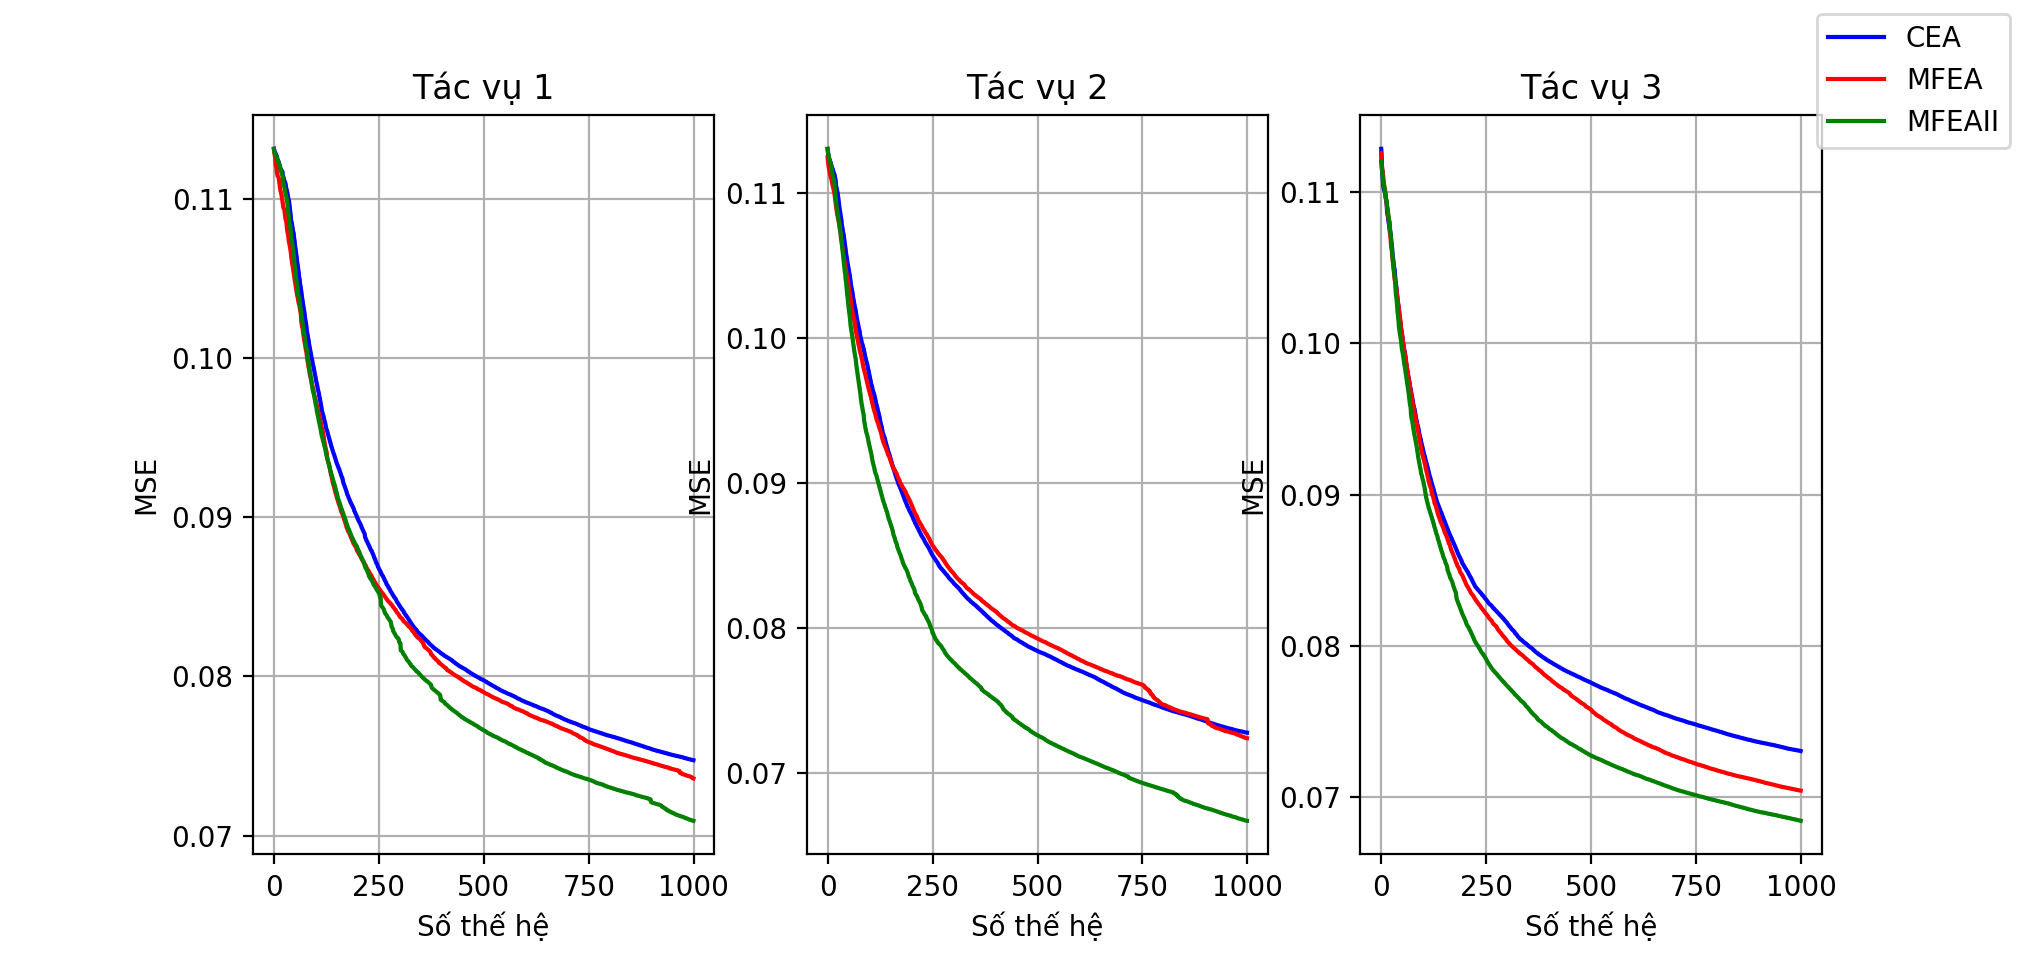
\includegraphics[width=\textwidth,height=\textheight,keepaspectratio]{thesis/images/results/uci/tt_task.png}}
    \scalebox{.7}{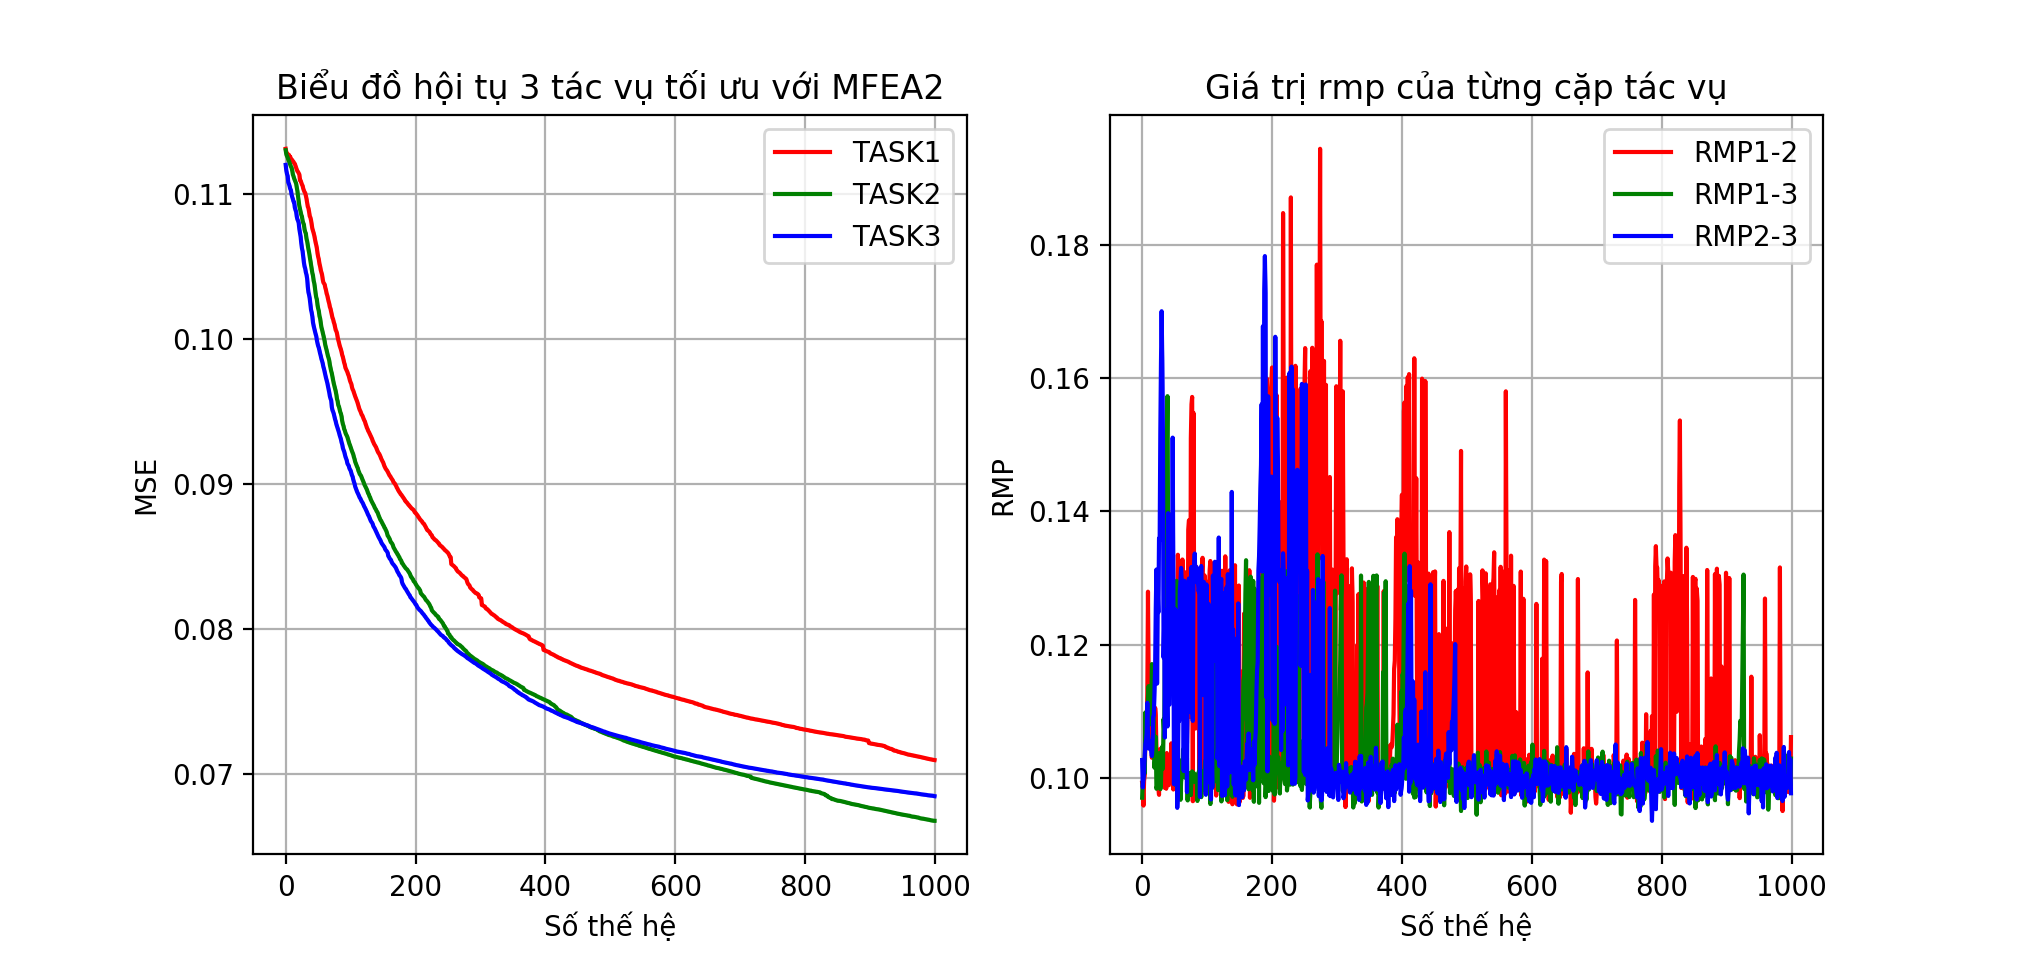
\includegraphics[width=\textwidth,height=\textheight,keepaspectratio]{thesis/images/results/uci/tt_rmp.png}}
    \caption{Biểu đồ hội tụ bài Tictactoe khác độ sâu}
    \label{fig:br_mtl}
\end{figure}
\pagebreak

\subsection{Kết quả huấn luyện trên các môi trường học tăng cường}
% \begin{table}
%     \caption{Mô hình học tăng cường khác môi trường}
%     \begin{center}
%     \begin{tabular}{|c|c|c|c|c|c|}
%     \hline
%     \multirow{1}{*}{\textbf{Trọng lực}} &
%     \multirow{1}{*}{\textbf{Method}} & \multicolumn{1}{c|}{\textbf{Cao nhất}} & {\textbf{Thấp nhất}} & \multicolumn{1}{c|}{\textbf{Trung Bình}} & \multicolumn{1}{c|}{\textbf{Độ lệch}} \\ \hline
%     \multirow{3}{*} 
%     {Trọng lực=1.0} &
%     CEA & $71$ & $4$ & $28.86$ & $17.16$ \\
%     & MFEAI & $\mathbf{129}$ & $17$ &$46.71$ & $20.36$  \\
%     & MFEAII & $84$ & $15$ & $\mathbf{52.81}$  &$15.45$\\\hline
%     \multirow{3}{*} 
%     {Trọng lực=1.98} &
%     CEA & $382$ & $7$ &$174.86$ & $113.79$ \\
%     & MFEAI  & $\mathbf{546}$ & $98$ & $\mathbf{319.86}$ & $95.34$ \\
%     & MFEAII & $517$ & $\mathbf{131}$ &$311.38$ & $106.76$ \\\hline
%     \multirow{3}{*} 
%     {Trọng lực=2.96} &
%     CEA & $272$ & $1$ &$97.9$ & $83.07$ \\
%     & MFEAI  & $\mathbf{349}$ & $\mathbf{140}$ & $\mathbf{222.81}$ & $52.07$ \\
%     & MFEAII & $322$ & $103$ &$212.38$ & $52.74$ \\\hline
%     \multirow{3}{*} 
%     {Trọng lực=3.94} &
%     CEA & $227$ & $2$ &$69.24$ & $56.64$ \\
%     & MFEAI  & $\mathbf{217}$ & $\mathbf{95}$ & $\mathbf{142.86}$ & $27.4$ \\
%     & MFEAII & $190$ & $76$ &$140.38$ & $27.78$ \\\hline
%     \multirow{3}{*} 
%     {Trọng lực=4.92} &
%     CEA & $95$ & $2$ & $25.48$ & $25.78$  \\
%     & MFEAI  & $\mathbf{181}$ & $\mathbf{54}$ & $90.86$ & $21.98$ \\
%     & MFEAII & $145$ & $44$ & $\mathbf{102.14}$ & $26.66$ \\\hline
%     \end{tabular}
%     \end{center}
    
%     \label{tab:result:nbit}
% \end{table}

\subsubsection{Bảng kết quả thực nghiệm - bài toán Acrobot}
\begin{table} [H]
    \begin{center}
    \caption{Kết quả huấn luyện các tác vụ cho bài toán Acrobot}

    \scalebox{0.9}{\begin{tabular}{|c|c|c|c|c|c|}
    \hline
    \multirow{1}{*}{\textbf{Thuật toán}} & \multicolumn{1}{c|}{\textbf{Tác vụ 1}} & \multicolumn{1}{c|}{\textbf{Tác vụ 2}} & \multicolumn{1}{c|}{\textbf{Tác vụ 3}} & \multicolumn{1}{c|}{\textbf{Tác vụ 4}} & \multicolumn{1}{c|}{\textbf{Tác vụ 5}} \\ \hline
    CEA & $-100 \pm 4.53$ & $-109.47 \pm 2.38$ & $-108.77 \pm 4.38$ & $-113.17 \pm 1.86$ & $-117.23 \pm 4.28$  \\
    MFEAI &  $-100 \pm 4.75$ & $\mathbf{-106.7 \pm 0.78}$ & $\mathbf{-108.3 \pm 4.47}$ & $-112.0 \pm 2.62$ & $-117.03 \pm 4.52$ \\
    MFEAII & $\mathbf{-100 \pm 4.7}$ & $-107.8 \pm 1.17$ & $-108.6 \pm 4.34$ & $\mathbf{-113.07 \pm 2.29}$ & $\mathbf{-116.9 \pm 4.09}$  \\\hline
    \end{tabular}}
    \end{center}
    \label{tab:result:acrobot}
\end{table}


\subsubsection{Biểu đồ hội tụ - bài toán Acrobot}
\begin{figure}[h!]
    \centering
    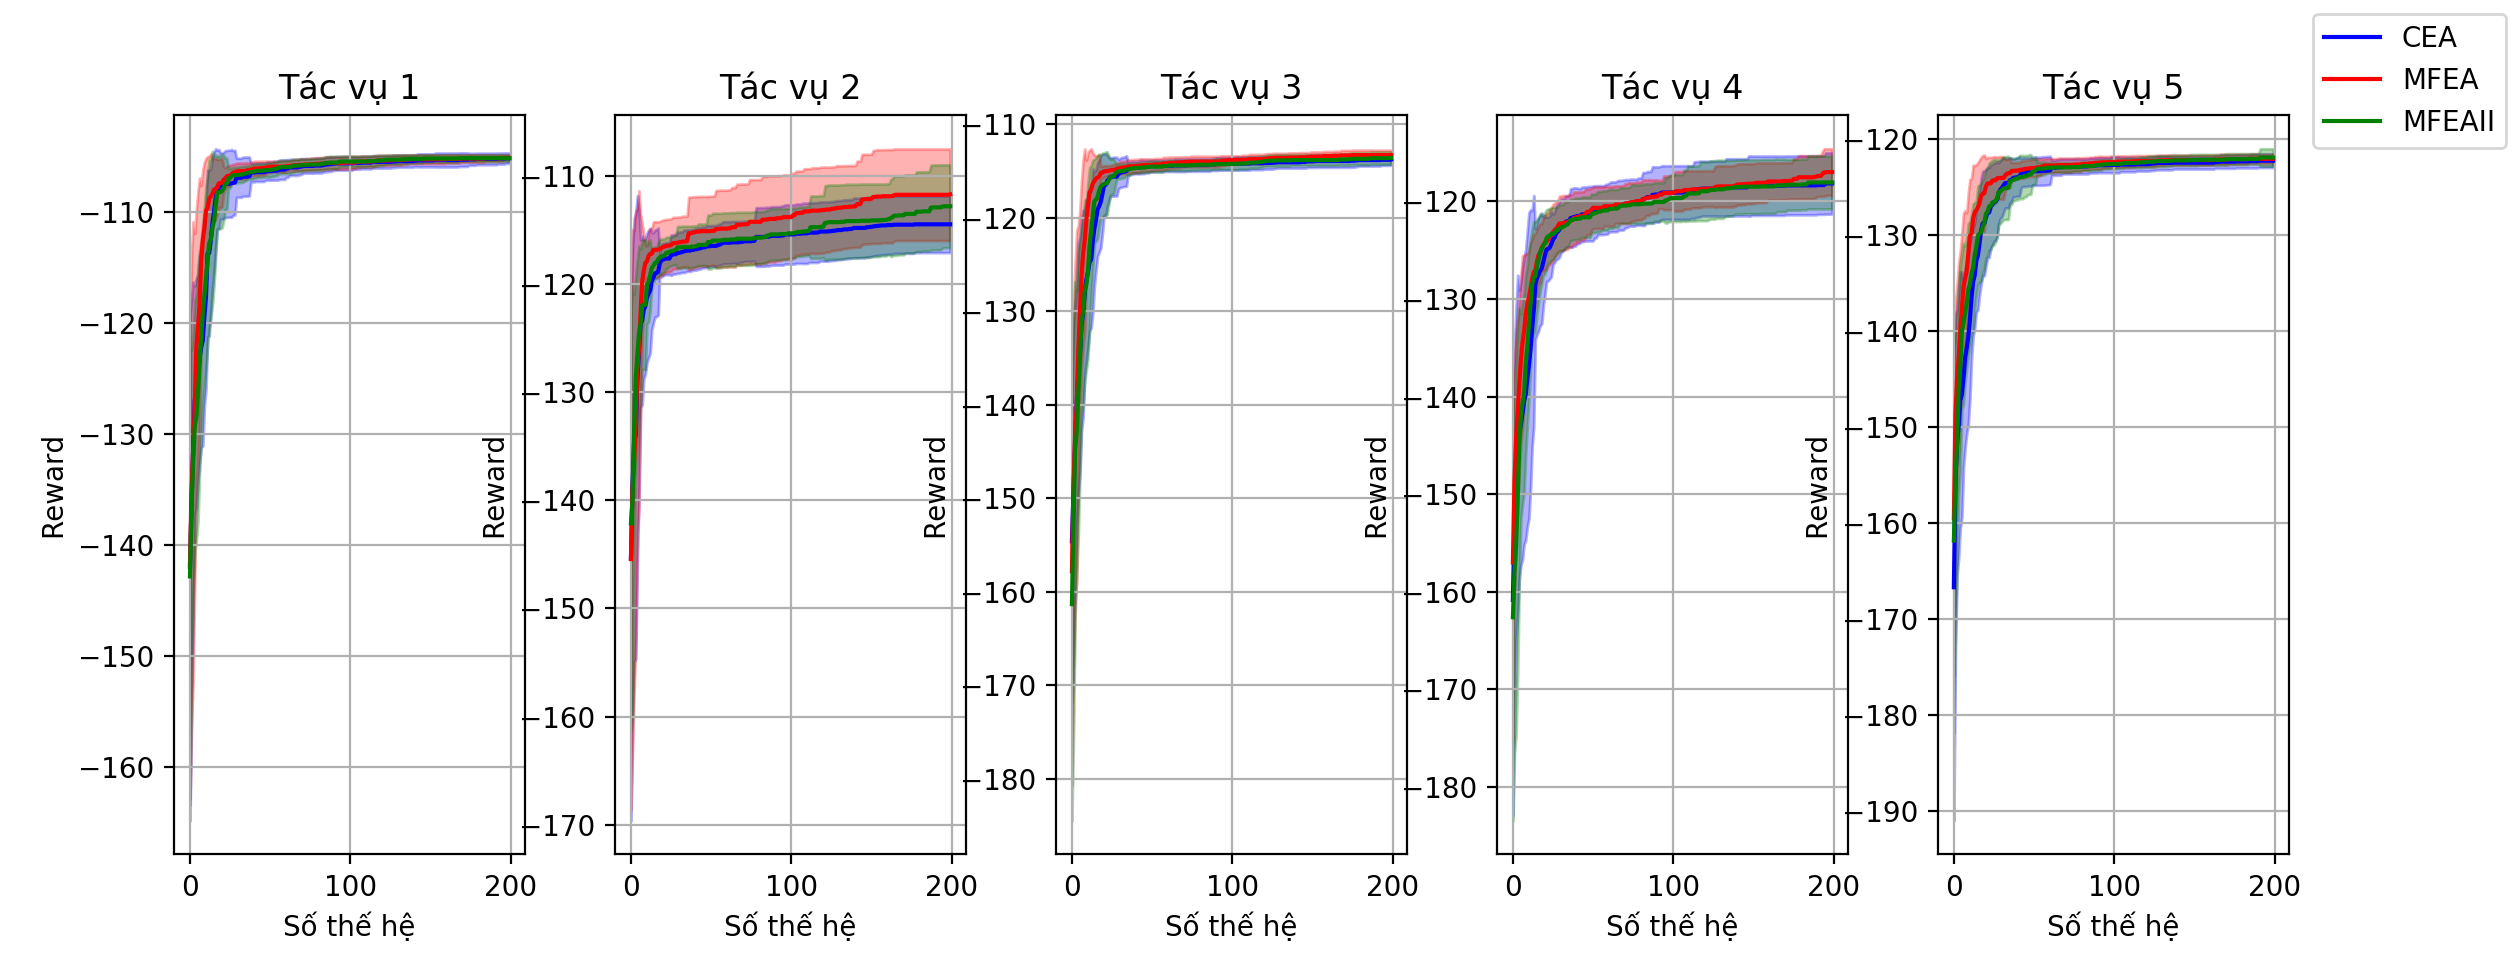
\includegraphics[width=\textwidth,height=\textheight,keepaspectratio]{thesis/images/results/rl/acrobot_conv.png}
    \caption{Biểu đồ hội tụ các tác vụ cho bài toán Acrobot}
    \label{fig:Acrobot_conv}
\end{figure}

\subsubsection{So sánh mức độ tập trung kết quả cuối cùng - bài toán Acrobot}
\begin{figure}[h!]
    \centering
    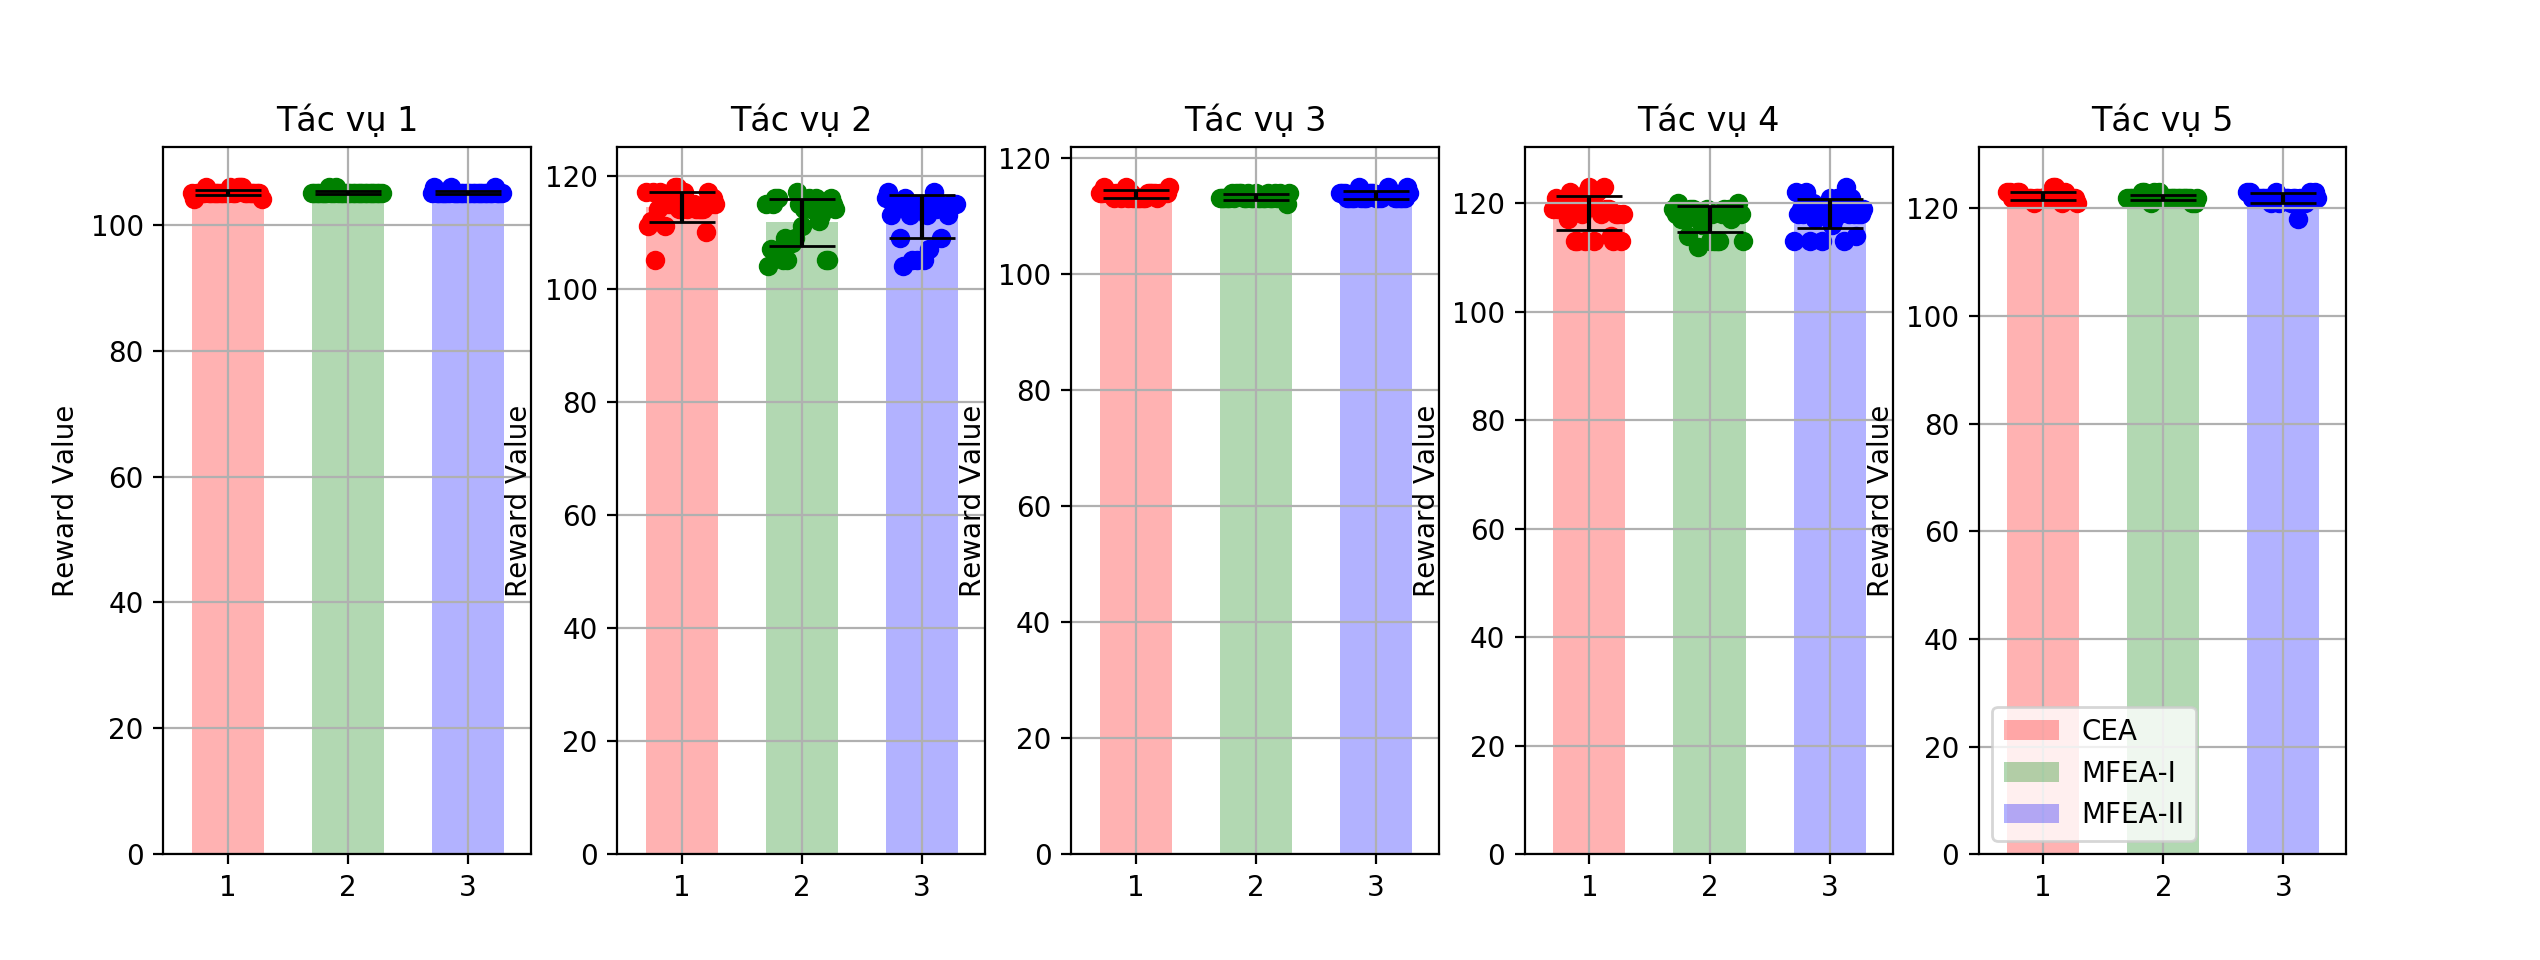
\includegraphics[width=\textwidth,height=\textheight,keepaspectratio]{thesis/images/results/rl/acrobot_final.png}
    \caption{Biểu đồ so sánh mức độ tập trung kết quả cuối cùng cho bài toán Acrobot (khi so sánh trị tuyệt đối của kết quả)}
    \label{fig:Acrobot}
\end{figure}


\subsubsection{Bảng kết quả thực nghiệm - bài toán PixelCopter}
\begin{table} [h!]
    \begin{center}
    \caption{Kết quả huấn luyện các tác vụ cho bài toán PixelCopter}

    \scalebox{0.9}{\begin{tabular}{|c|c|c|c|c|c|}
    \hline
    \multirow{1}{*}{\textbf{Thuật toán}} & \multicolumn{1}{c|}{\textbf{Tác vụ 1}} & \multicolumn{1}{c|}{\textbf{Tác vụ 2}} & \multicolumn{1}{c|}{\textbf{Tác vụ 3}} & \multicolumn{1}{c|}{\textbf{Tác vụ 4}} & \multicolumn{1}{c|}{\textbf{Tác vụ 5}} \\ \hline
    CEA & $101.97 \pm 26.15$ & $104.6 \pm 23.16$ & $96.83 \pm 22.74$ & $96.67 \pm 28.27$ & $93.47 \pm 19.09$ \\
    MFEAI & $124.47 \pm 32.08$ & $125.93 \pm 31.4$ & $123.43 \pm 24.86$ & $122.33 \pm 23.08$ & $120.37 \pm 30.36$  \\
    MFEAII & $\mathbf{133.57 \pm 28.29}$ & $\mathbf{132.03 \pm 33.31}$ & $\mathbf{132.73 \pm 26.93}$ & $\mathbf{129.0 \pm 22.93}$ & $\mathbf{135.4 \pm 30.11}$ \\\hline
    \end{tabular}}
    \end{center}
    \label{tab:result:pixelcopter}
\end{table}


\subsubsection{Biểu đồ hội tụ - bài toán PixelCopter}
\begin{figure}[h!]
    \centering
    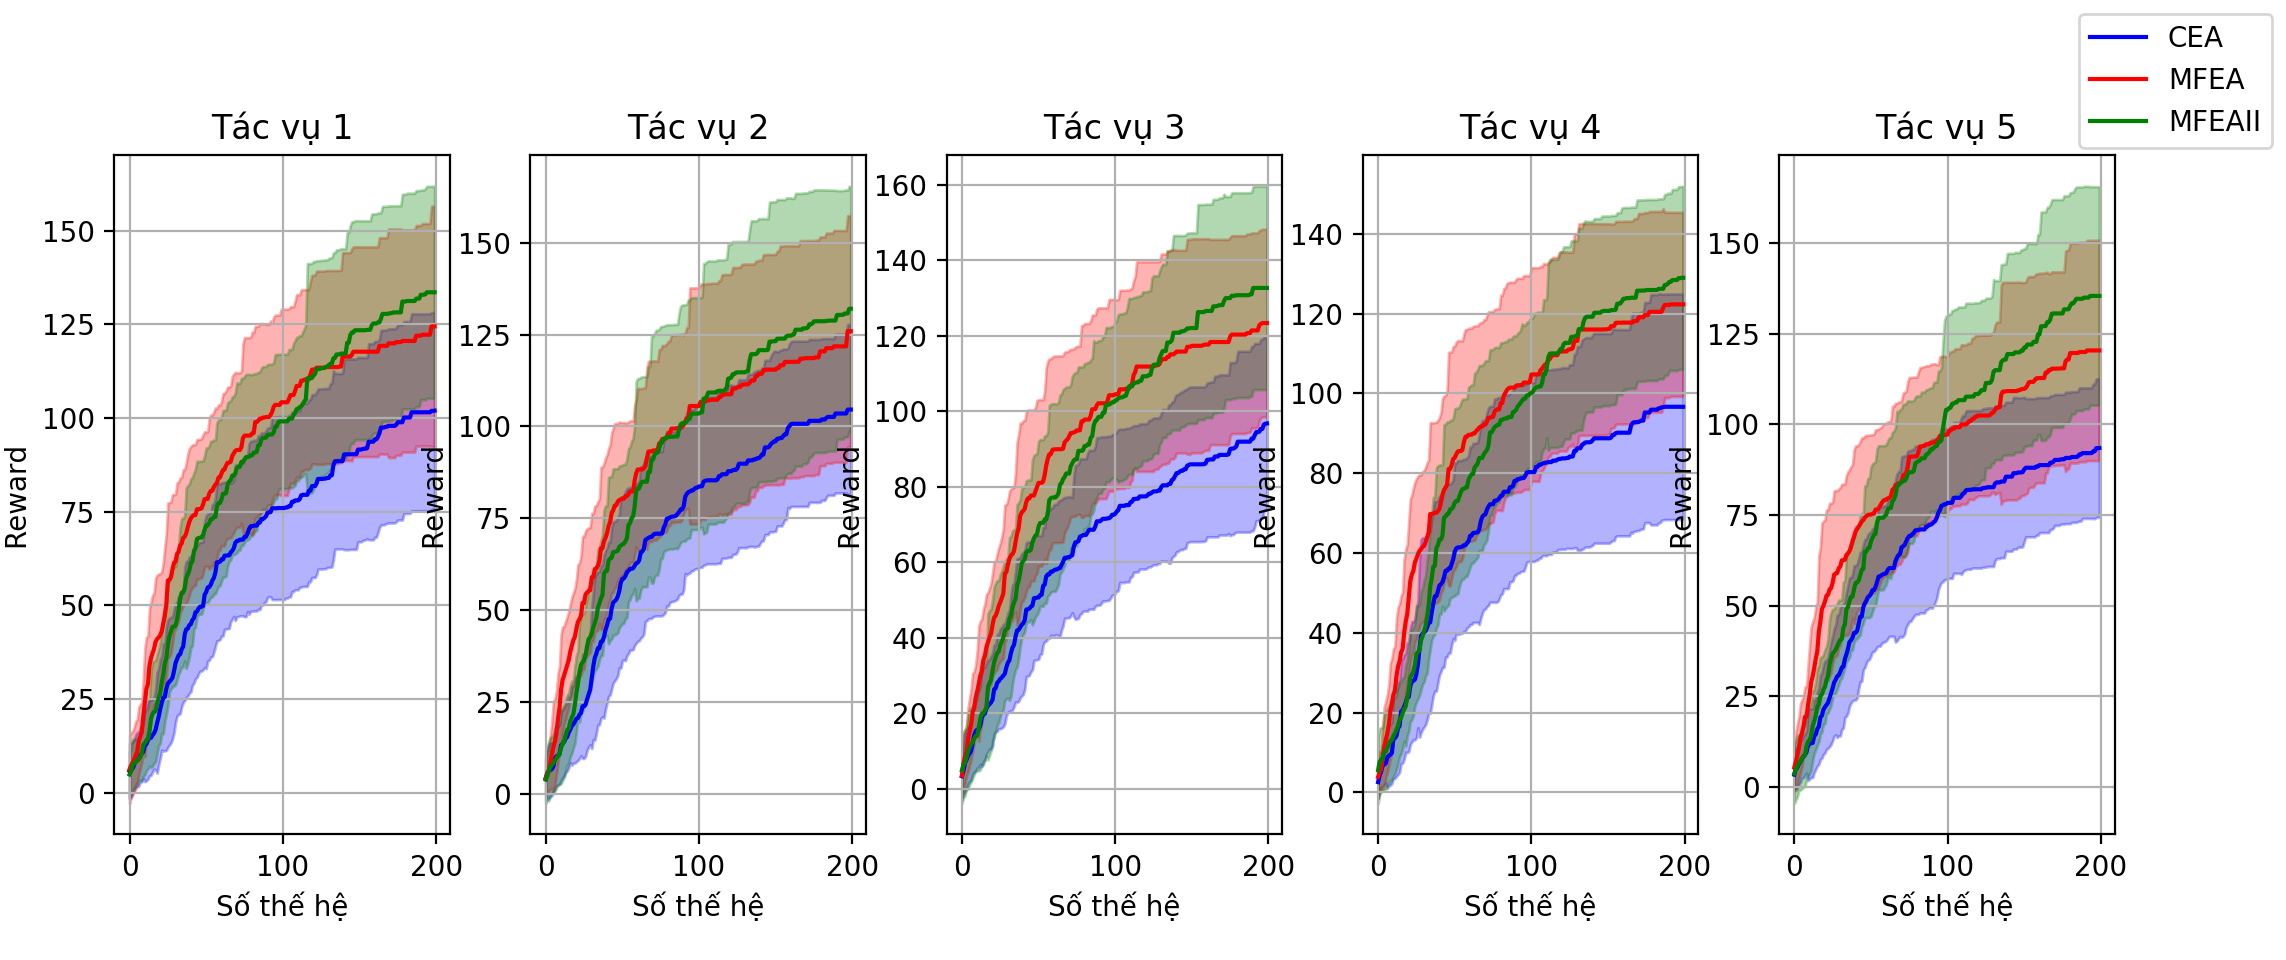
\includegraphics[width=\textwidth,height=\textheight,keepaspectratio]{thesis/images/results/rl/pixcelcopter_conv.png}
    \caption{Biểu đồ hội tụ các tác vụ cho bài toán PixelCopter}
    \label{fig:PixelCopter_conv}
\end{figure}

\subsubsection{So sánh mức độ tập trung kết quả cuối cùng - bài toán PixelCopter}
\begin{figure}[h!]
    \centering
    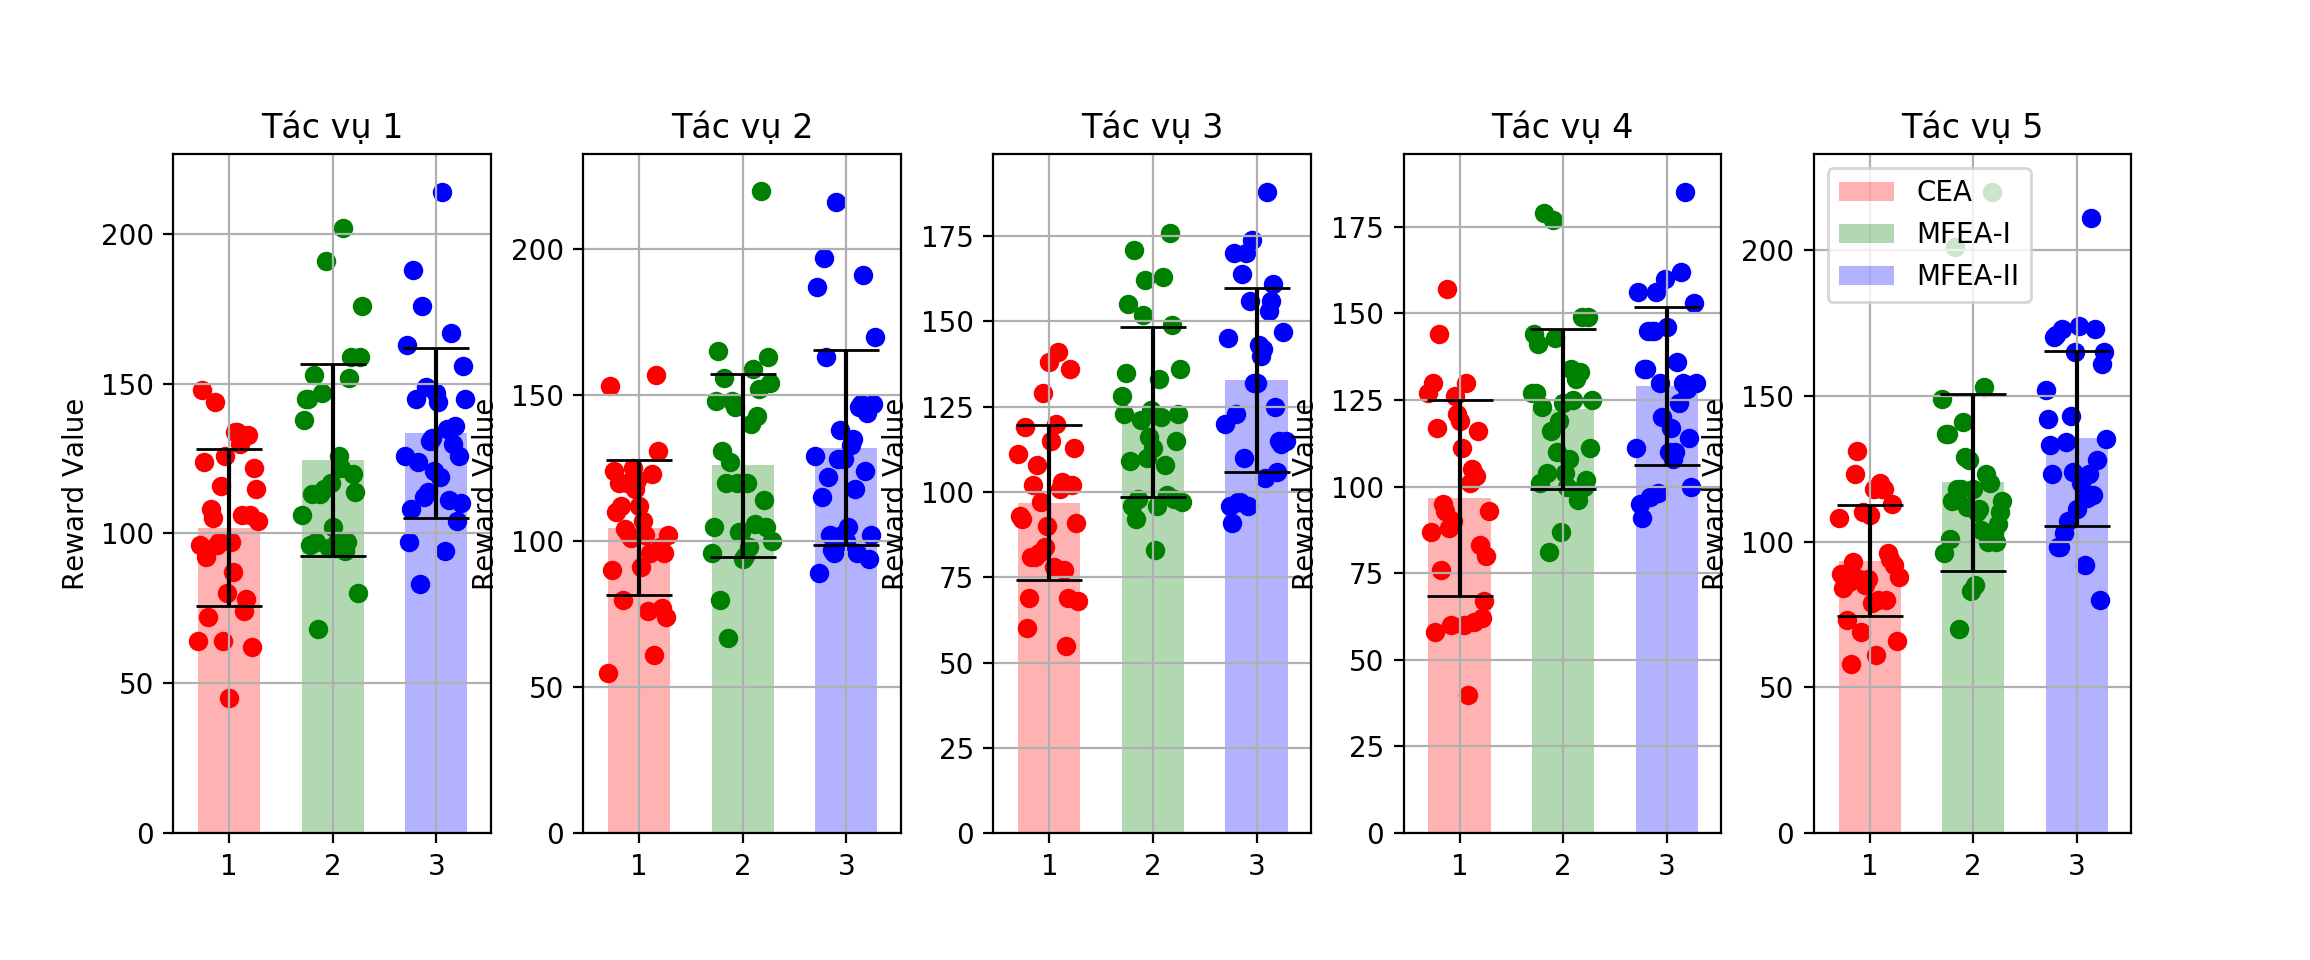
\includegraphics[width=\textwidth,height=\textheight,keepaspectratio]{thesis/images/results/rl/pixelcopter_final.png}
    \caption{Biểu đồ so sánh mức độ tập trung kết quả cuối cùng cho bài toán PixelCopter}
    \label{fig:PixelCopter}
\end{figure}
\subsubsection{Bảng kết quả thực nghiệm - bài toán FlappyBird}
\begin{table} [H]
    \begin{center}
    \caption{Kết quả huấn luyện các tác vụ cho bài toán FlappyBird}

    \scalebox{0.9}{\begin{tabular}{|c|c|c|c|c|c|}
    \hline
    \multirow{1}{*}{\textbf{Thuật toán}} & \multicolumn{1}{c|}{\textbf{Tác vụ 1}} & \multicolumn{1}{c|}{\textbf{Tác vụ 2}} & \multicolumn{1}{c|}{\textbf{Tác vụ 3}} & \multicolumn{1}{c|}{\textbf{Tác vụ 4}} & \multicolumn{1}{c|}{\textbf{Tác vụ 5}} \\ \hline
    CEA & $25.9 \pm 17.57$ & $219.1 \pm 151.39$ & $101.8 \pm 88.65$ & $78.77 \pm 62.43$ & $24.63 \pm 23.62$ \\
    MFEAI & $47.43 \pm 17.97$ & $\mathbf{319.83 \pm 118.9}$ & $\mathbf{217.87 \pm 48.57}$ & $142.9 \pm 26.86$ & $90.17 \pm 20.69$ \\
    MFEAII & $\mathbf{50.93 \pm 16.47}$ & $314.07 \pm 116.25$ & $214.83 \pm 51.96$ & $\mathbf{145.47 \pm 26.72}$ & $\mathbf{105.33 \pm 26.12}$ \\\hline
    \end{tabular}}
    \end{center}
    \label{tab:result:pixelcopter}
\end{table}


\subsubsection{Biểu đồ hội tụ - bài toán FlappyBird}
\begin{figure}[h!]
    \centering
    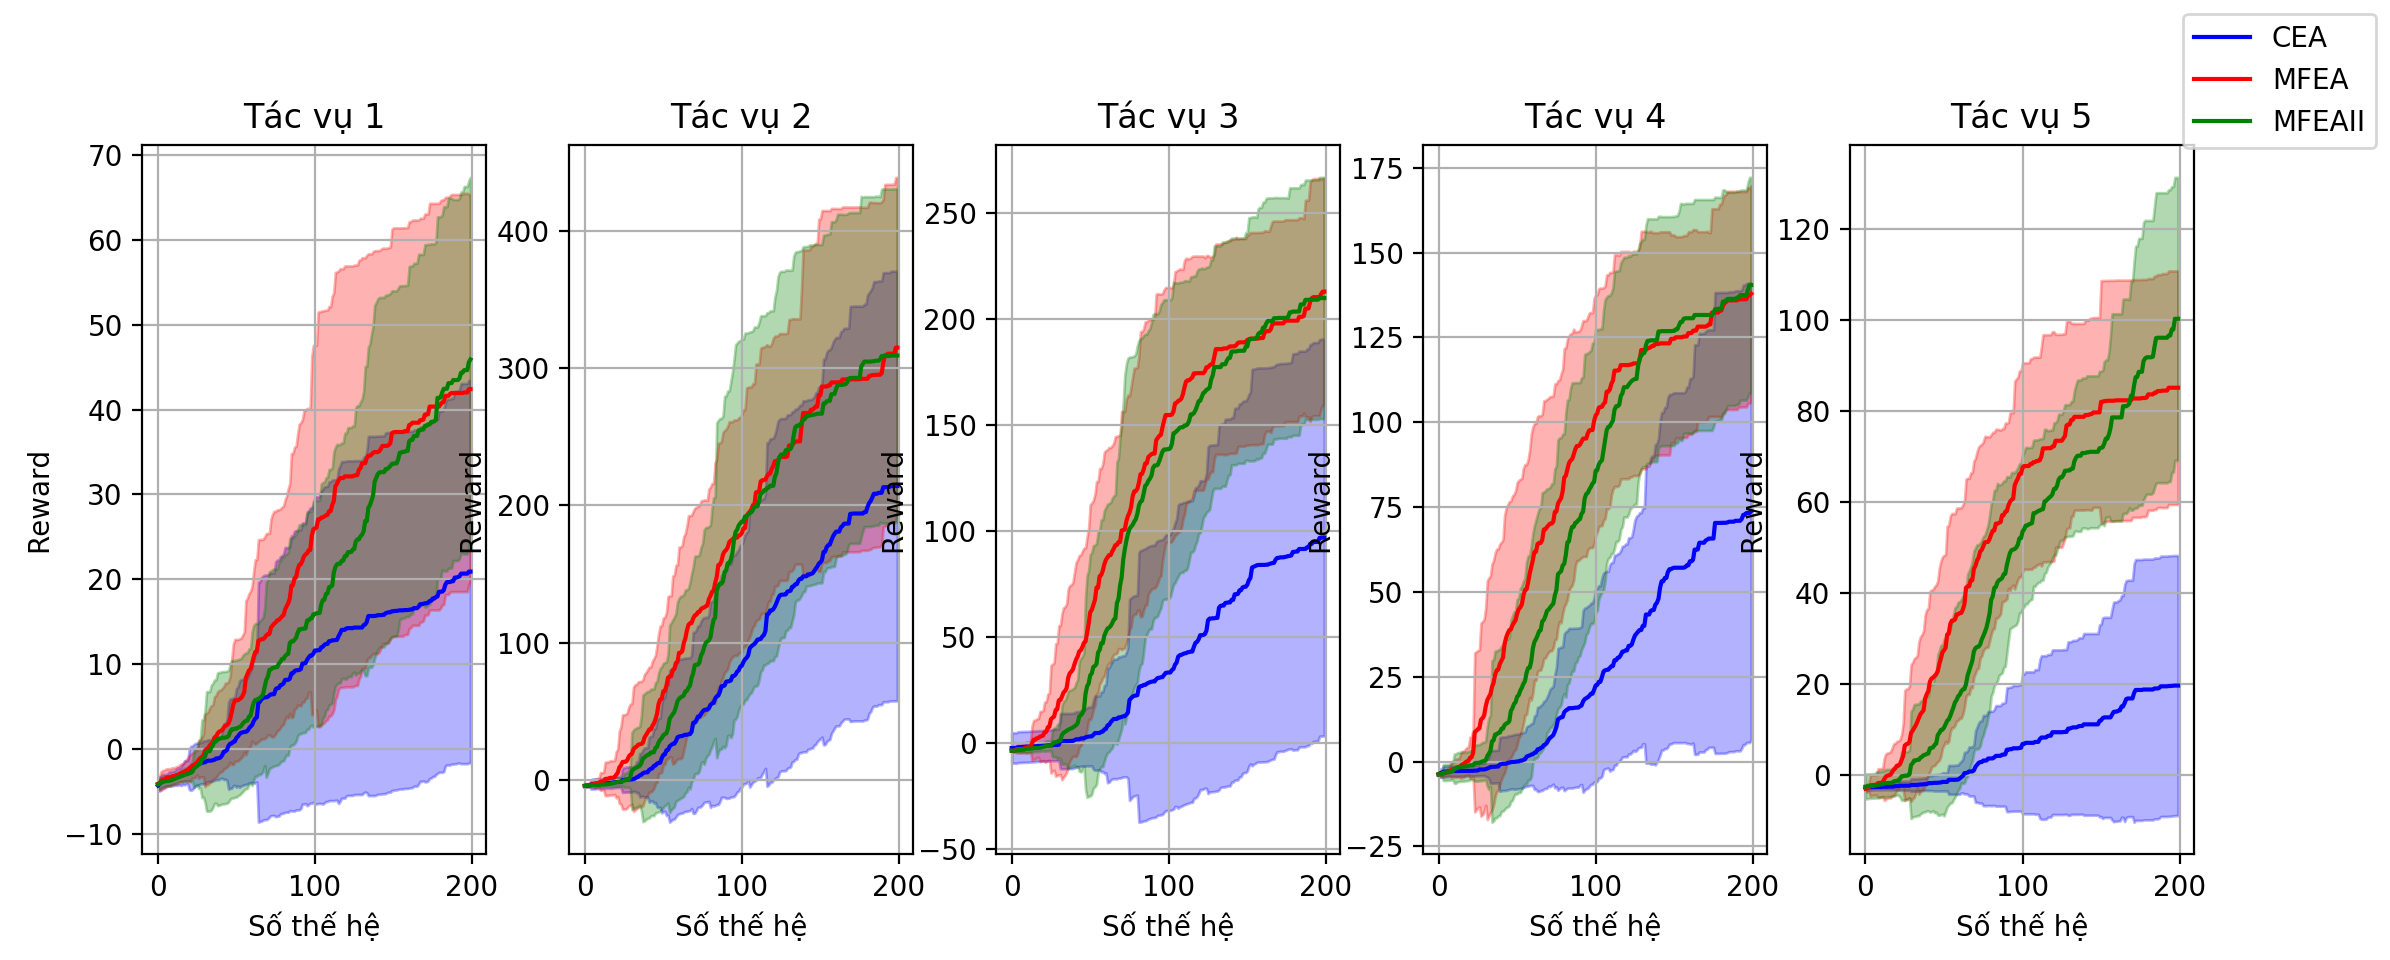
\includegraphics[width=\textwidth,height=\textheight,keepaspectratio]{thesis/images/results/rl/flappybird_conv.png}
    \caption{Biểu đồ hội tụ các tác vụ cho bài toán FlappyBird}
    \label{fig:FLP_conv}
\end{figure}

\subsubsection{So sánh mức độ tập trung kết quả cuối cùng - bài toán FlappyBird}
\begin{figure}[h!]
    \centering
    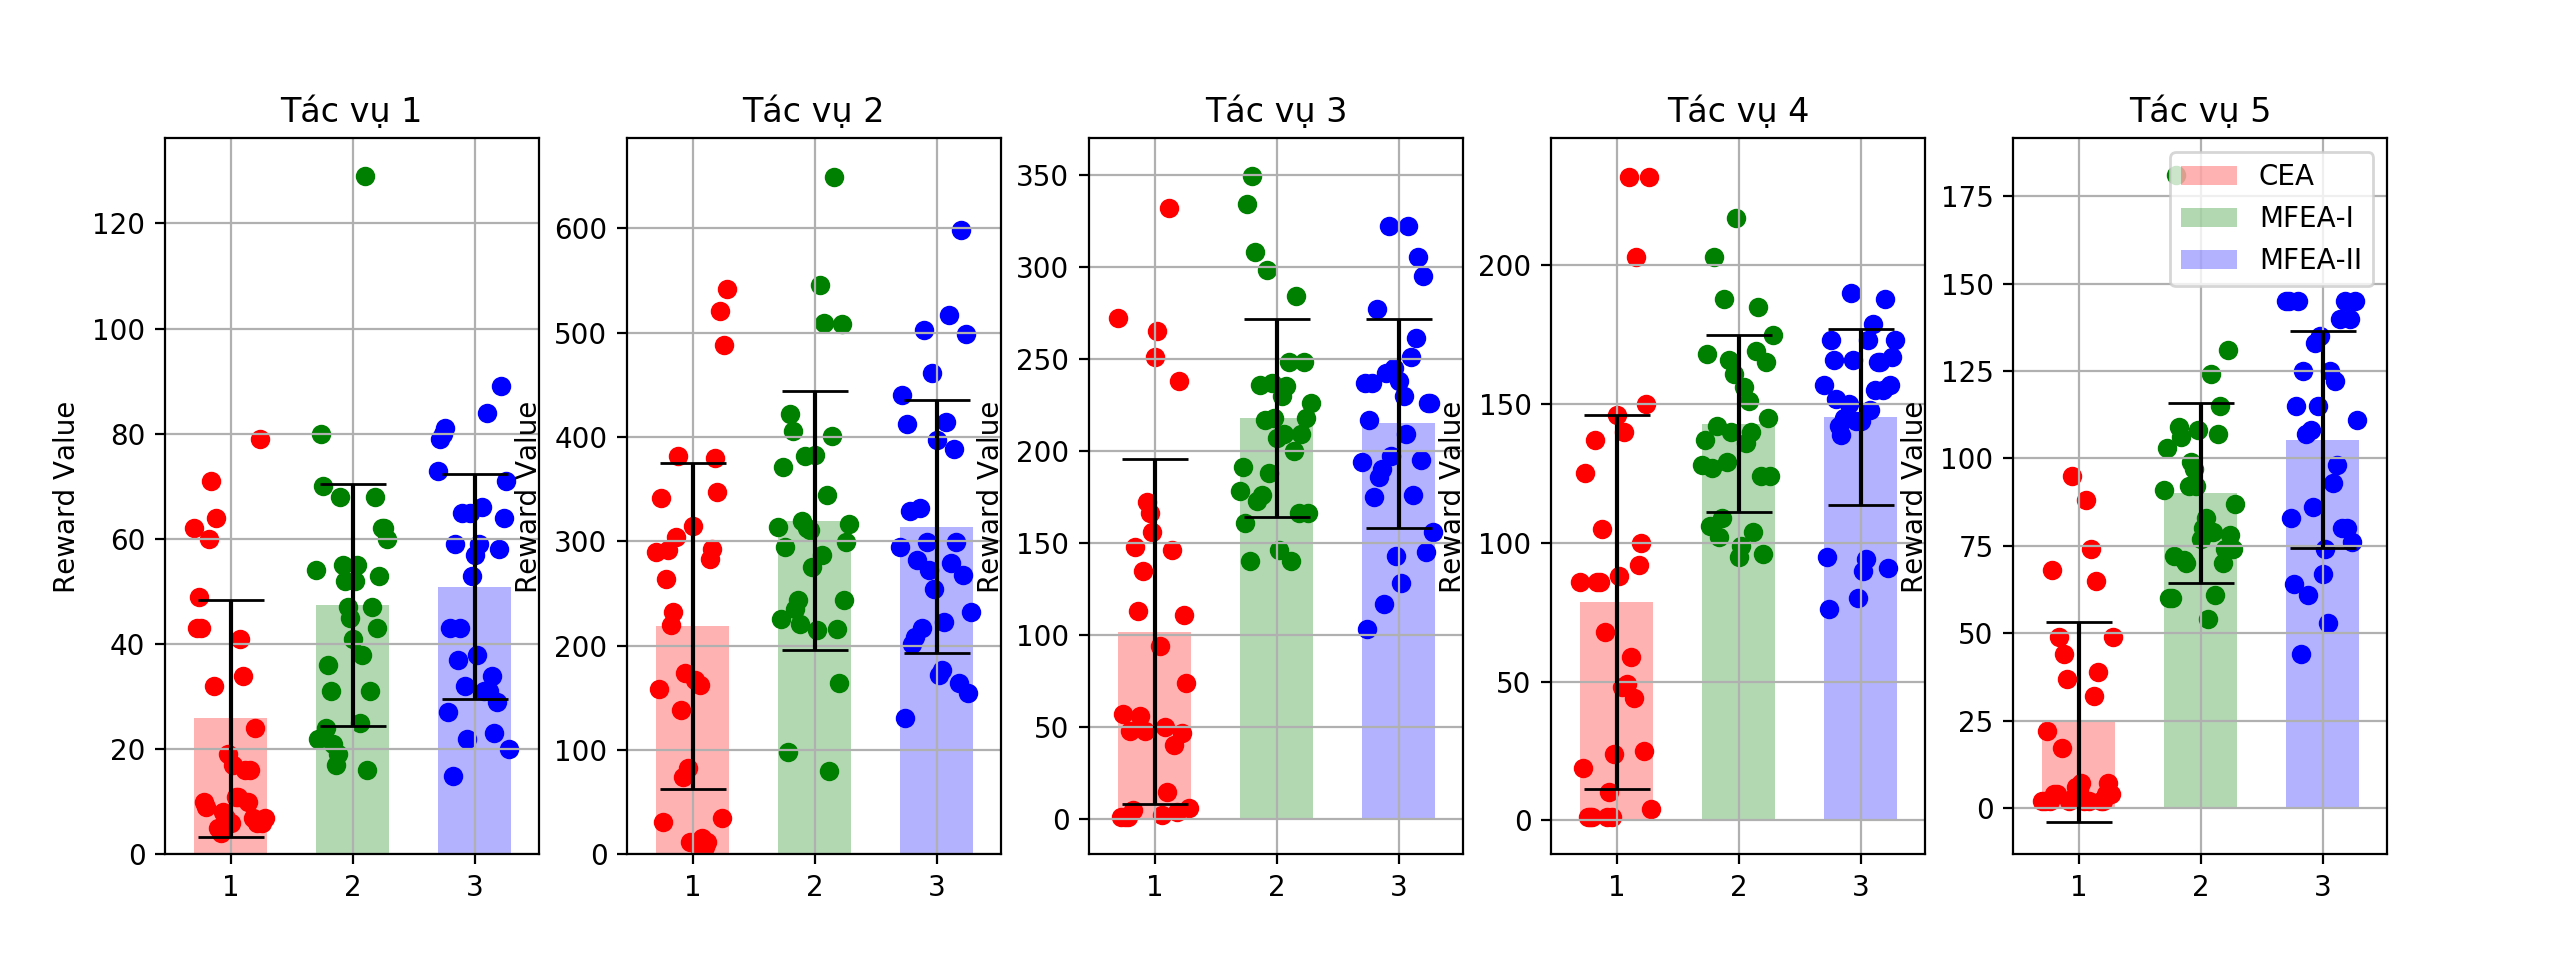
\includegraphics[width=\textwidth,height=\textheight,keepaspectratio]{thesis/images/results/rl/flappybird_final.png}
    \caption{Biểu đồ so sánh mức độ tập trung kết quả cuối cùng cho bài toán FlappyBird}
    \label{fig:FLP}
\end{figure}
